\chapter{}
\section{L1 Jet Energy Correction Fits}
\label{app:jecfits}
The energy corrections applied online at L1 to jets are derived in 11 $|\eta|$ bins
corresponding to the 11 regions of the GCT. The values of the fitted parameters
in each bin for the parameterisation in Equation~\ref{eqn:jecfit} are 
given in Table~\ref{tab:calibrationcoeffs}. These parameter values are extracted from 
fitting the L1 response as a function of $\Lonept$ as described in 
Section~\ref{sec:jetenergyresponse}. Figures~\ref{fig:allcorrfuncsp1} 
and~\ref{fig:allcorrfuncsp2} show the results of those fits in each $|\eta|$ bin.

\begin{table}
\centering
\begin{tabular}{| c | c | c | c | c | c | c |}
\hline
 & $p_{0}$ & $p_{1}$ & $p_{2}$ & $p_{3}$ & $p_{4}$ & $p_{5}$ \\
\hline
$0<|\eta|<0.348$            &1.114      &2.297  &5.959  &1.181  &0.7286 &0.3673         \\
$0.348<|\eta|<0.695$    &0.7842 &4.331  &2.672  &0.5743 &0.8811 &0.4085         \\
$0.695<|\eta|<1.044$    &0.961  &2.941  &2.4      &1.248        &0.666  &0.1041         \\
$1.044<|\eta|<1.392$    &0.6318 &6.6      &3.21         &0.8551 &0.9786 &0.291          \\
$1.392<|\eta|<1.740$    &0.3456 &8.992  &3.165  &0.5798 &2.146  &0.4912         \\
$1.740<|\eta|<2.172$    &0.8501 &3.892  &2.466  &1.236  &0.8323 &0.1809         \\
$2.172<|\eta|<3.0$        &0.9027       &2.581  &1.453  &1.029  &0.6767 &-0.1476        \\
$3.0<|\eta|<3.5$      &1.117    &2.382  &1.769  &0.0      &-1.306 &-0.4741      \\
$3.5<|\eta|<4.0$      &1.634    &-1.01  &0.7184 &1.639  &0.6727 &-0.2129        \\
$4.0<|\eta|<4.5$      &0.9862 &3.138    &4.672  &2.362  &1.55   &-0.7154        \\
$4.5<|\eta|<5.0$      &1.245    &1.103  &1.919  &0.3054 &5.745  &0.8622 \\ 
\hline
\end{tabular}   
\caption{Calibration coefficients used to parameterise the L1 jet correction function
 (Equation~\ref{eqn:jecfit}) for each of the 11 GCT regions.}
\label{tab:calibrationcoeffs}
\end{table}

\begin{figure}
\begin{center}
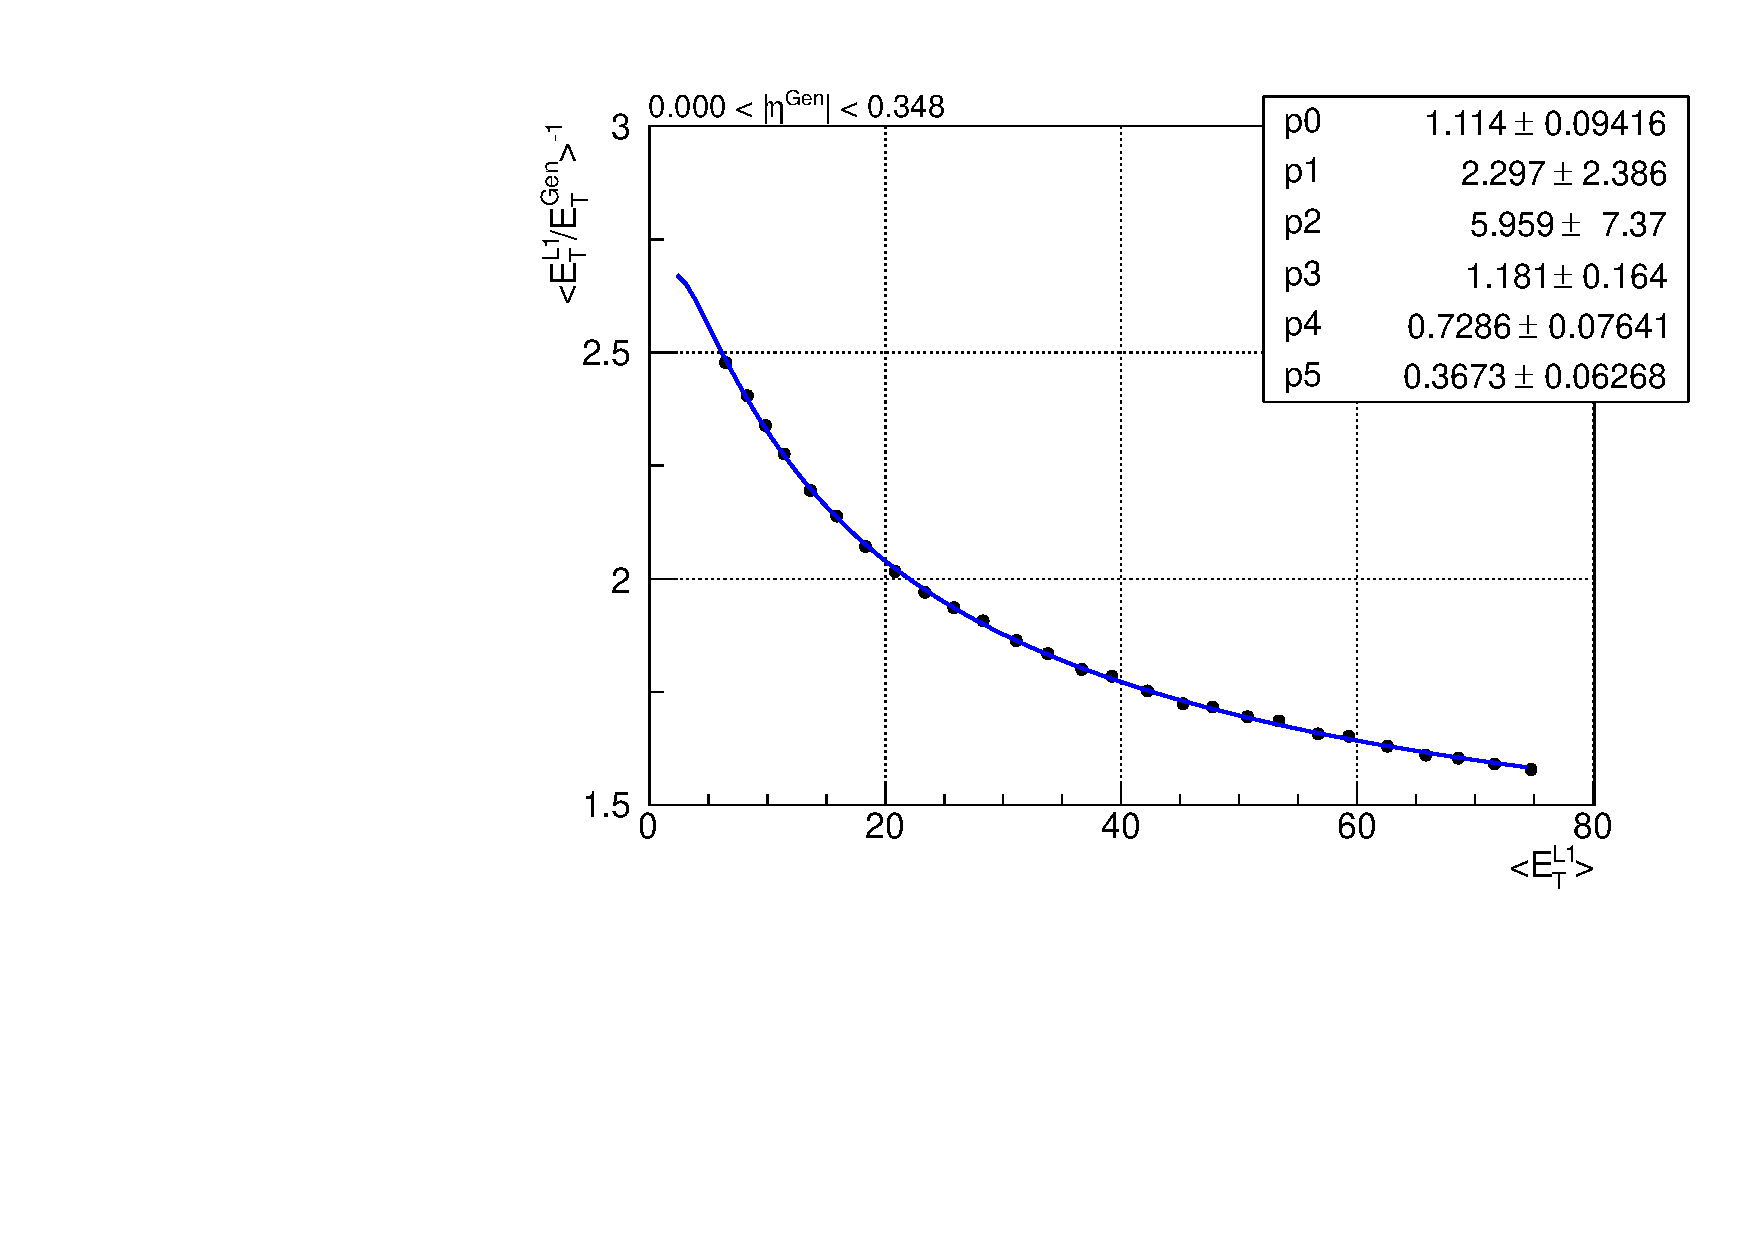
\includegraphics[width=0.49\textwidth]{detector/l1jet/egcor0.pdf}
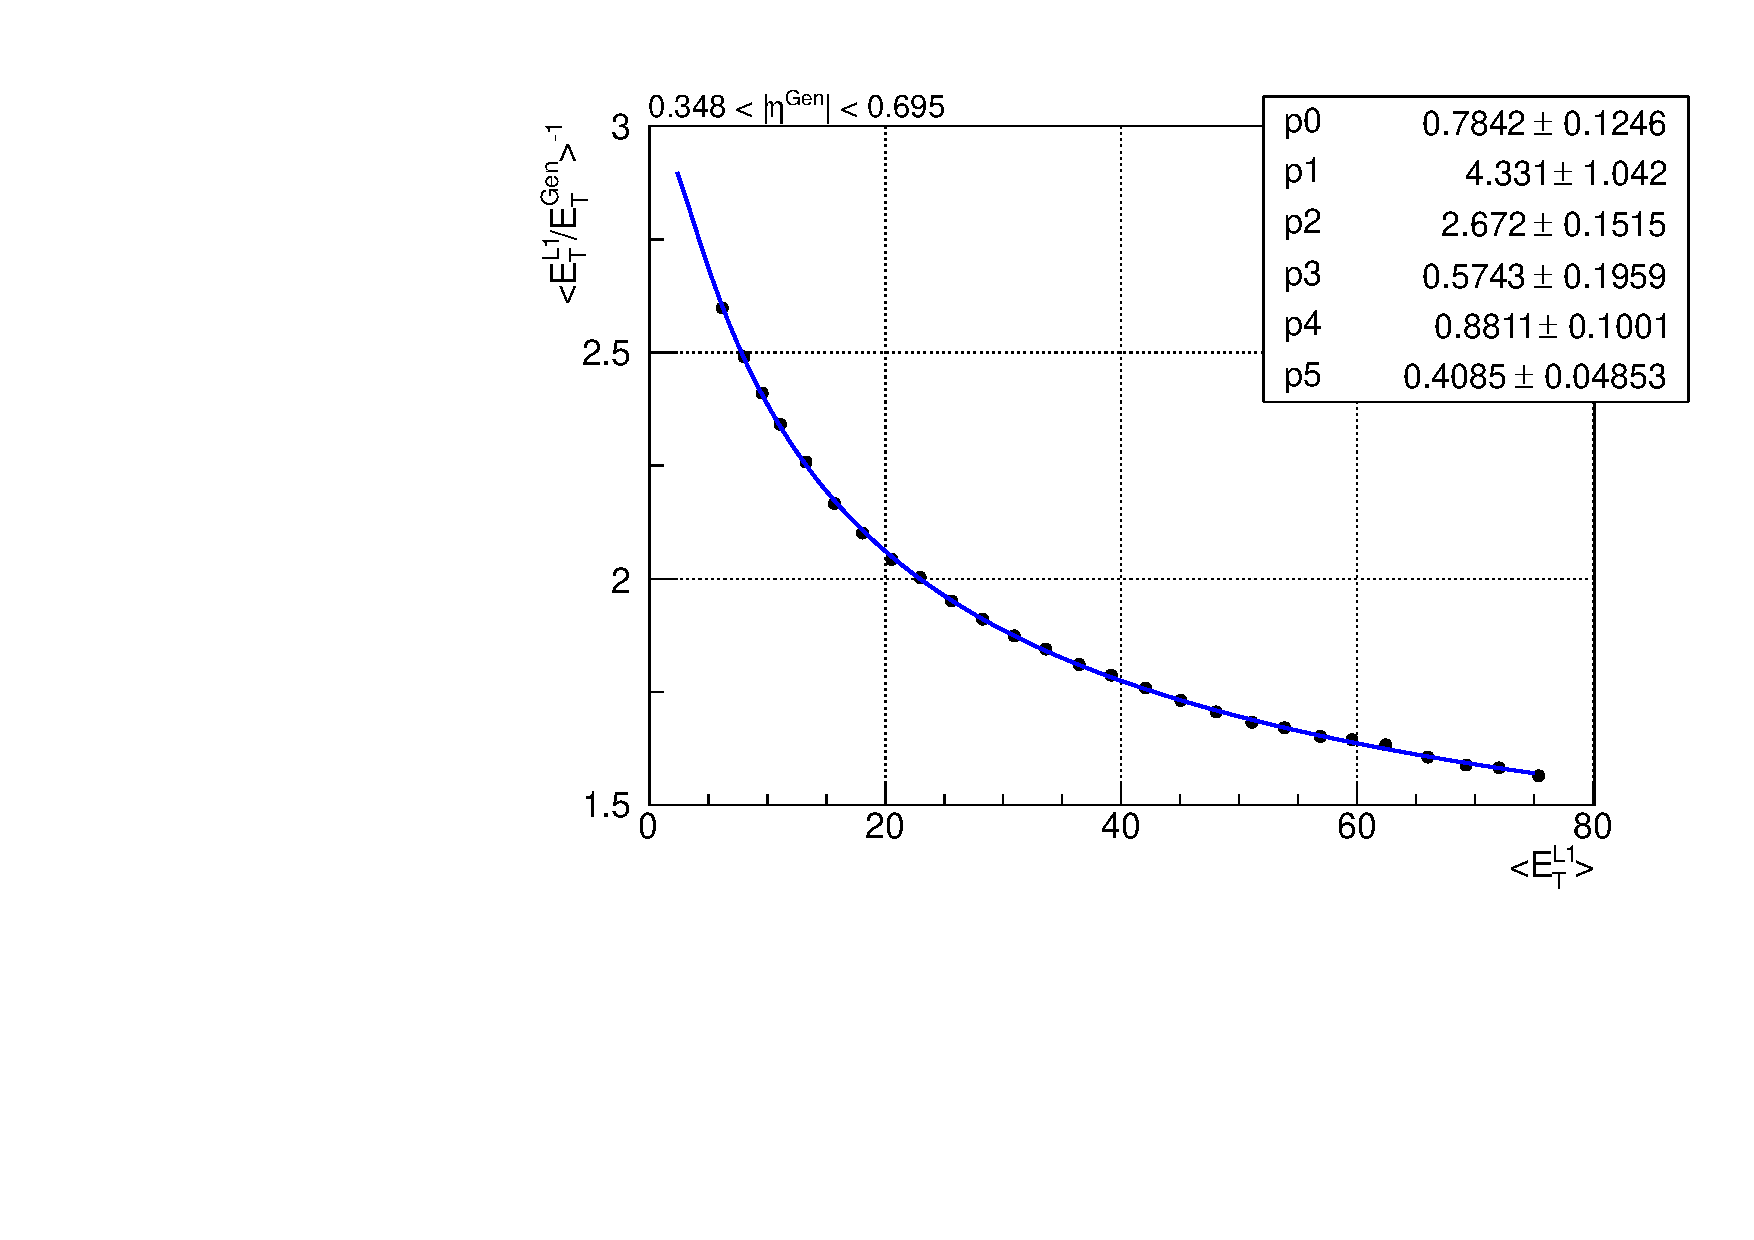
\includegraphics[width=0.49\textwidth]{detector/l1jet/egcor1.pdf}\\
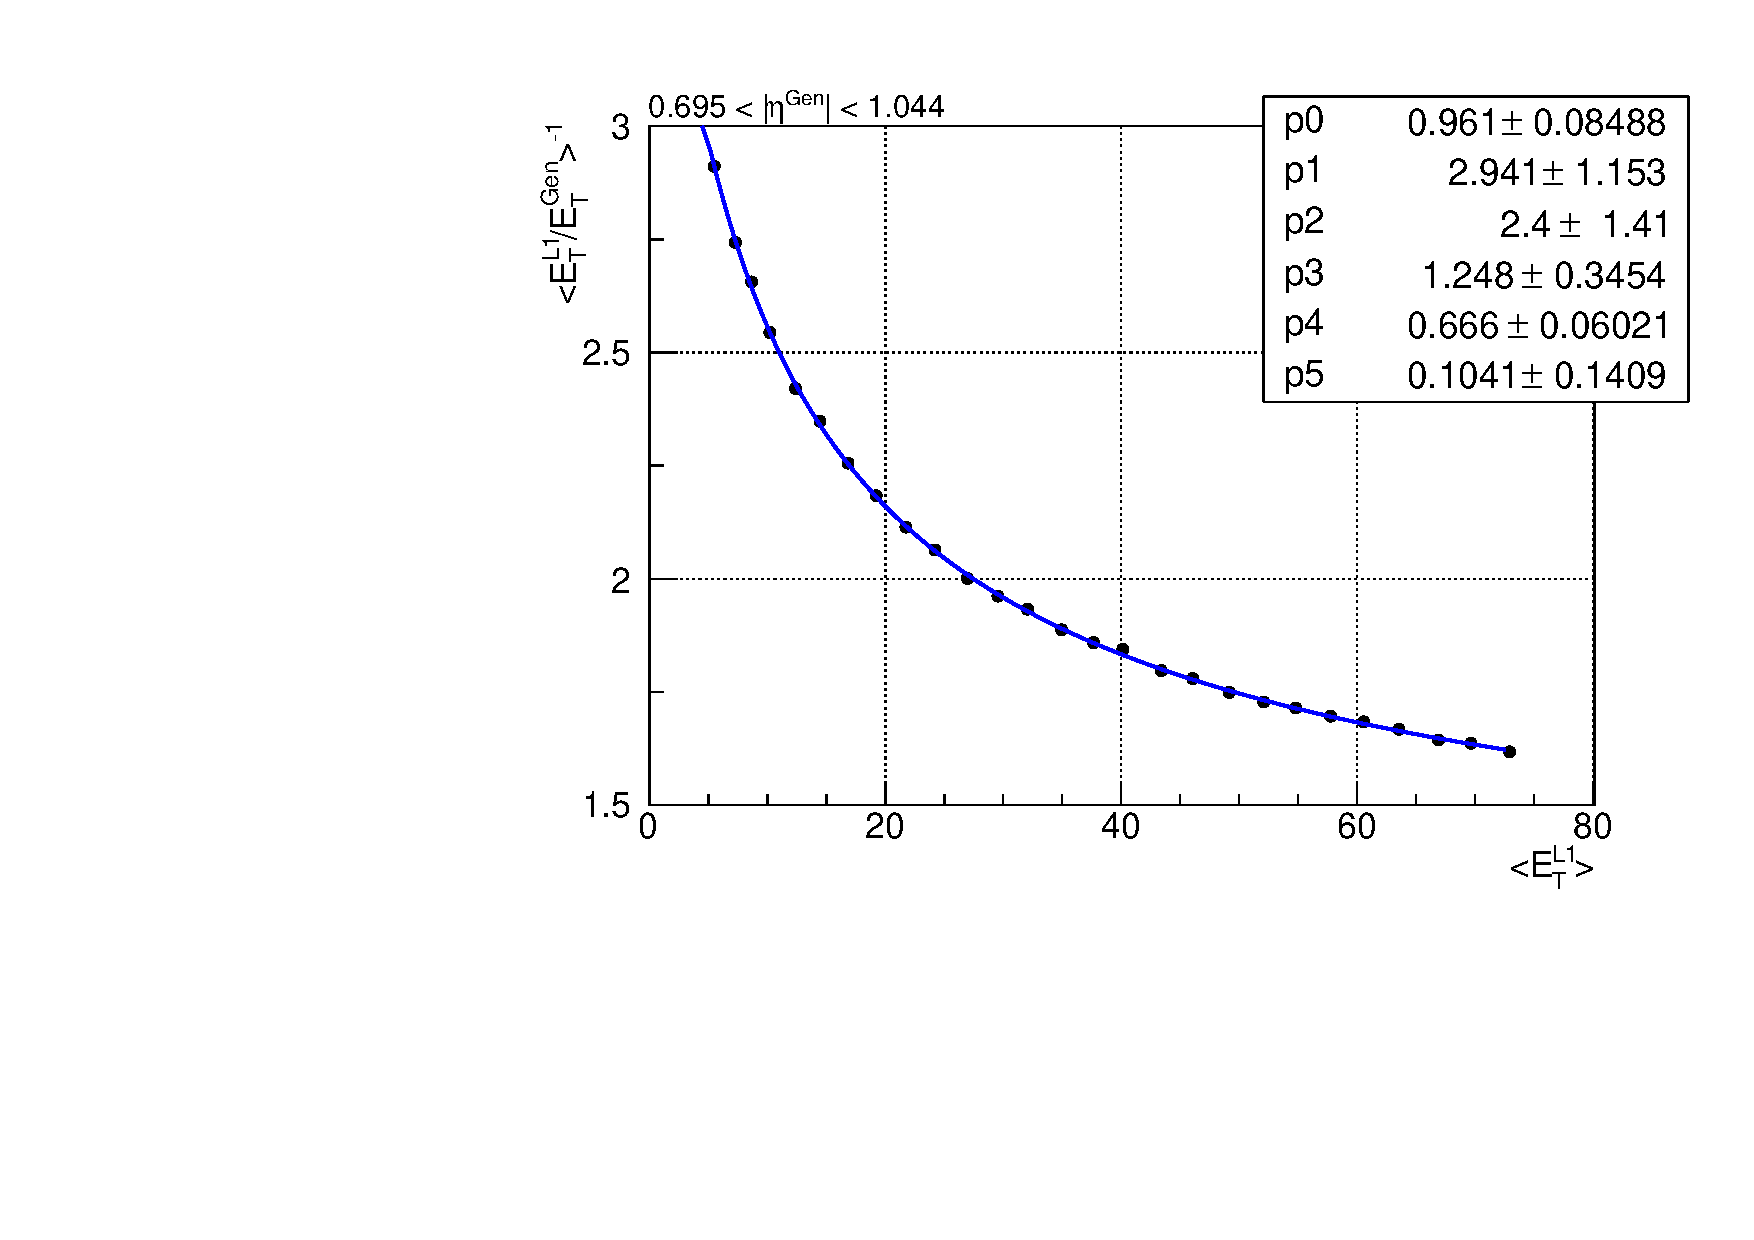
\includegraphics[width=0.49\textwidth]{detector/l1jet/egcor2.pdf}
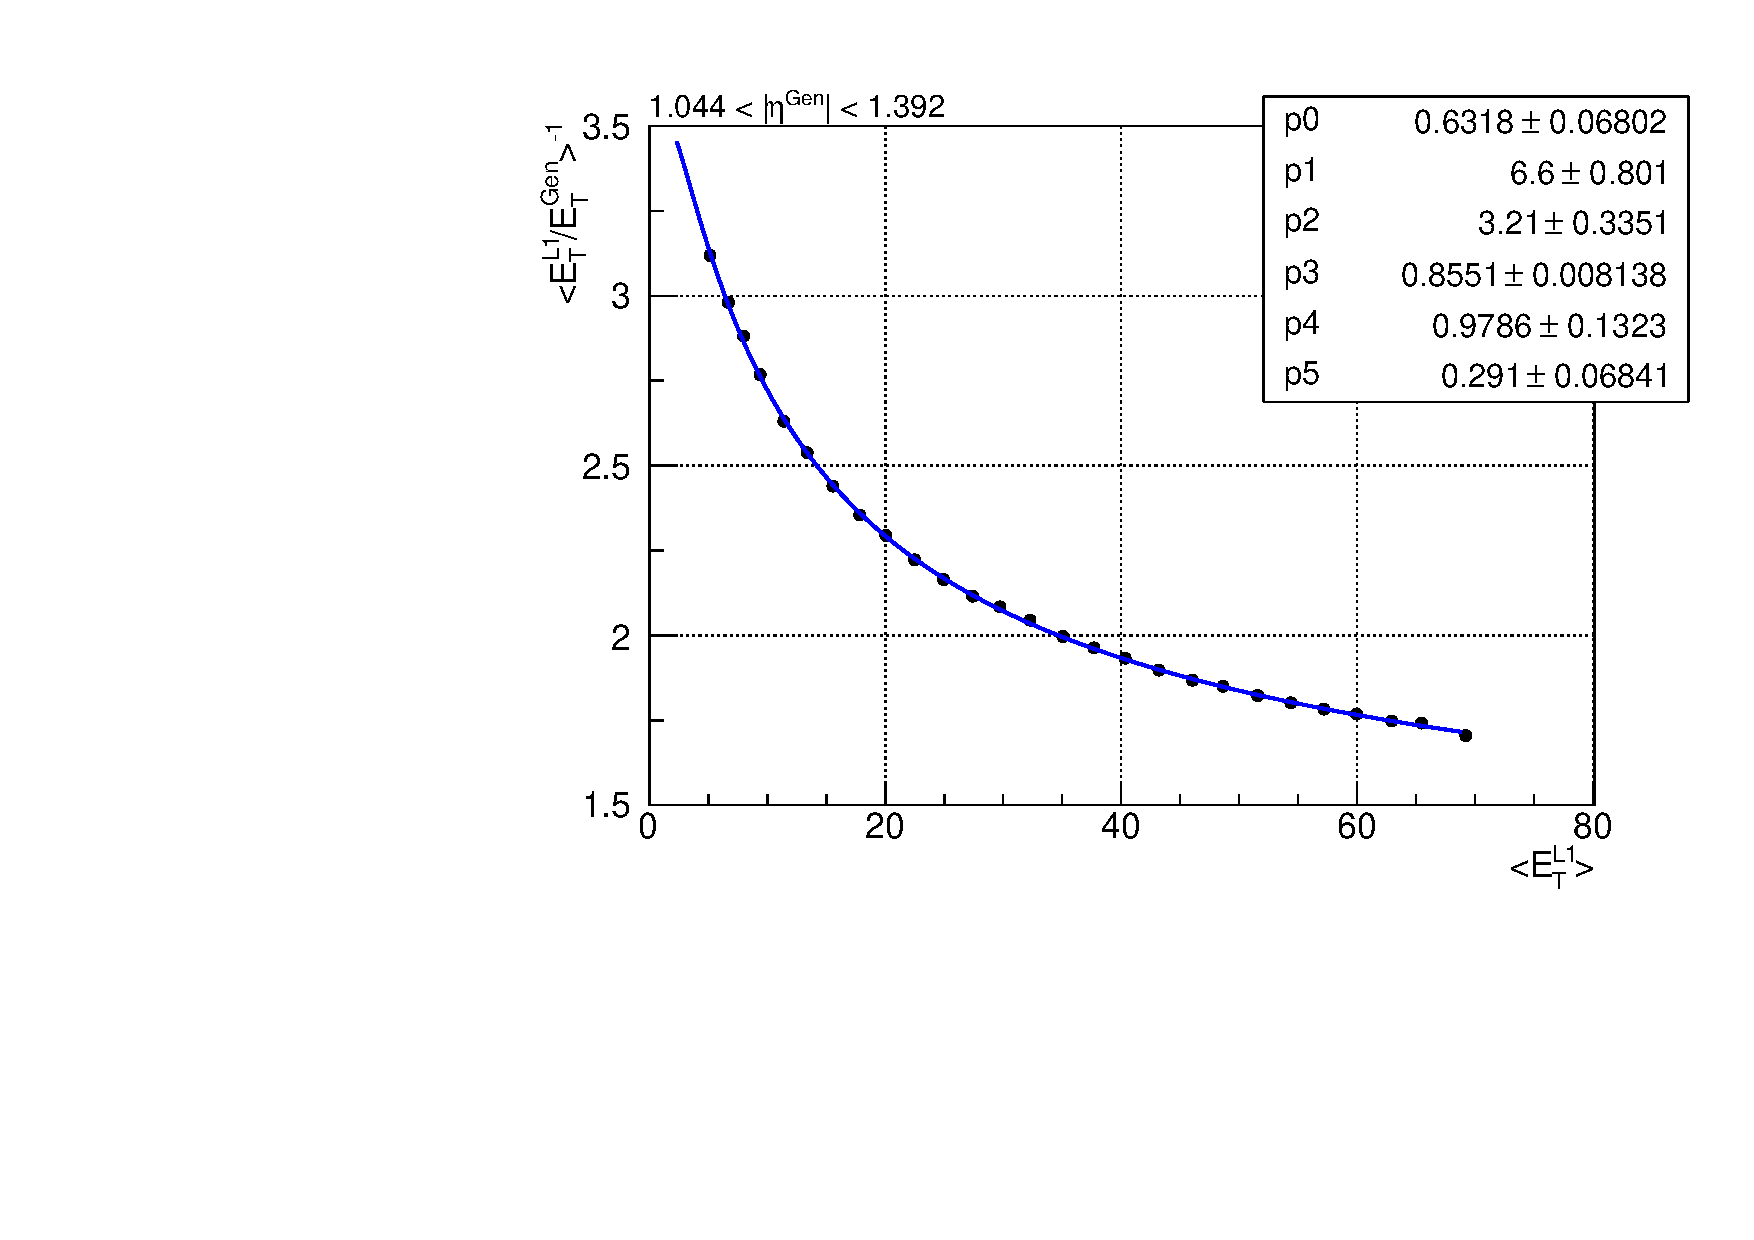
\includegraphics[width=0.49\textwidth]{detector/l1jet/egcor3.pdf}\\
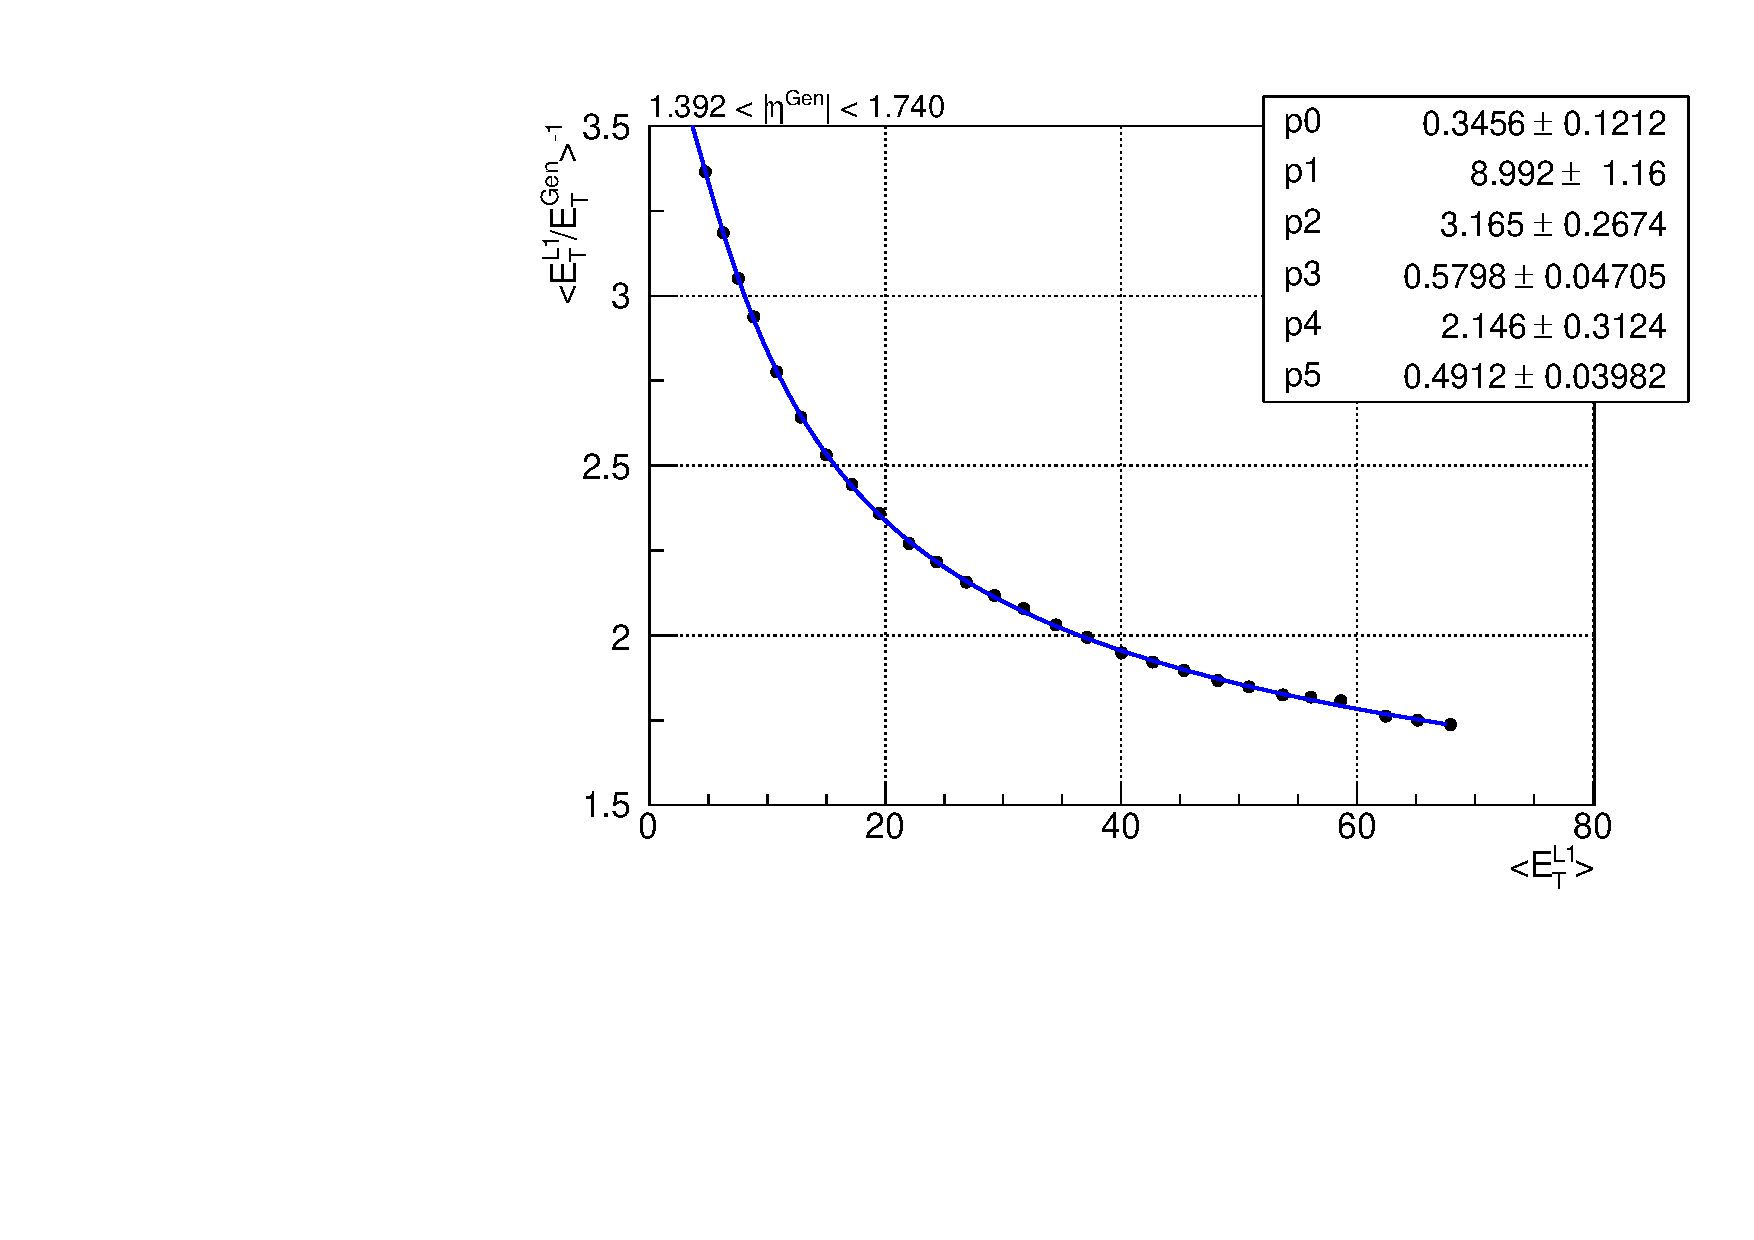
\includegraphics[width=0.49\textwidth]{detector/l1jet/egcor4.pdf}
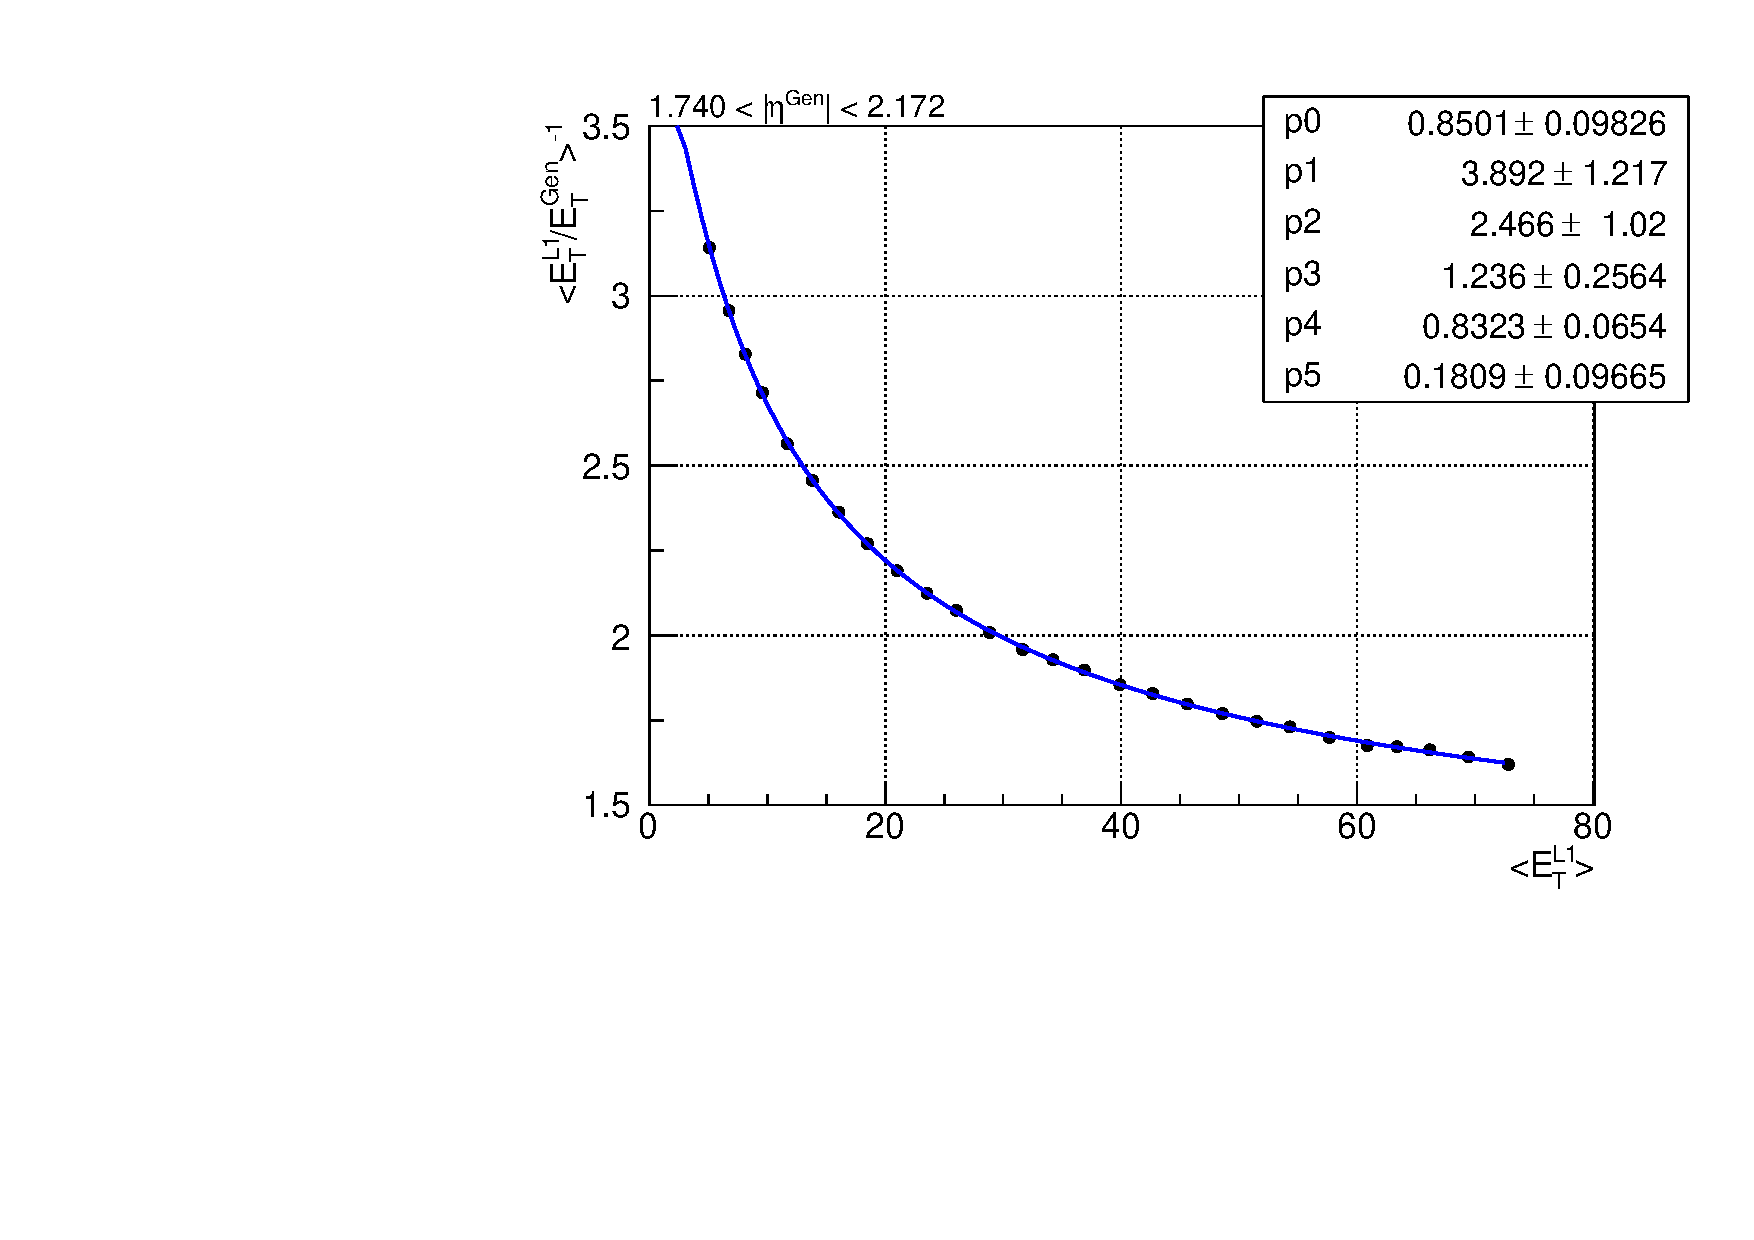
\includegraphics[width=0.49\textwidth]{detector/l1jet/egcor5.pdf}\\
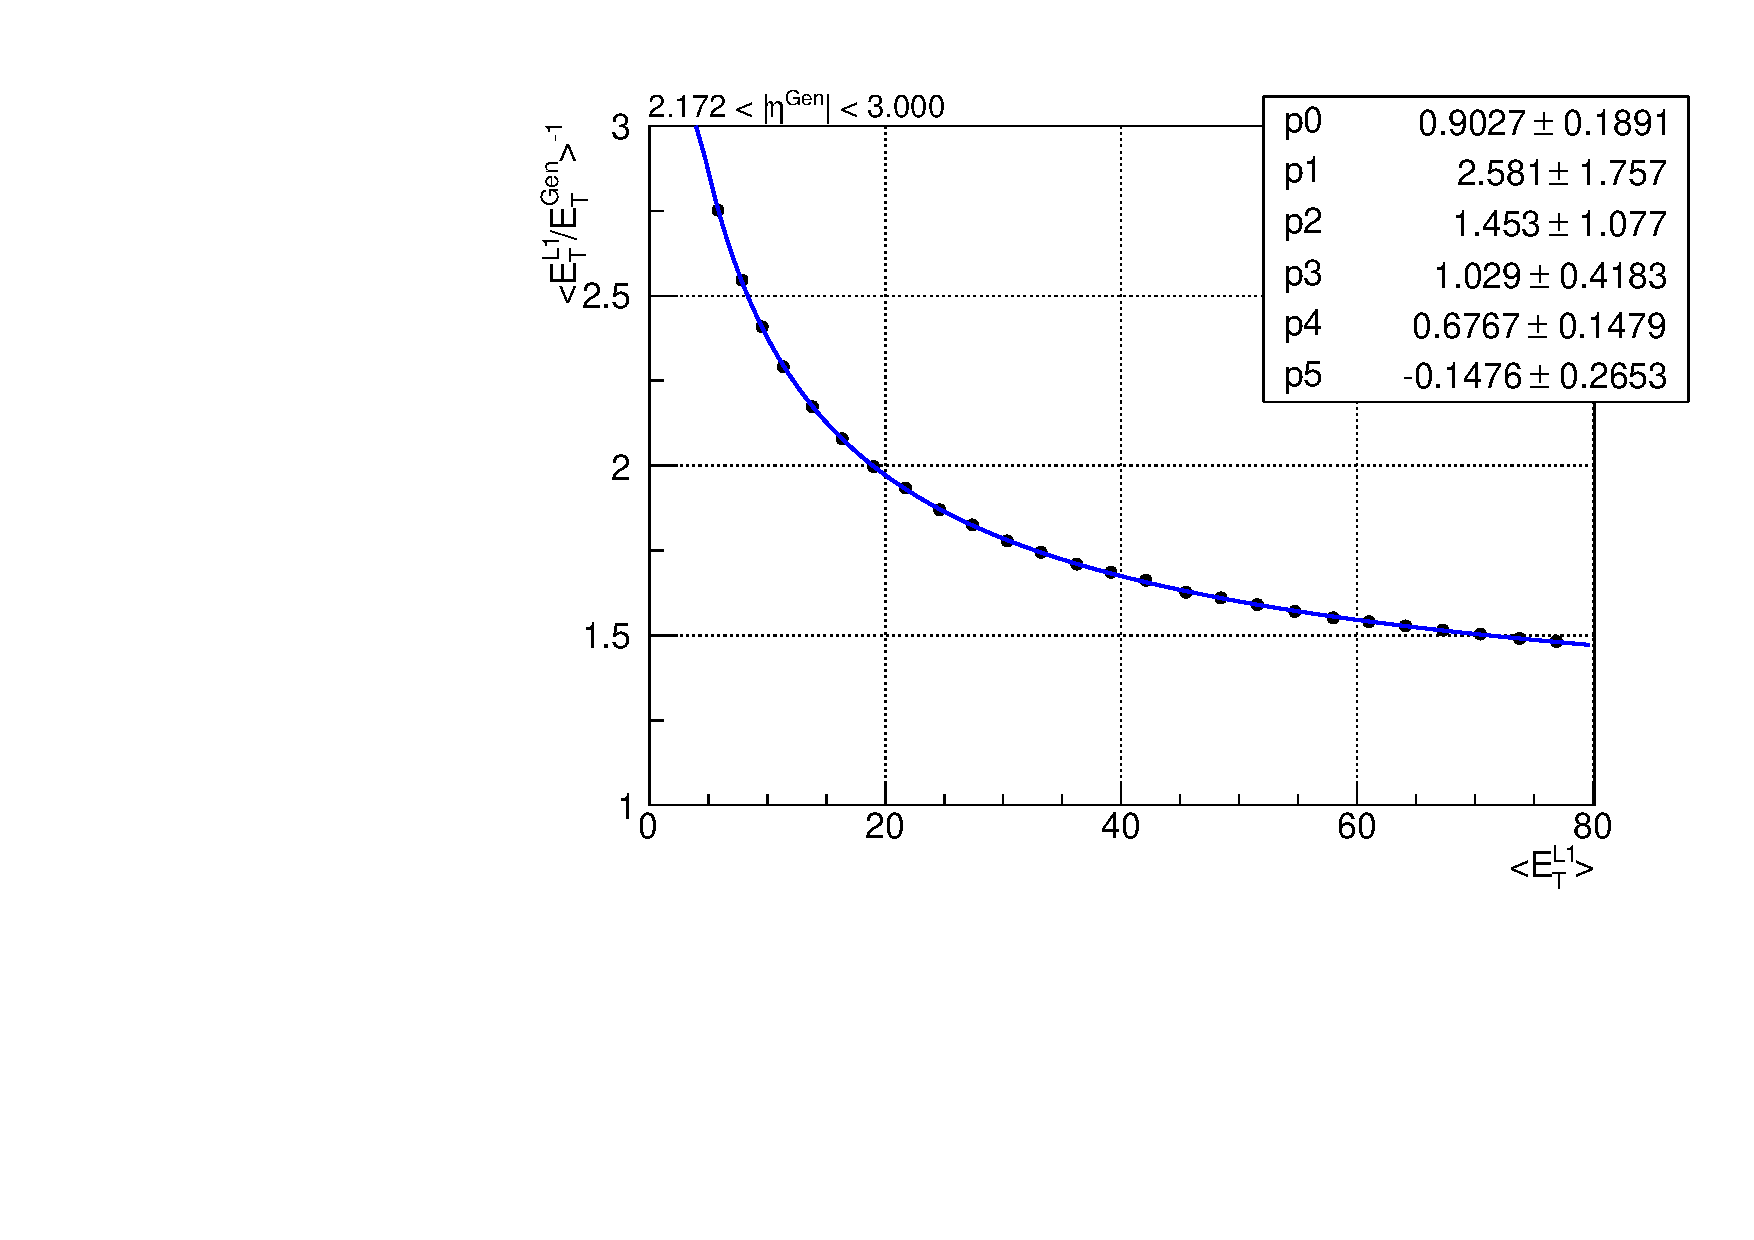
\includegraphics[width=0.49\textwidth]{detector/l1jet/egcor6.pdf}
\end{center}
\caption{Fitted correction functions for each of the 7 GCT regions covered
by the ECAL and HCAL. 
The points are fit with the function of Equation~\ref{eqn:jecfit}  to 
provide a parameterisation of the corrections to be applied to L1 jets.}
\label{fig:allcorrfuncsp1}
\end{figure}

\begin{figure}
\begin{center}
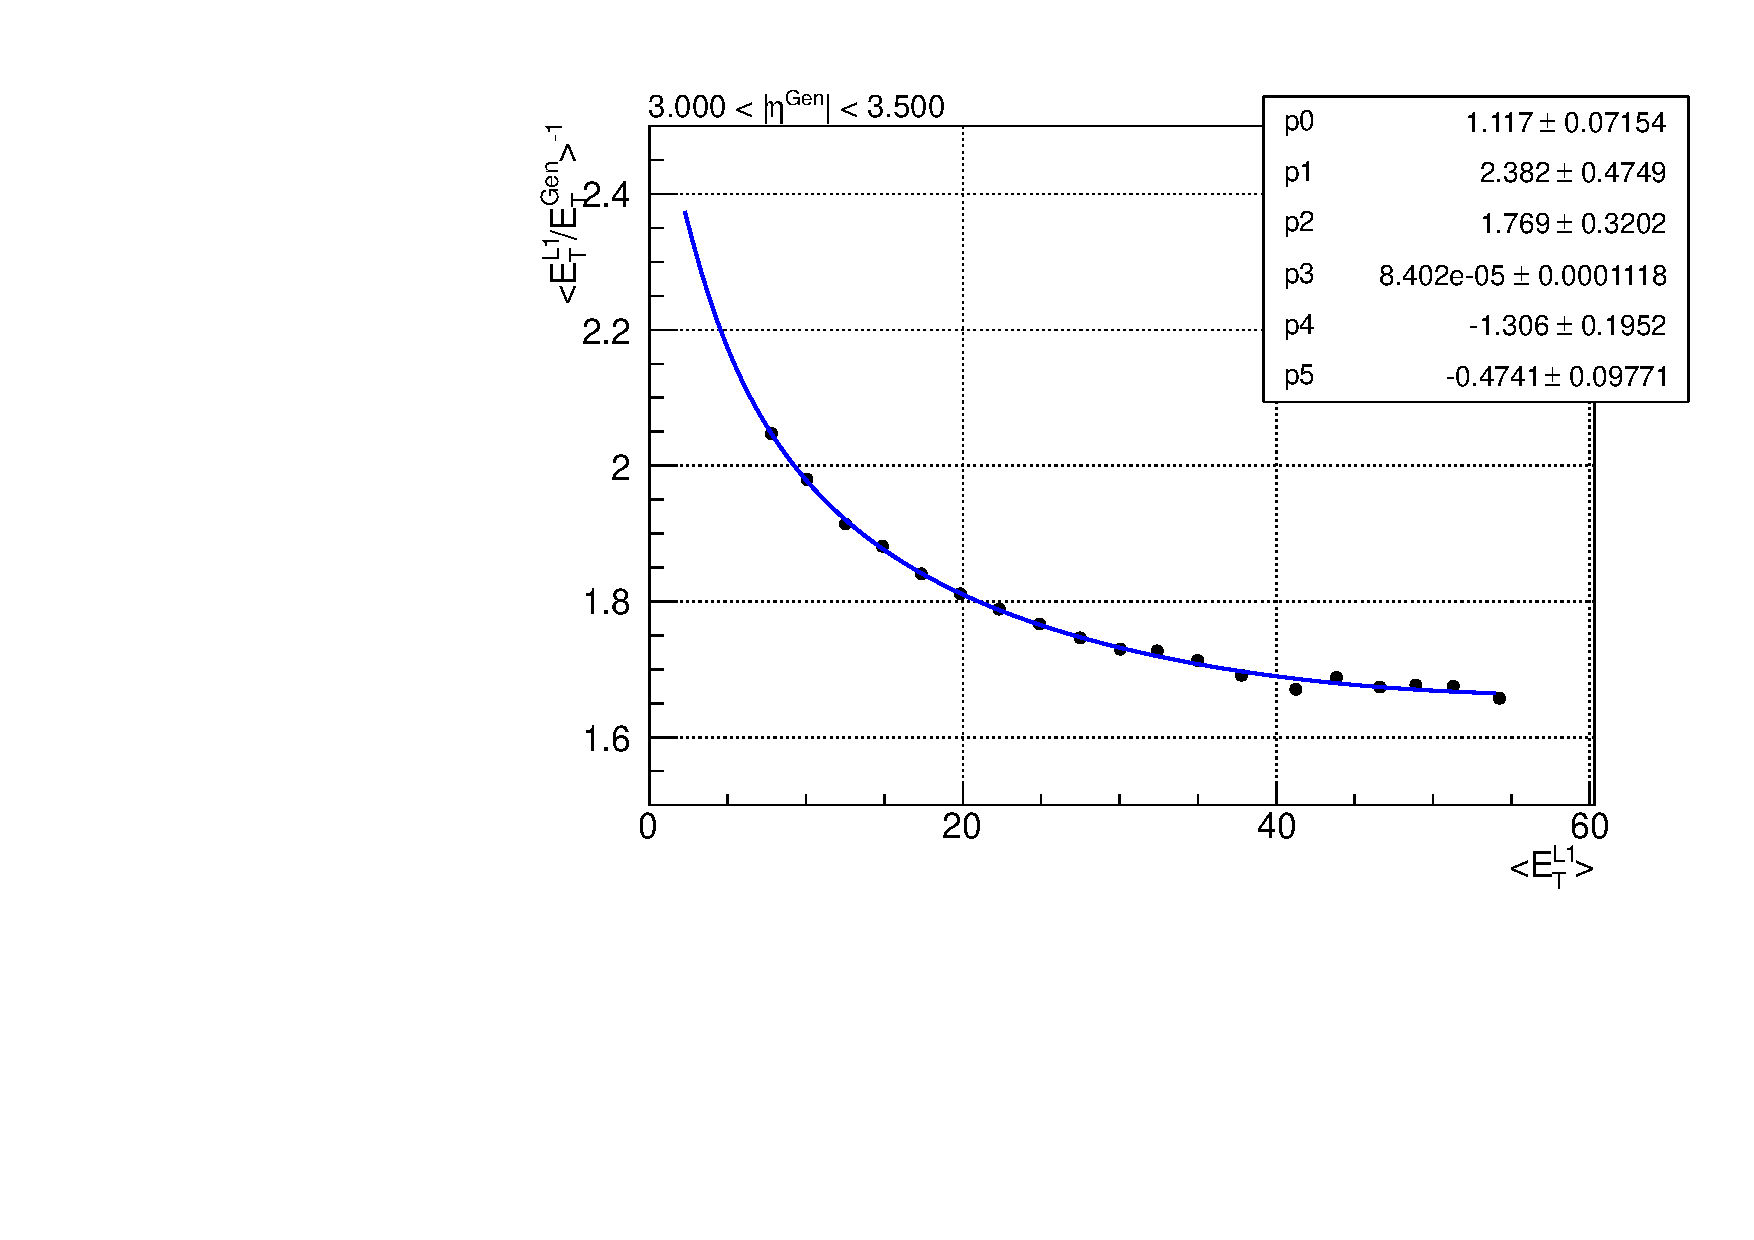
\includegraphics[width=0.49\textwidth]{detector/l1jet/egcor7.pdf}
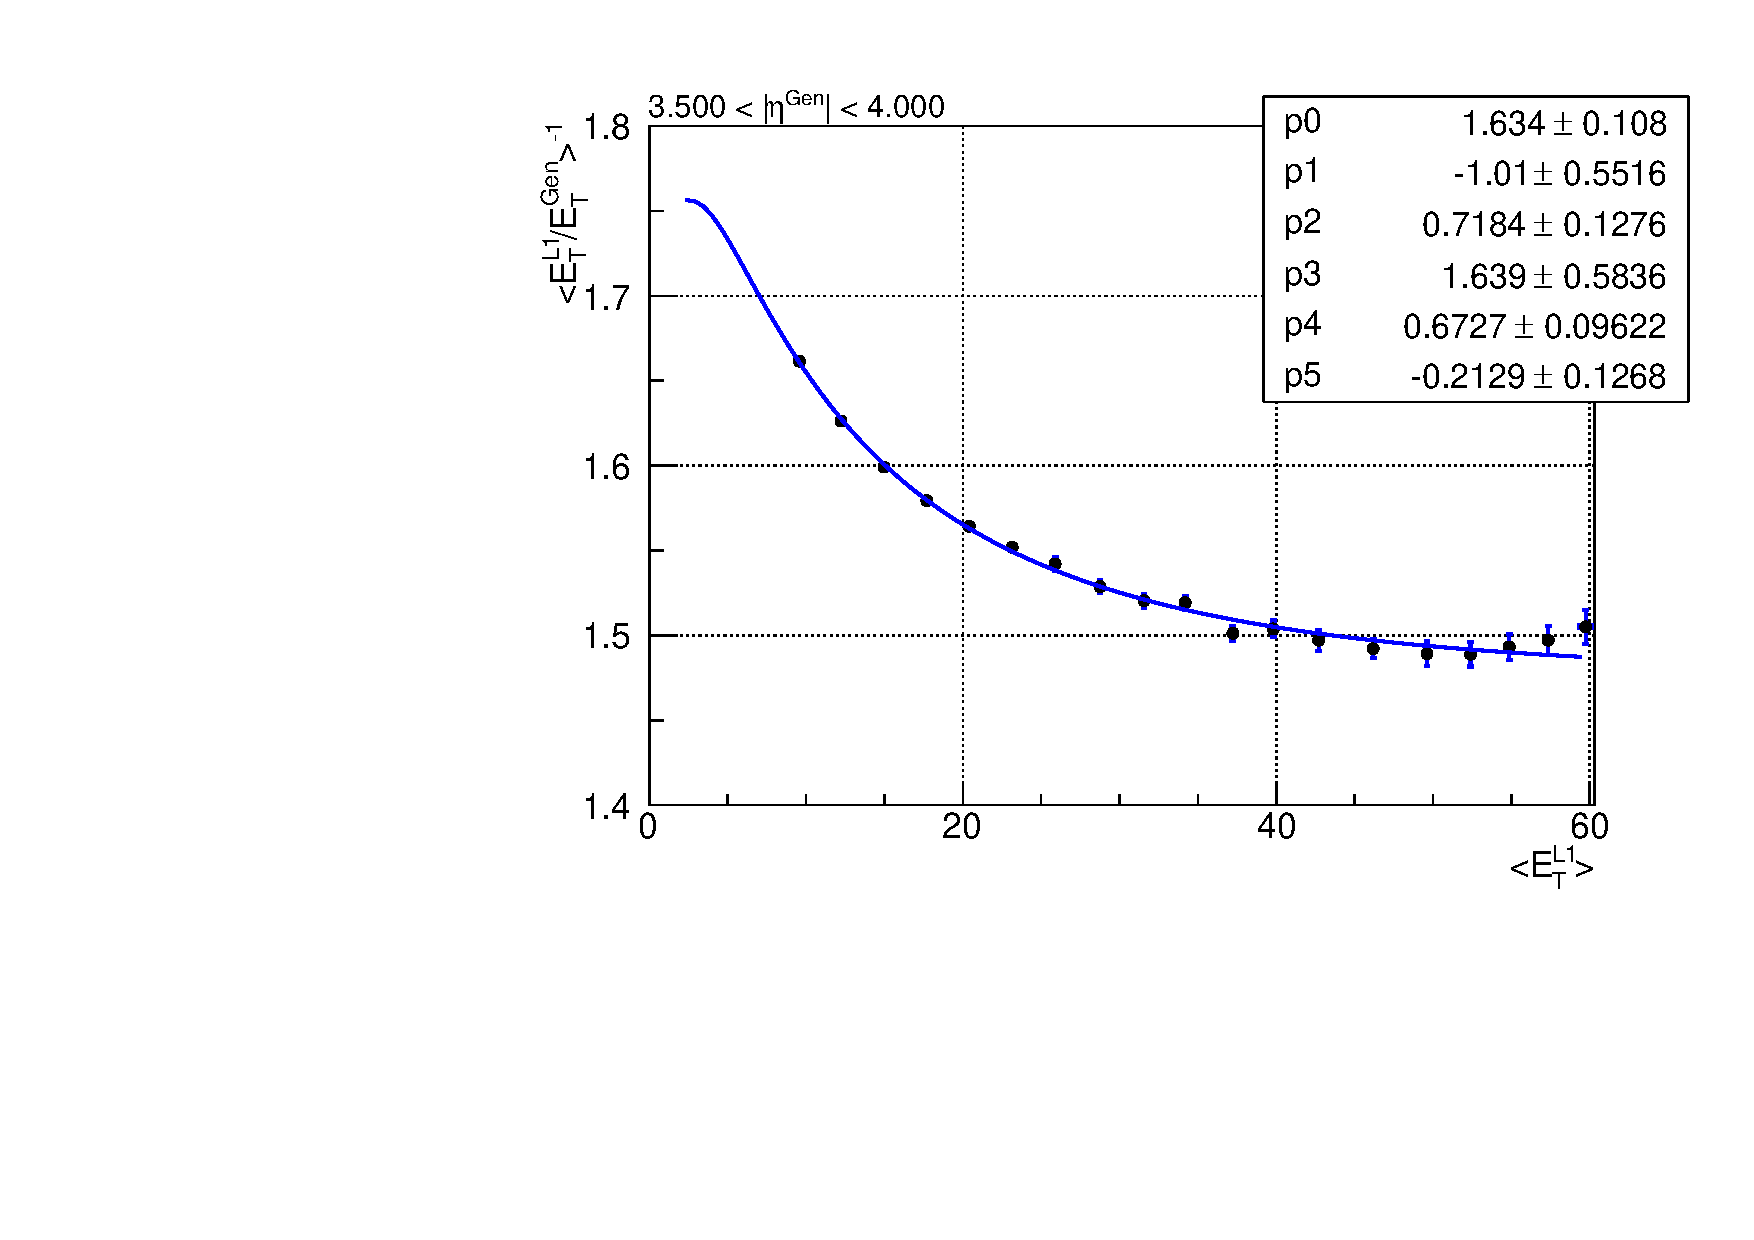
\includegraphics[width=0.49\textwidth]{detector/l1jet/egcor8.pdf}\\
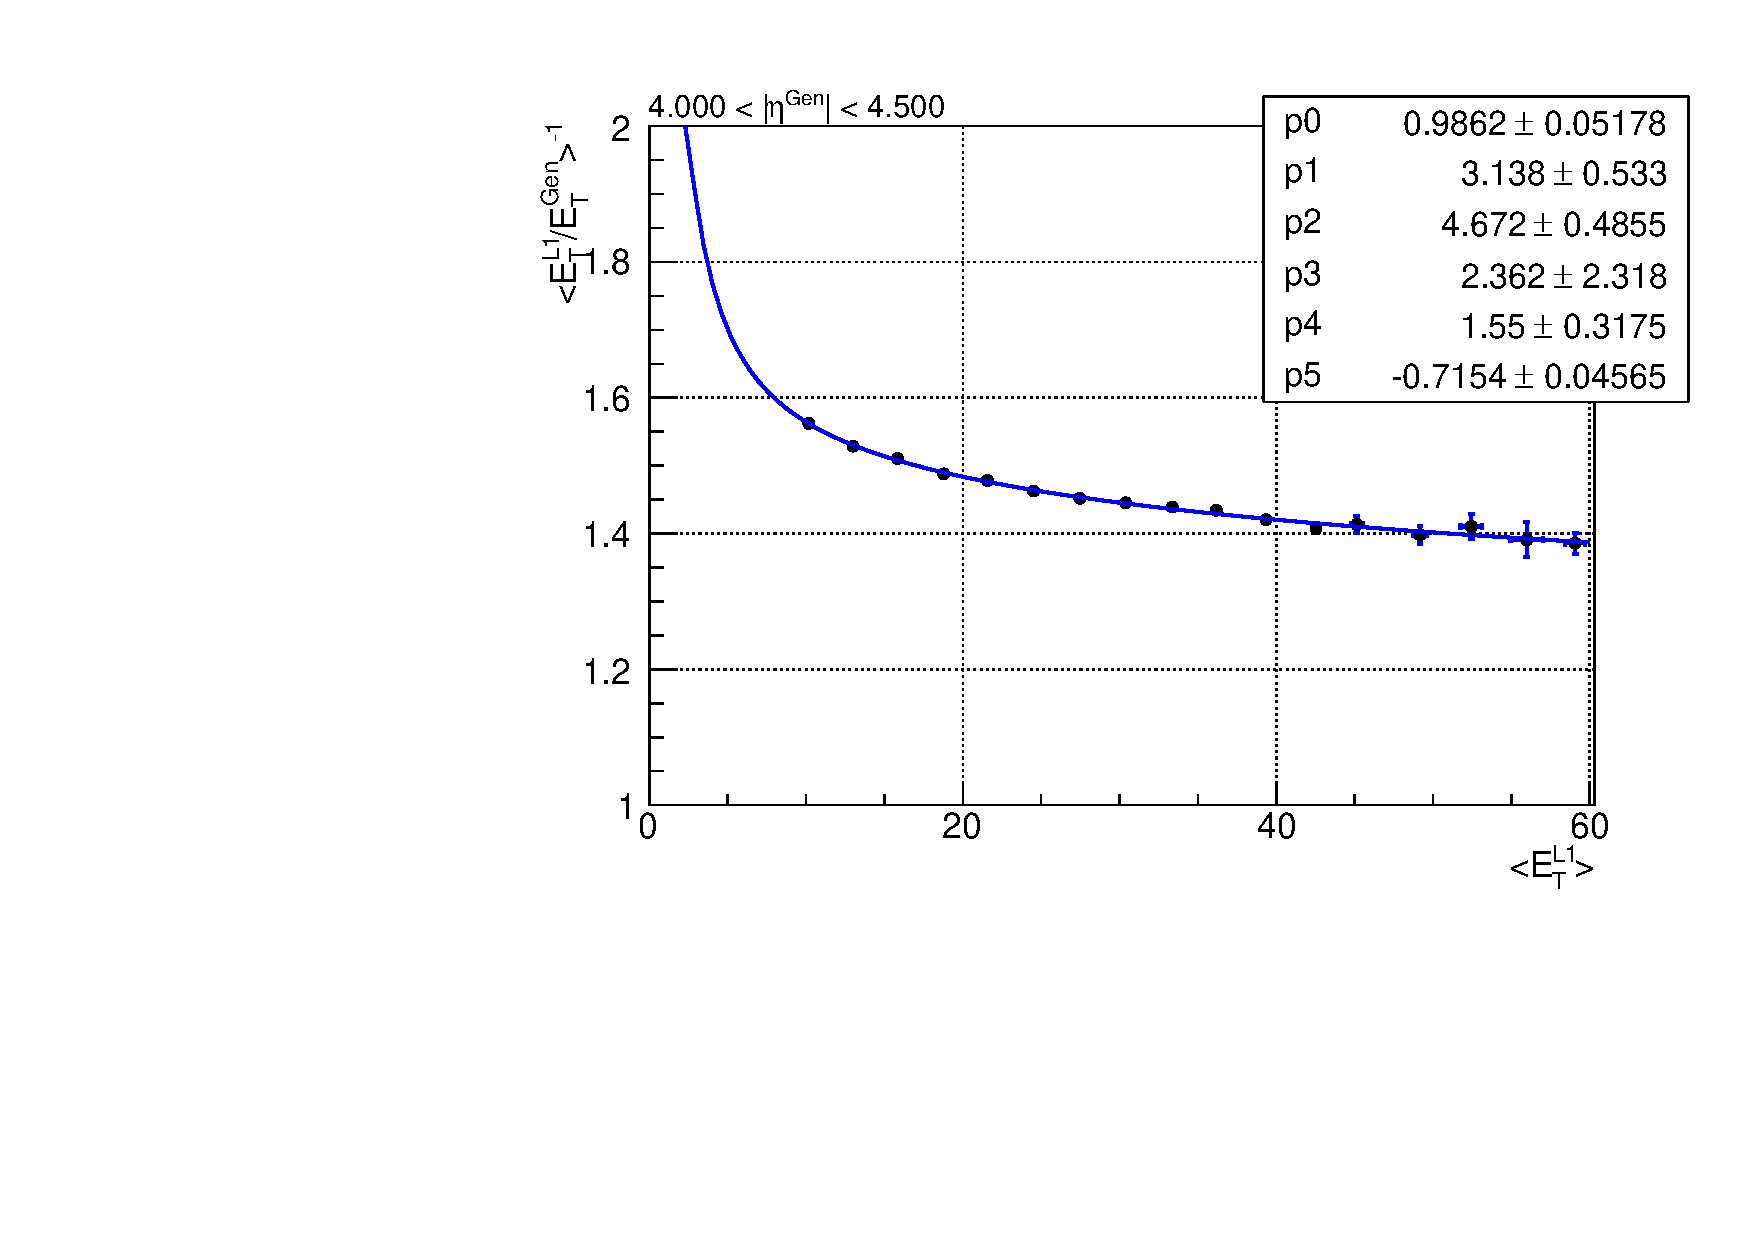
\includegraphics[width=0.49\textwidth]{detector/l1jet/egcor9.pdf}
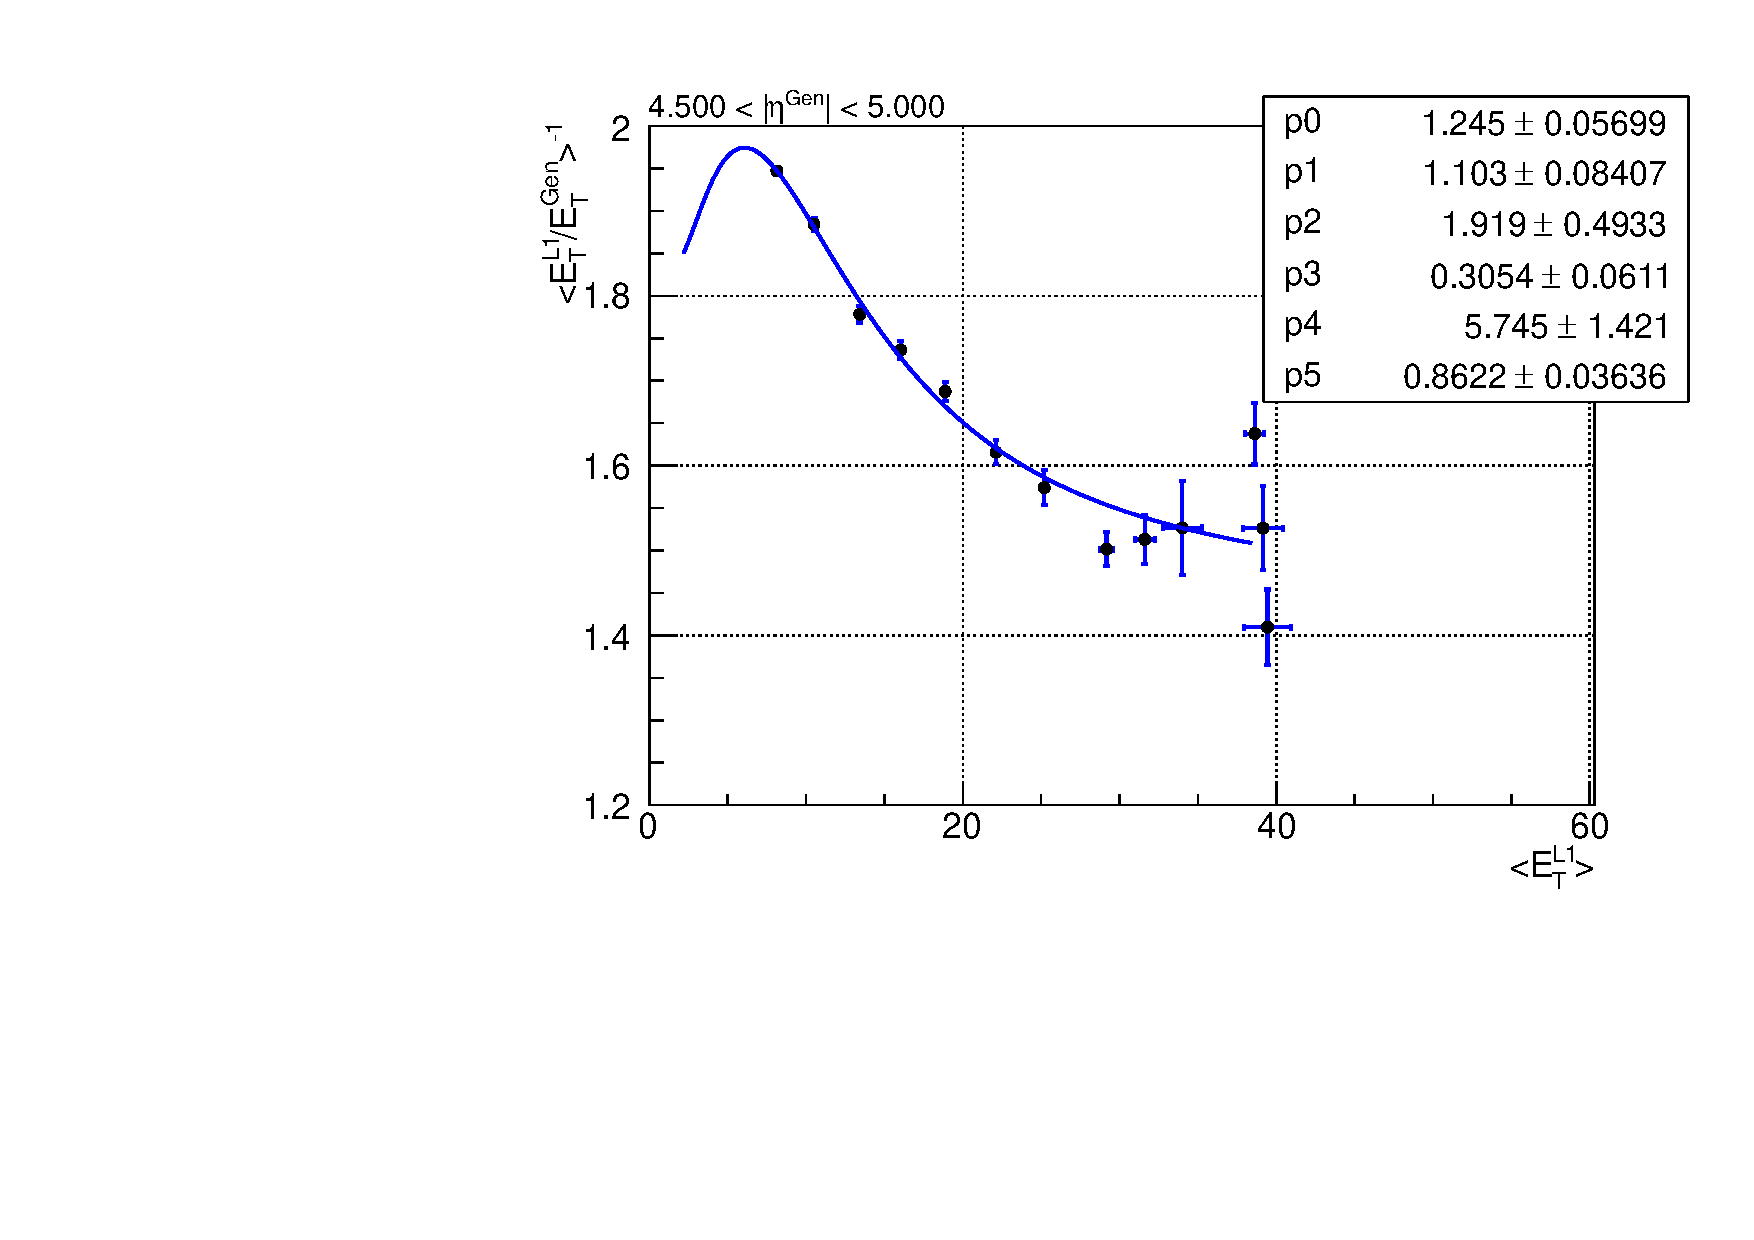
\includegraphics[width=0.49\textwidth]{detector/l1jet/egcor10.pdf}
\end{center}
\caption{Fitted correction functions for each of the 4 GCT regions covered by the HF. 
The points are fit with the function of Equation~\ref{eqn:jecfit} to 
provide a parameterisation of the corrections to be applied to 
jets online in the GCT.}
\label{fig:allcorrfuncsp2}
\end{figure}

\section{L1 Jet Resolution}
\label{app:closurefits}

The L1 jet resolution measured in MC was shown as a function of $\Lonept$ before and after applying
the derived jet energy calibrations in Figure~\ref{fig:mcresolutionl1}. The value of the response in at
each point is taken from a Gaussian fit to the distribution of $\Lonept/\Genpt$ in bins of $\Lonept$.
Figures~\ref{fig:mcresfits_u_p1} and~\ref{fig:mcresfits_u_p2} show the fits before applying the corrections while
Figures~\ref{fig:mcresfits_pf_p1} and~\ref{fig:mcresfits_pf_p2} show the fits after.
The central value for the points in Figure~\ref{fig:mcresolutionl1} are taken from the width ($\sigma$) of the fitted Gaussian 
distributions. The error bars on this plot are taken from the error on the fitted value of $\sigma$ which is too small to be visible.
The improvement in resolution after applying the corrections is clearly visible.
\begin{figure}[h!]
    \centering
          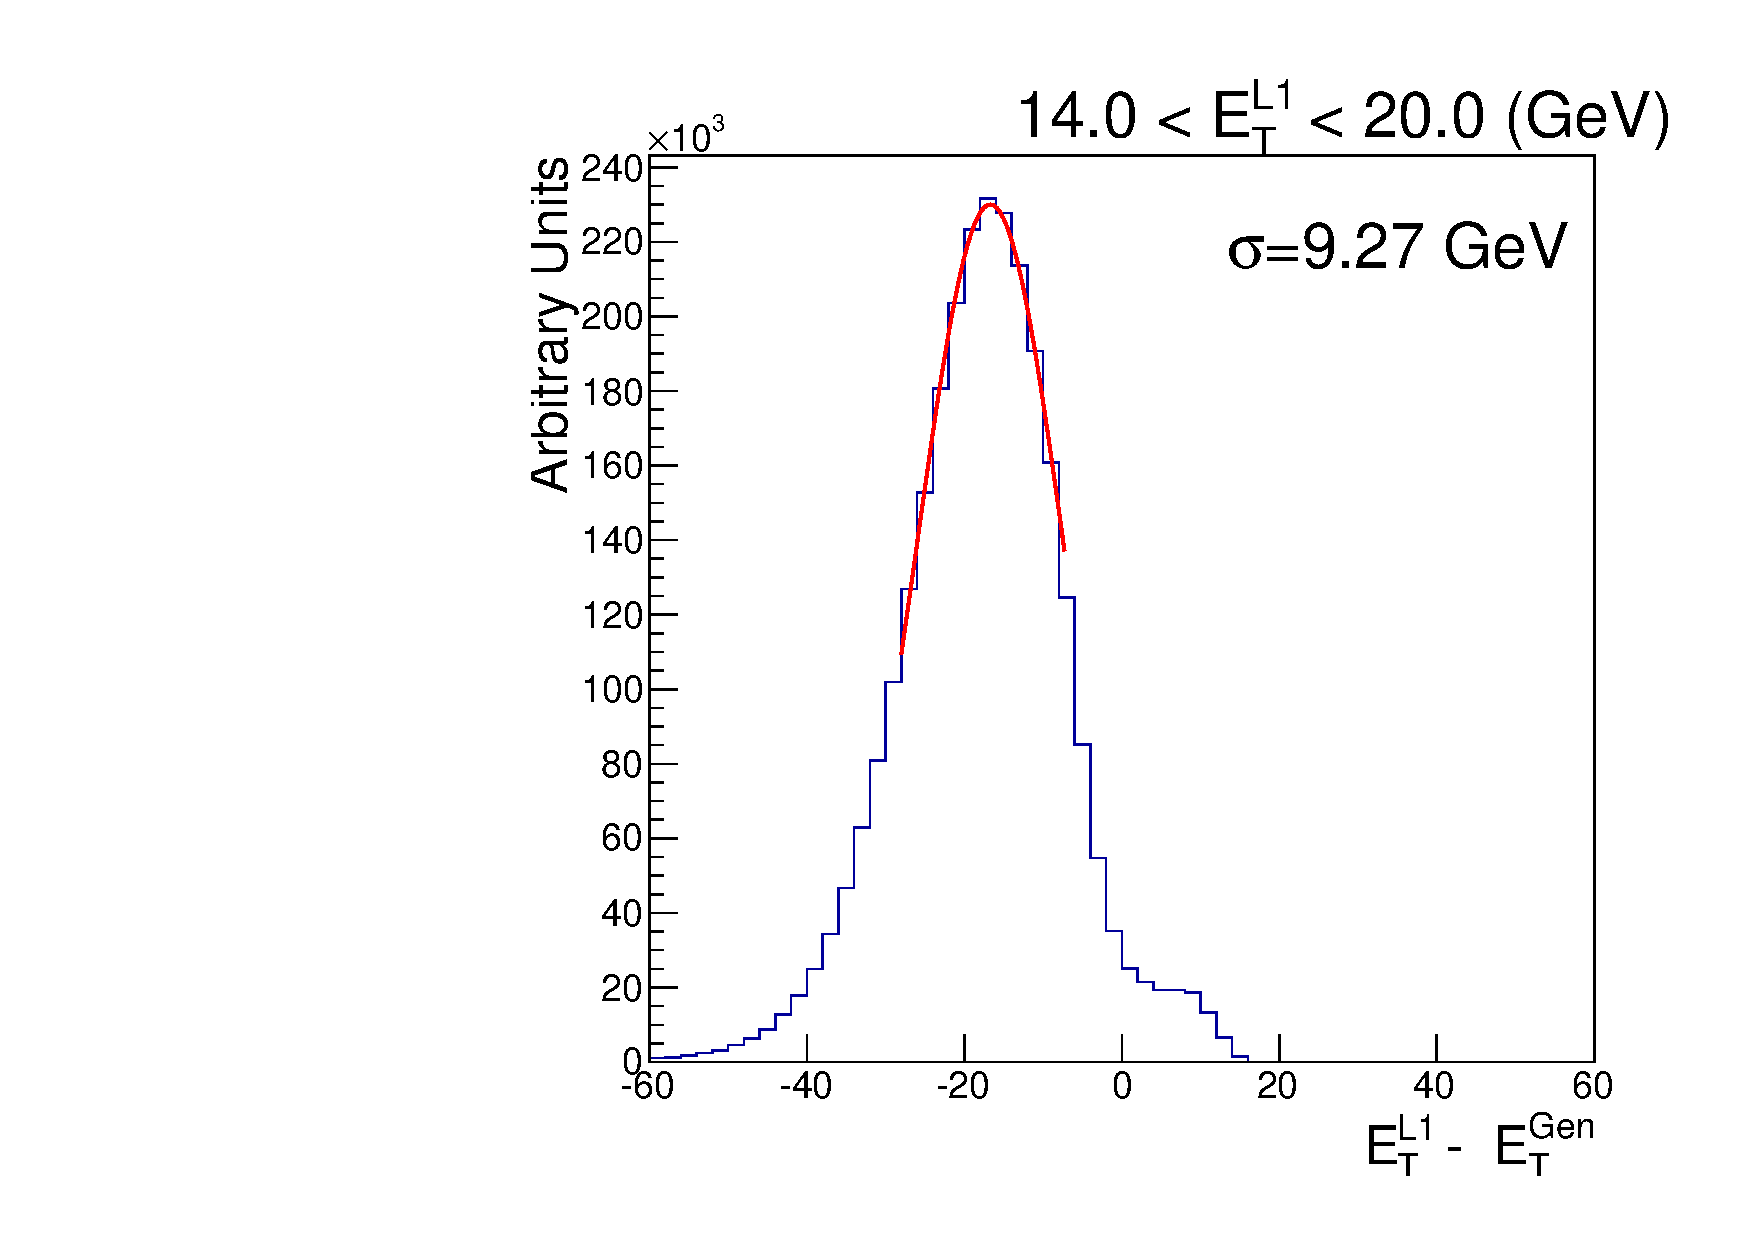
\includegraphics[width=0.32\textwidth]{detector/l1jet/gaussfits//ptBin_0_PtAll_u.pdf}
          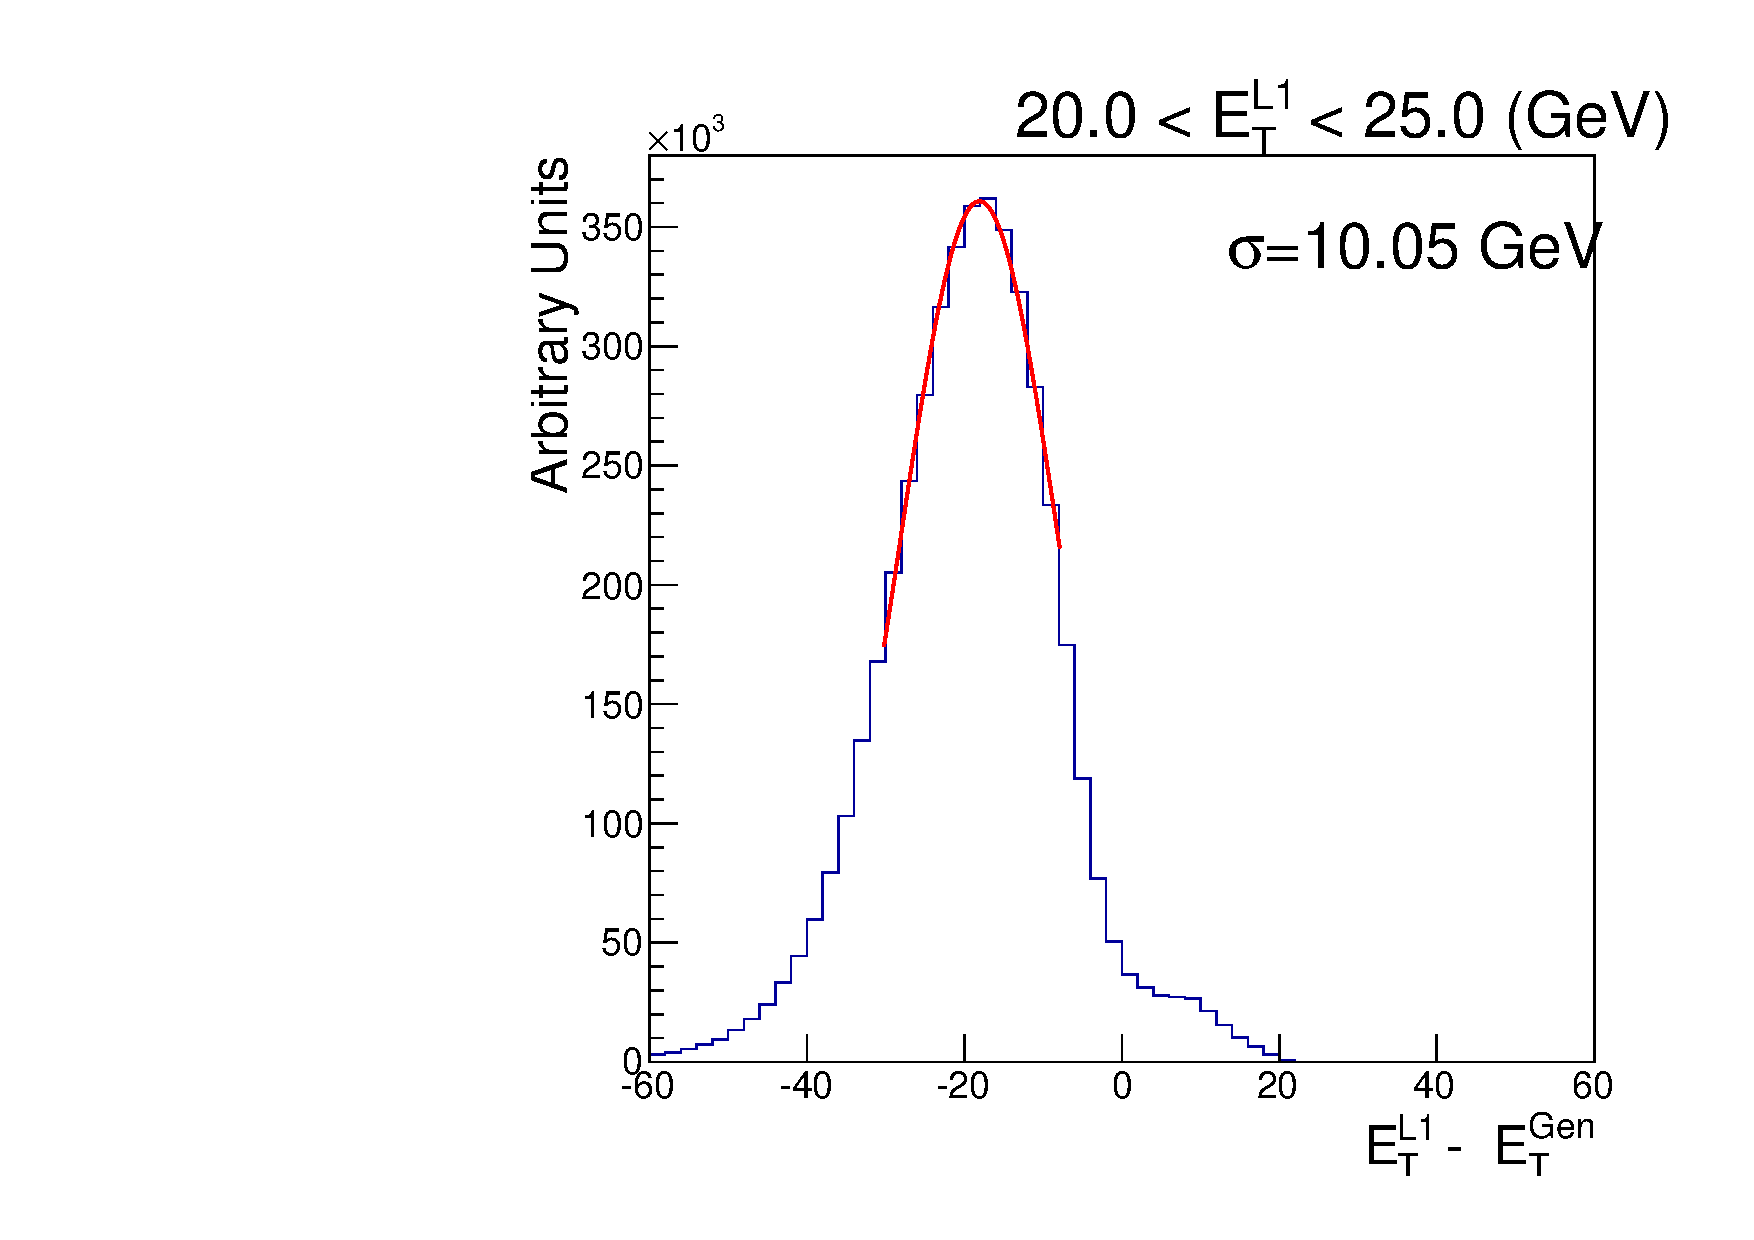
\includegraphics[width=0.32\textwidth]{detector/l1jet/gaussfits//ptBin_1_PtAll_u.pdf}
          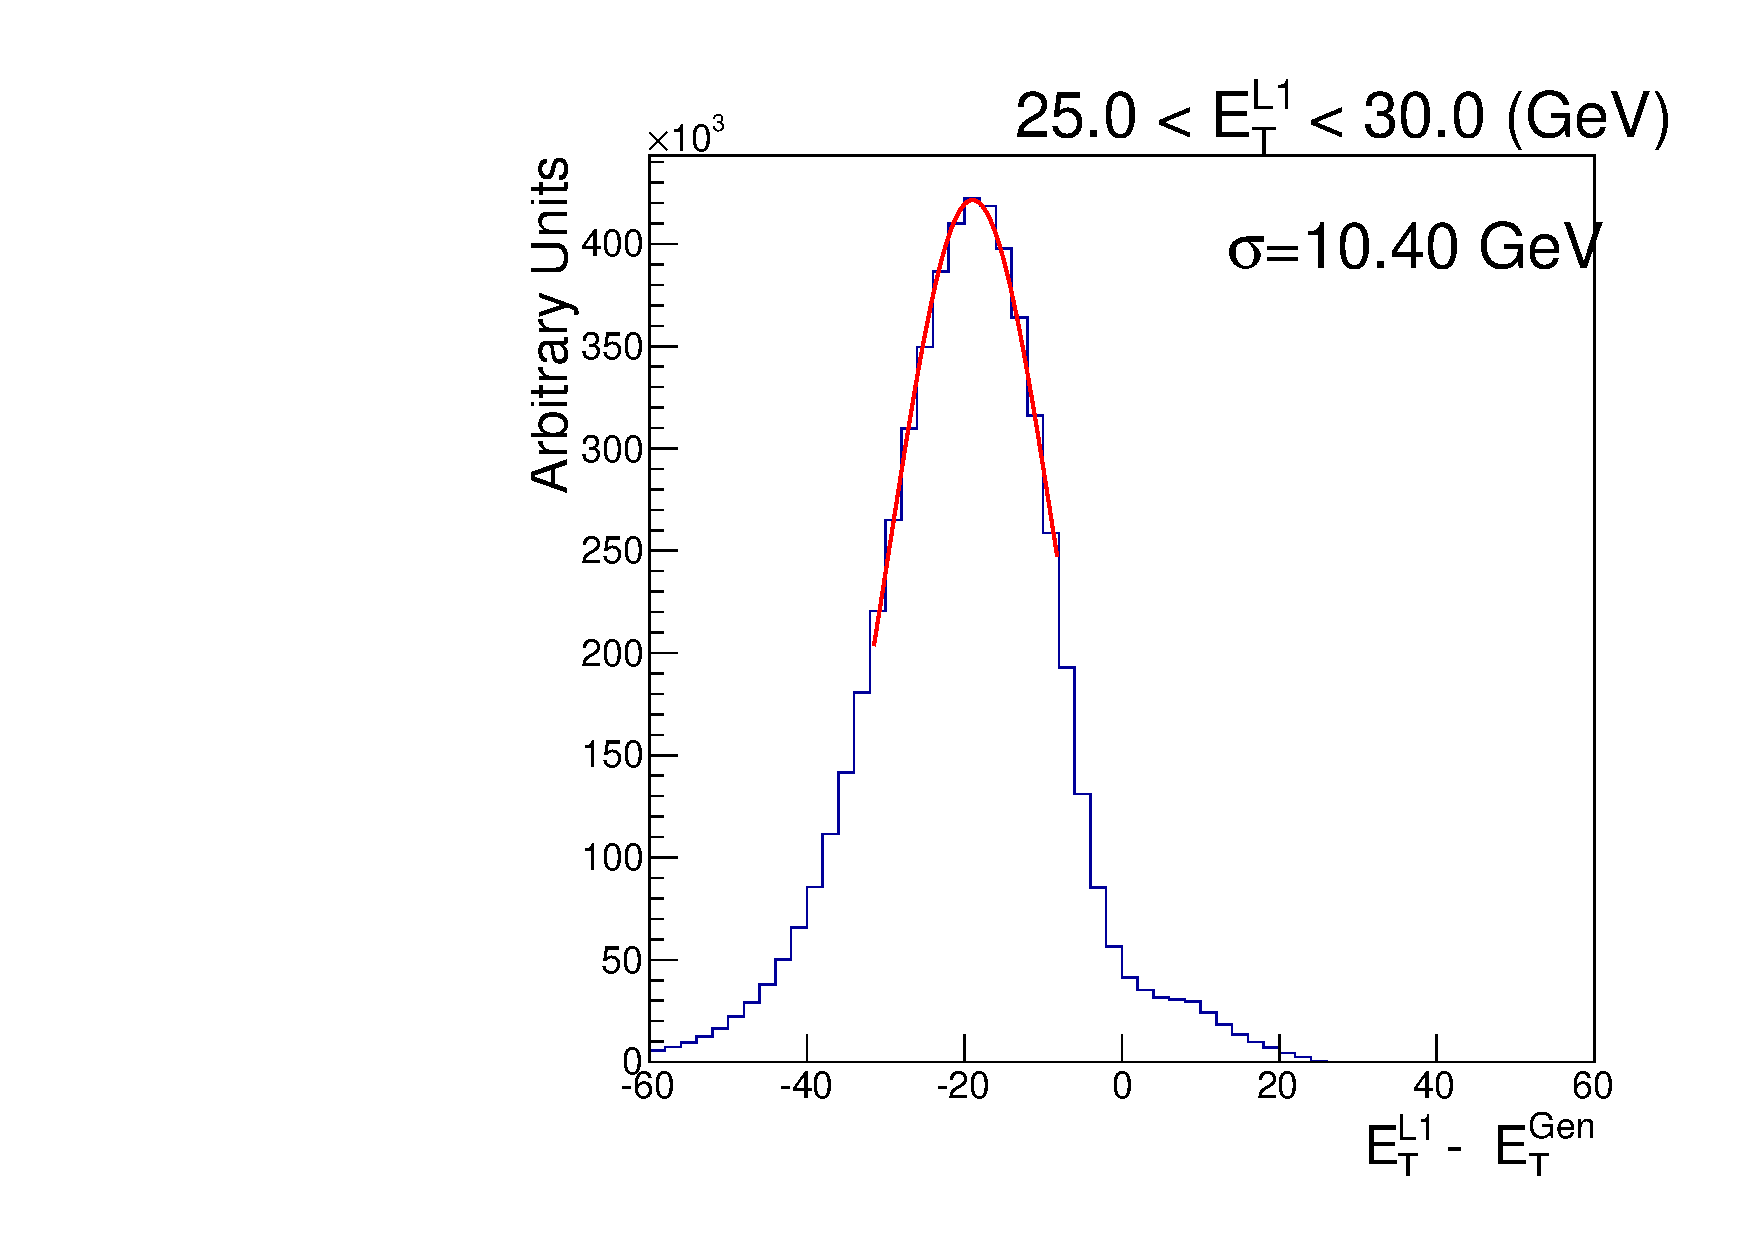
\includegraphics[width=0.32\textwidth]{detector/l1jet/gaussfits//ptBin_2_PtAll_u.pdf}\\
          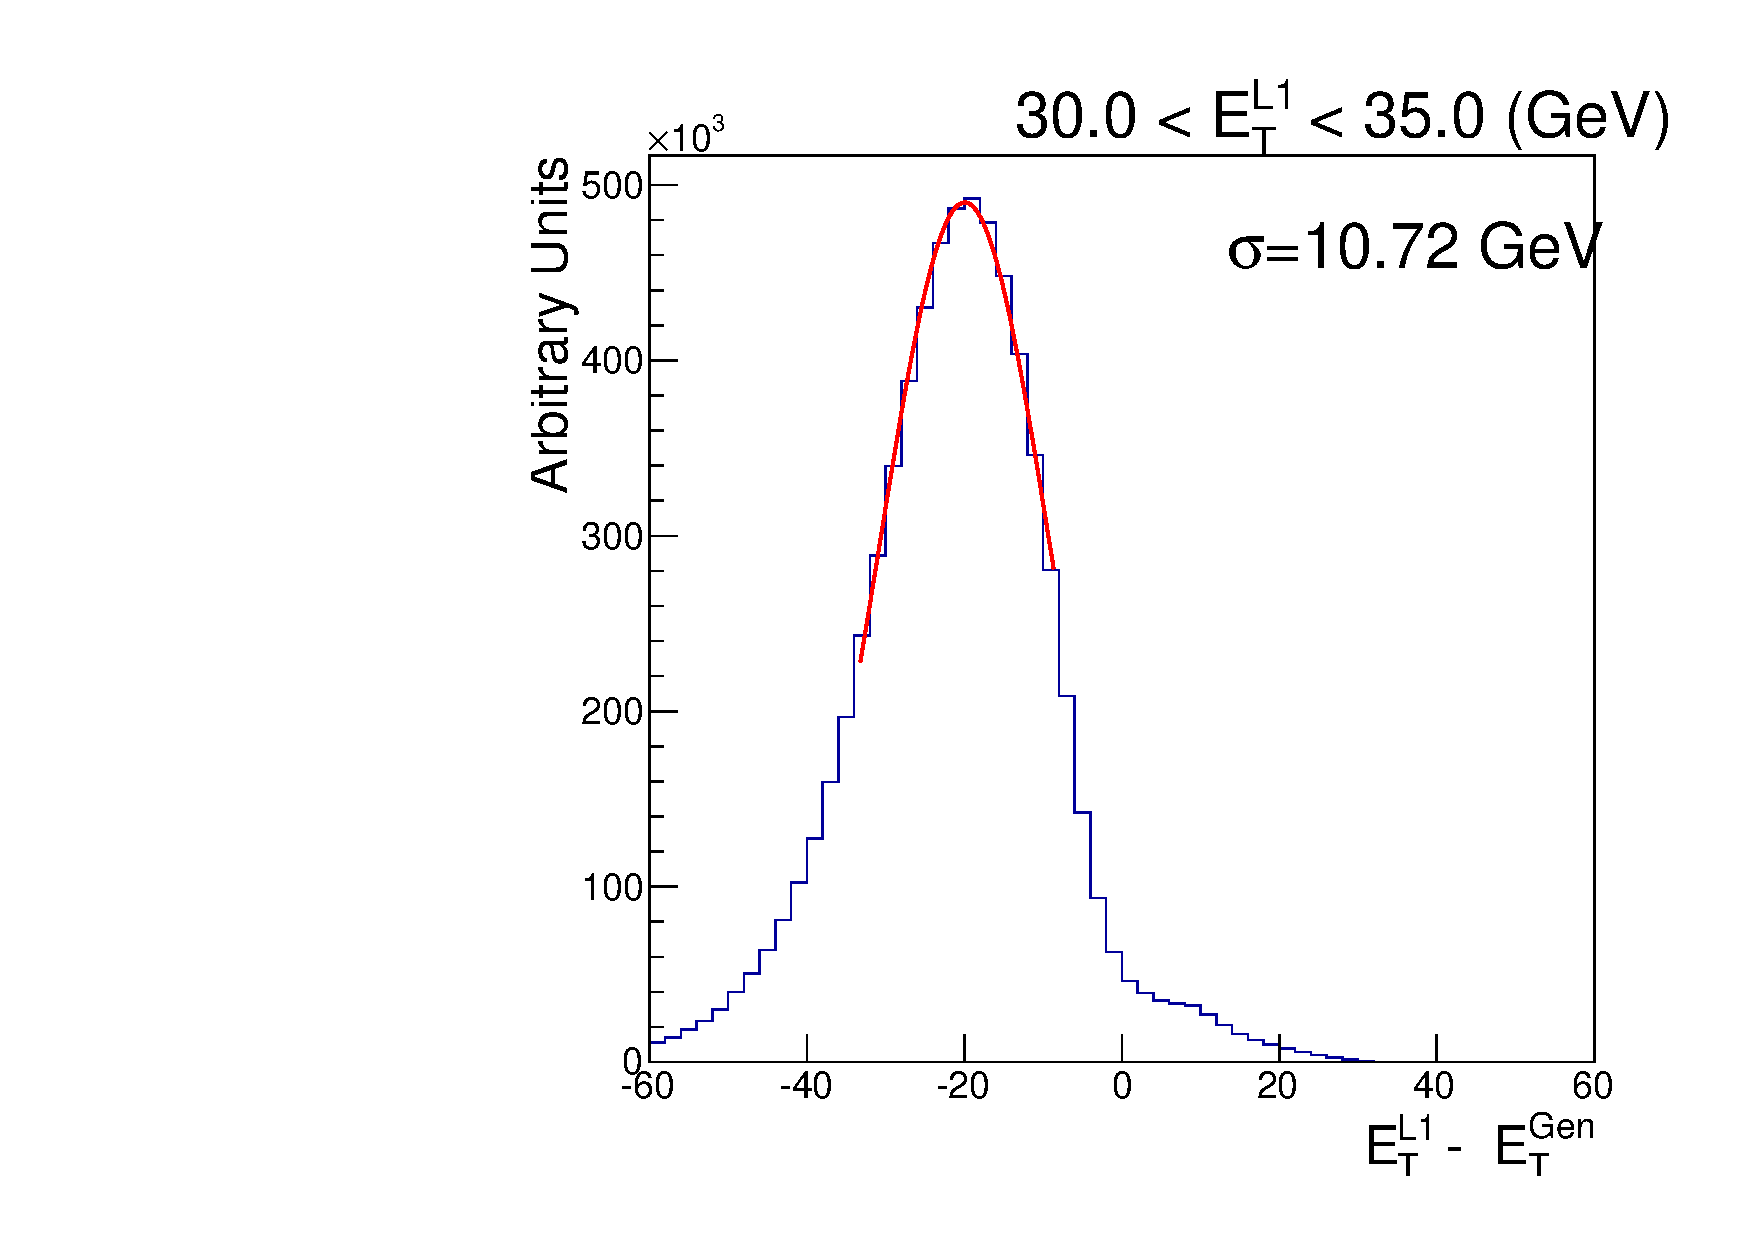
\includegraphics[width=0.32\textwidth]{detector/l1jet/gaussfits//ptBin_3_PtAll_u.pdf}
          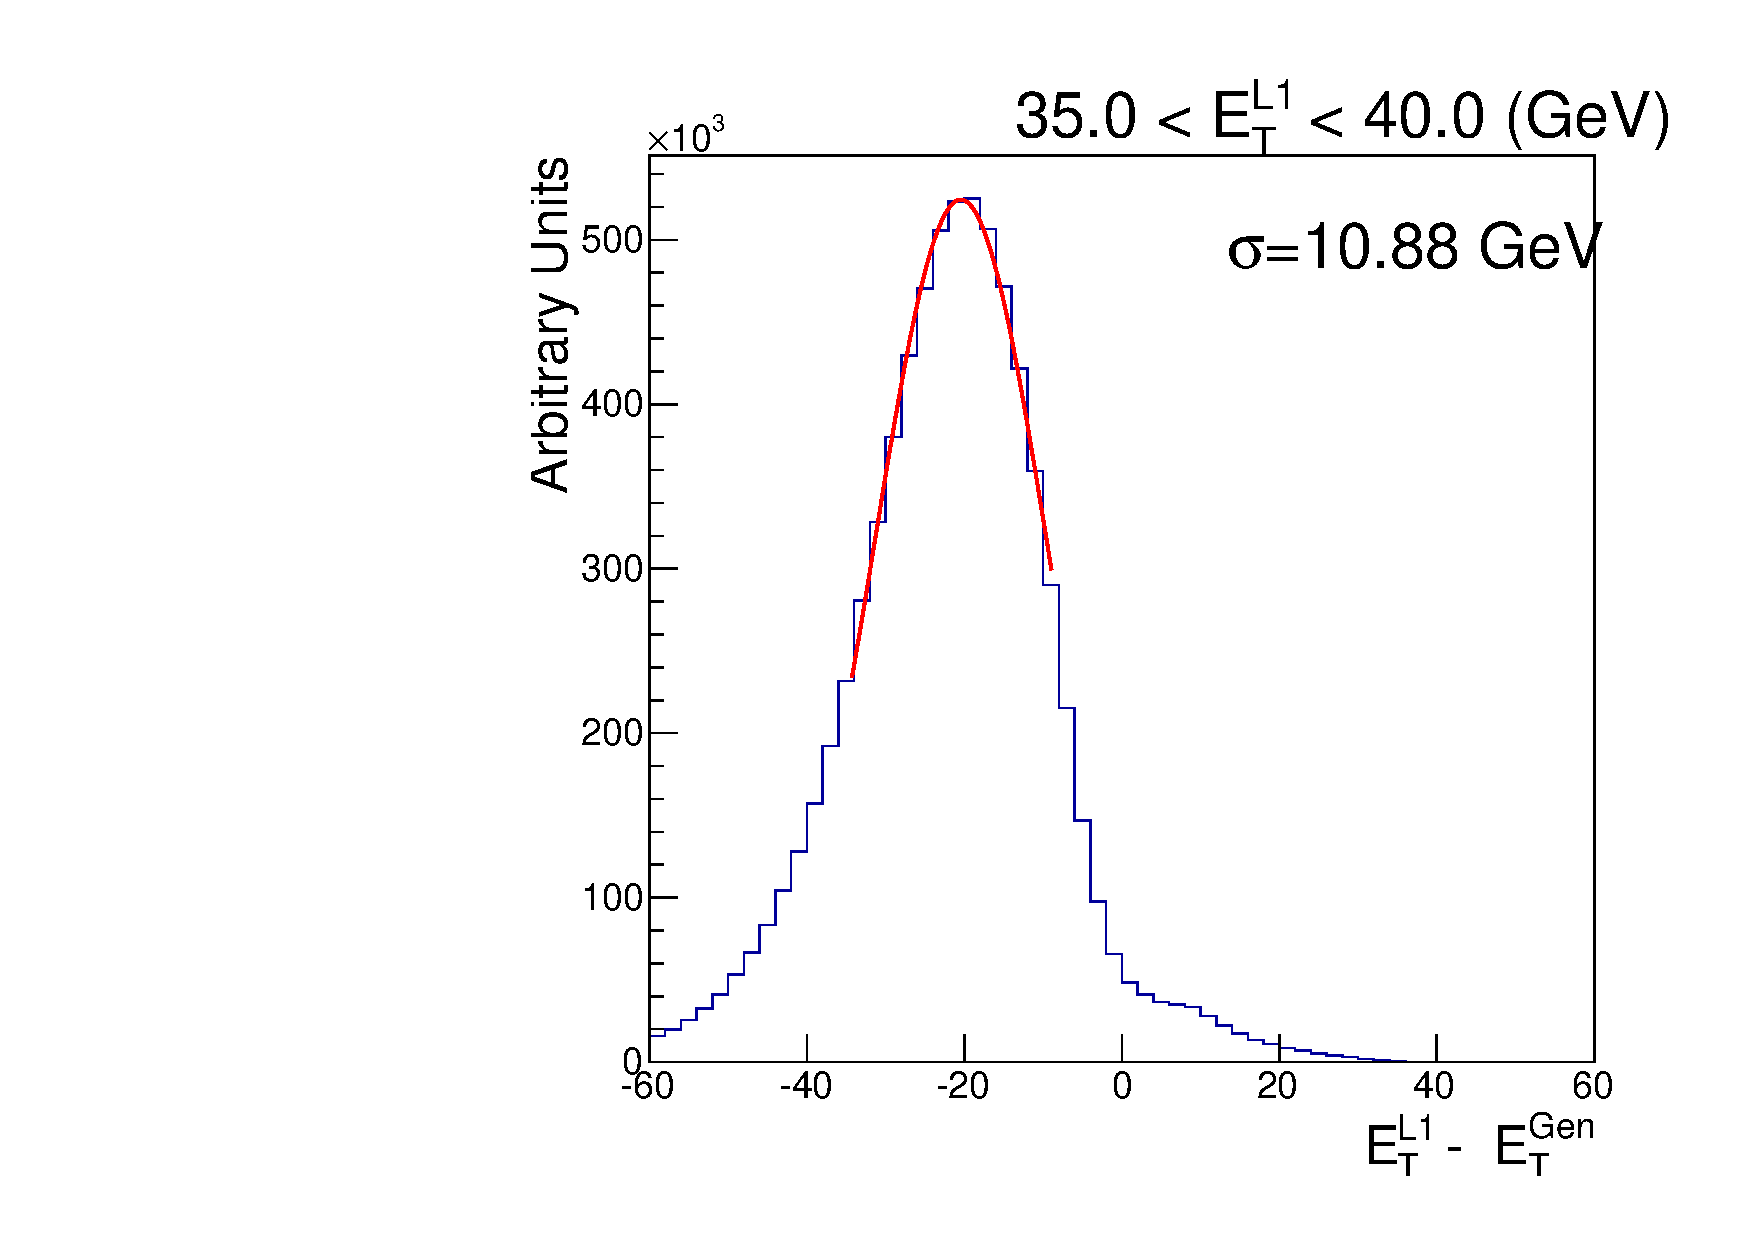
\includegraphics[width=0.32\textwidth]{detector/l1jet/gaussfits//ptBin_4_PtAll_u.pdf}
          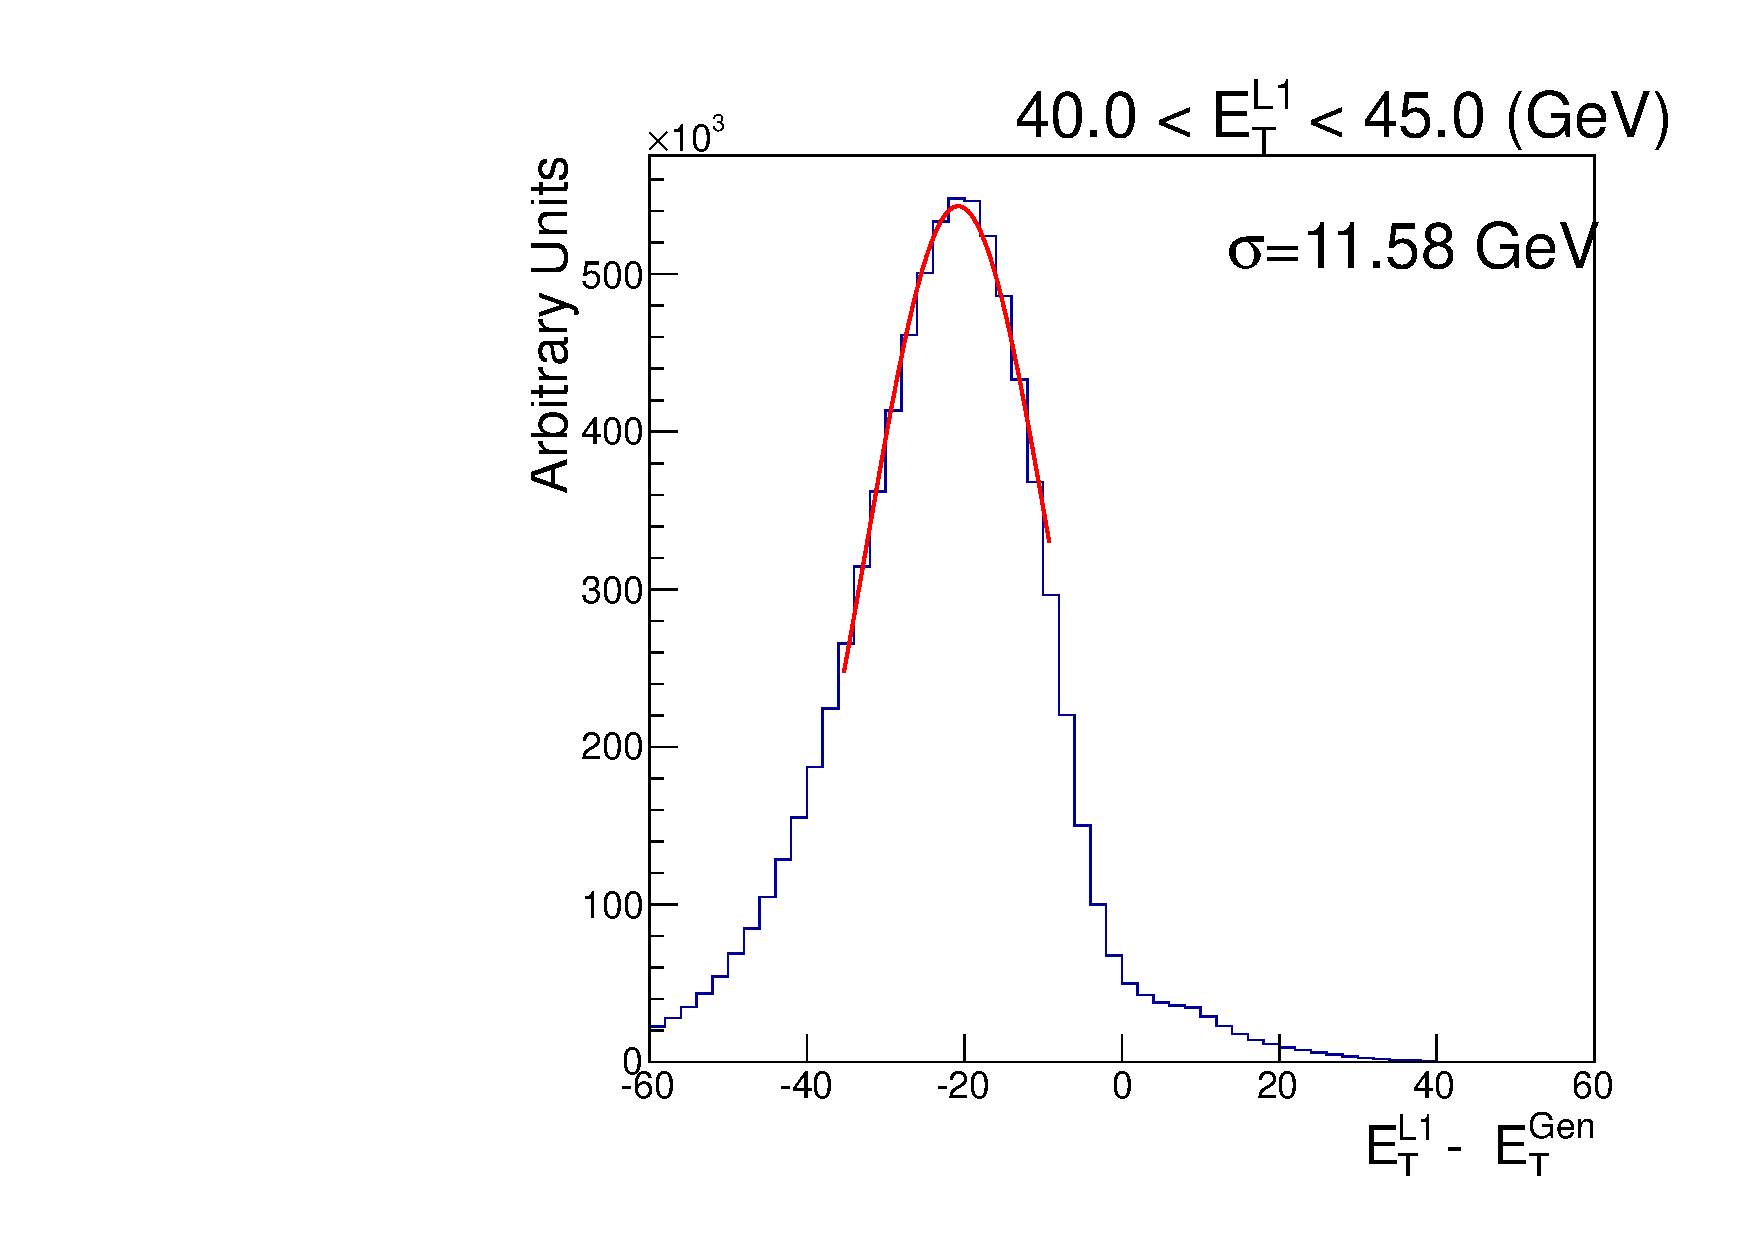
\includegraphics[width=0.32\textwidth]{detector/l1jet/gaussfits//ptBin_5_PtAll_u.pdf}\\
          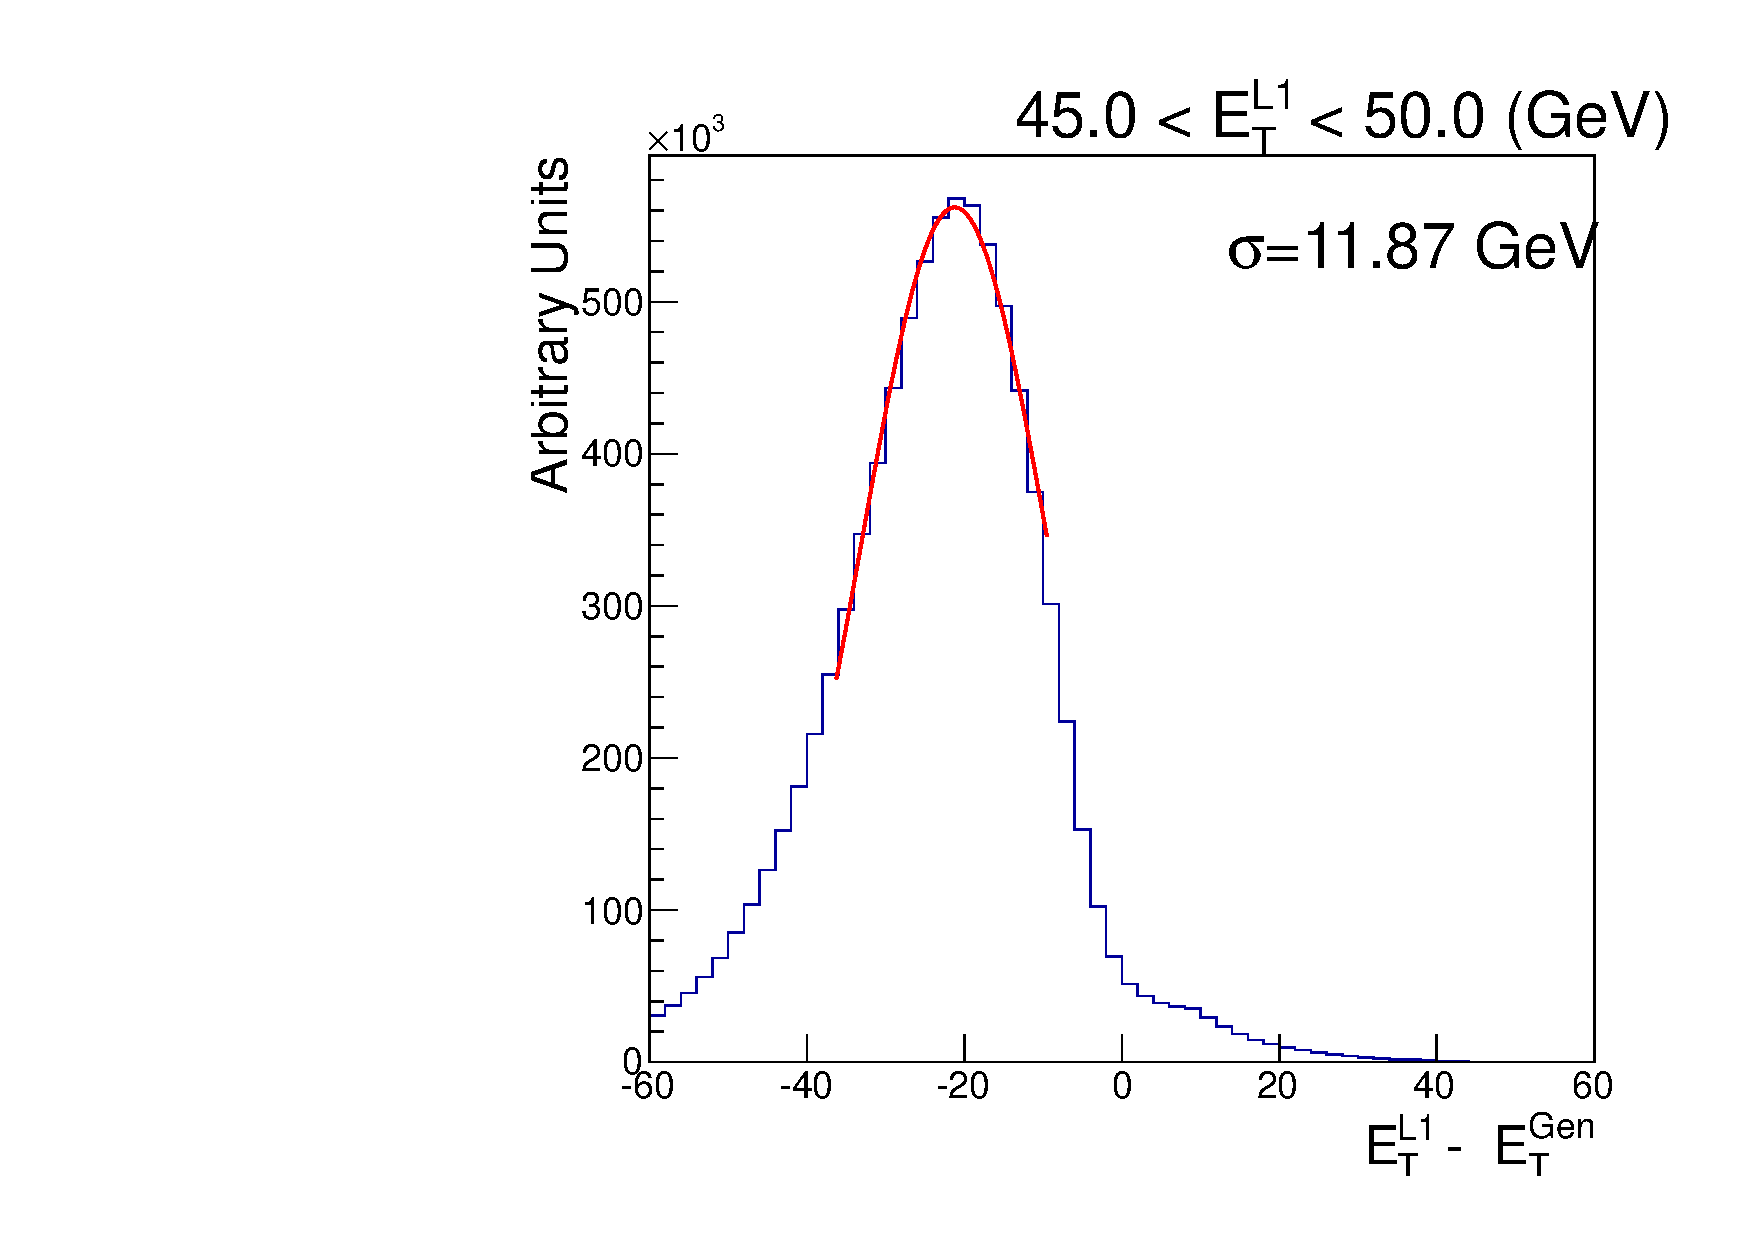
\includegraphics[width=0.32\textwidth]{detector/l1jet/gaussfits//ptBin_6_PtAll_u.pdf}
    \caption{Part one of the distributions of $\Lonept-\Genpt$ in bins of $\Lonept$ of the uncorrected MC jets. 
	The fitted Gaussian is used to extract the resolution as a function of $\Lonept$.}
    \label{fig:mcresfits_u_p1}
\end{figure}

\begin{figure}[h!]
    \centering
          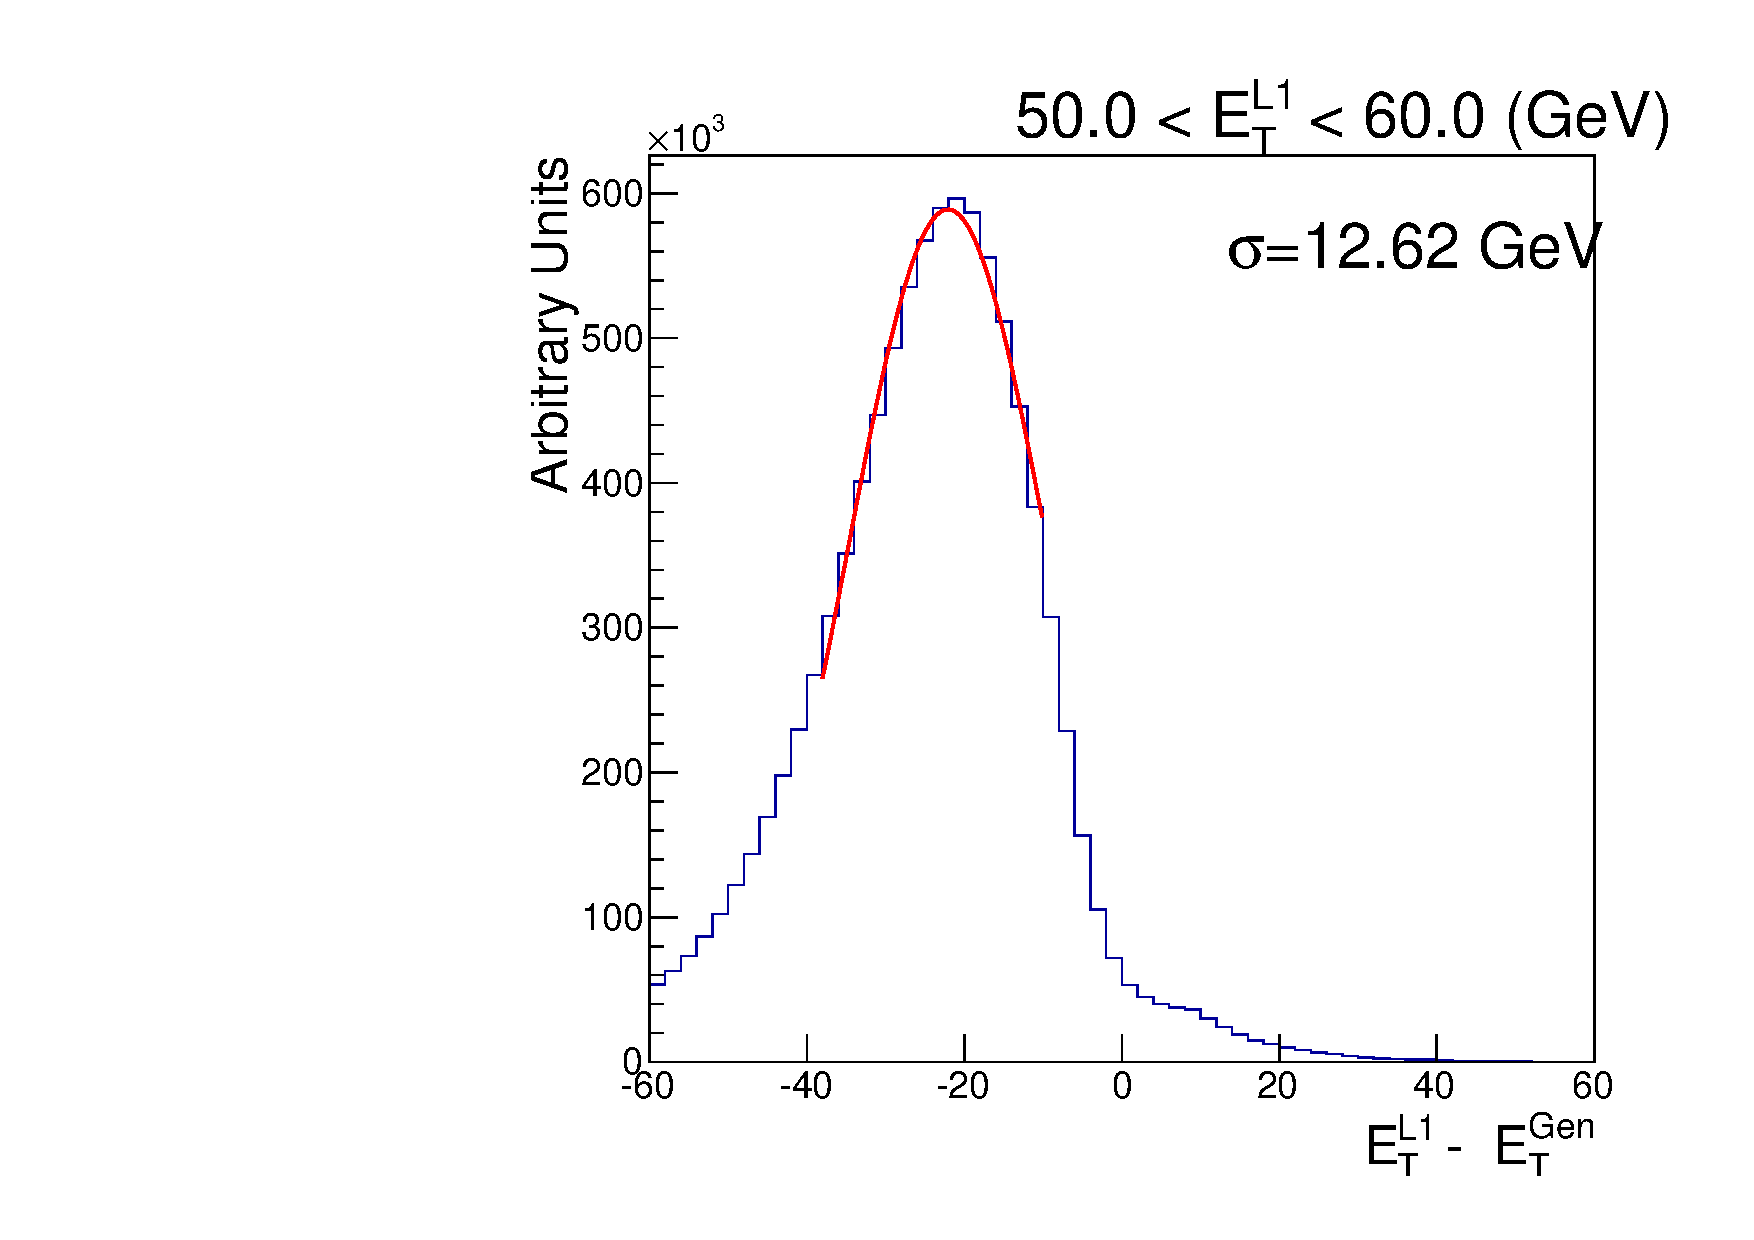
\includegraphics[width=0.32\textwidth]{detector/l1jet/gaussfits//ptBin_7_PtAll_u.pdf}
          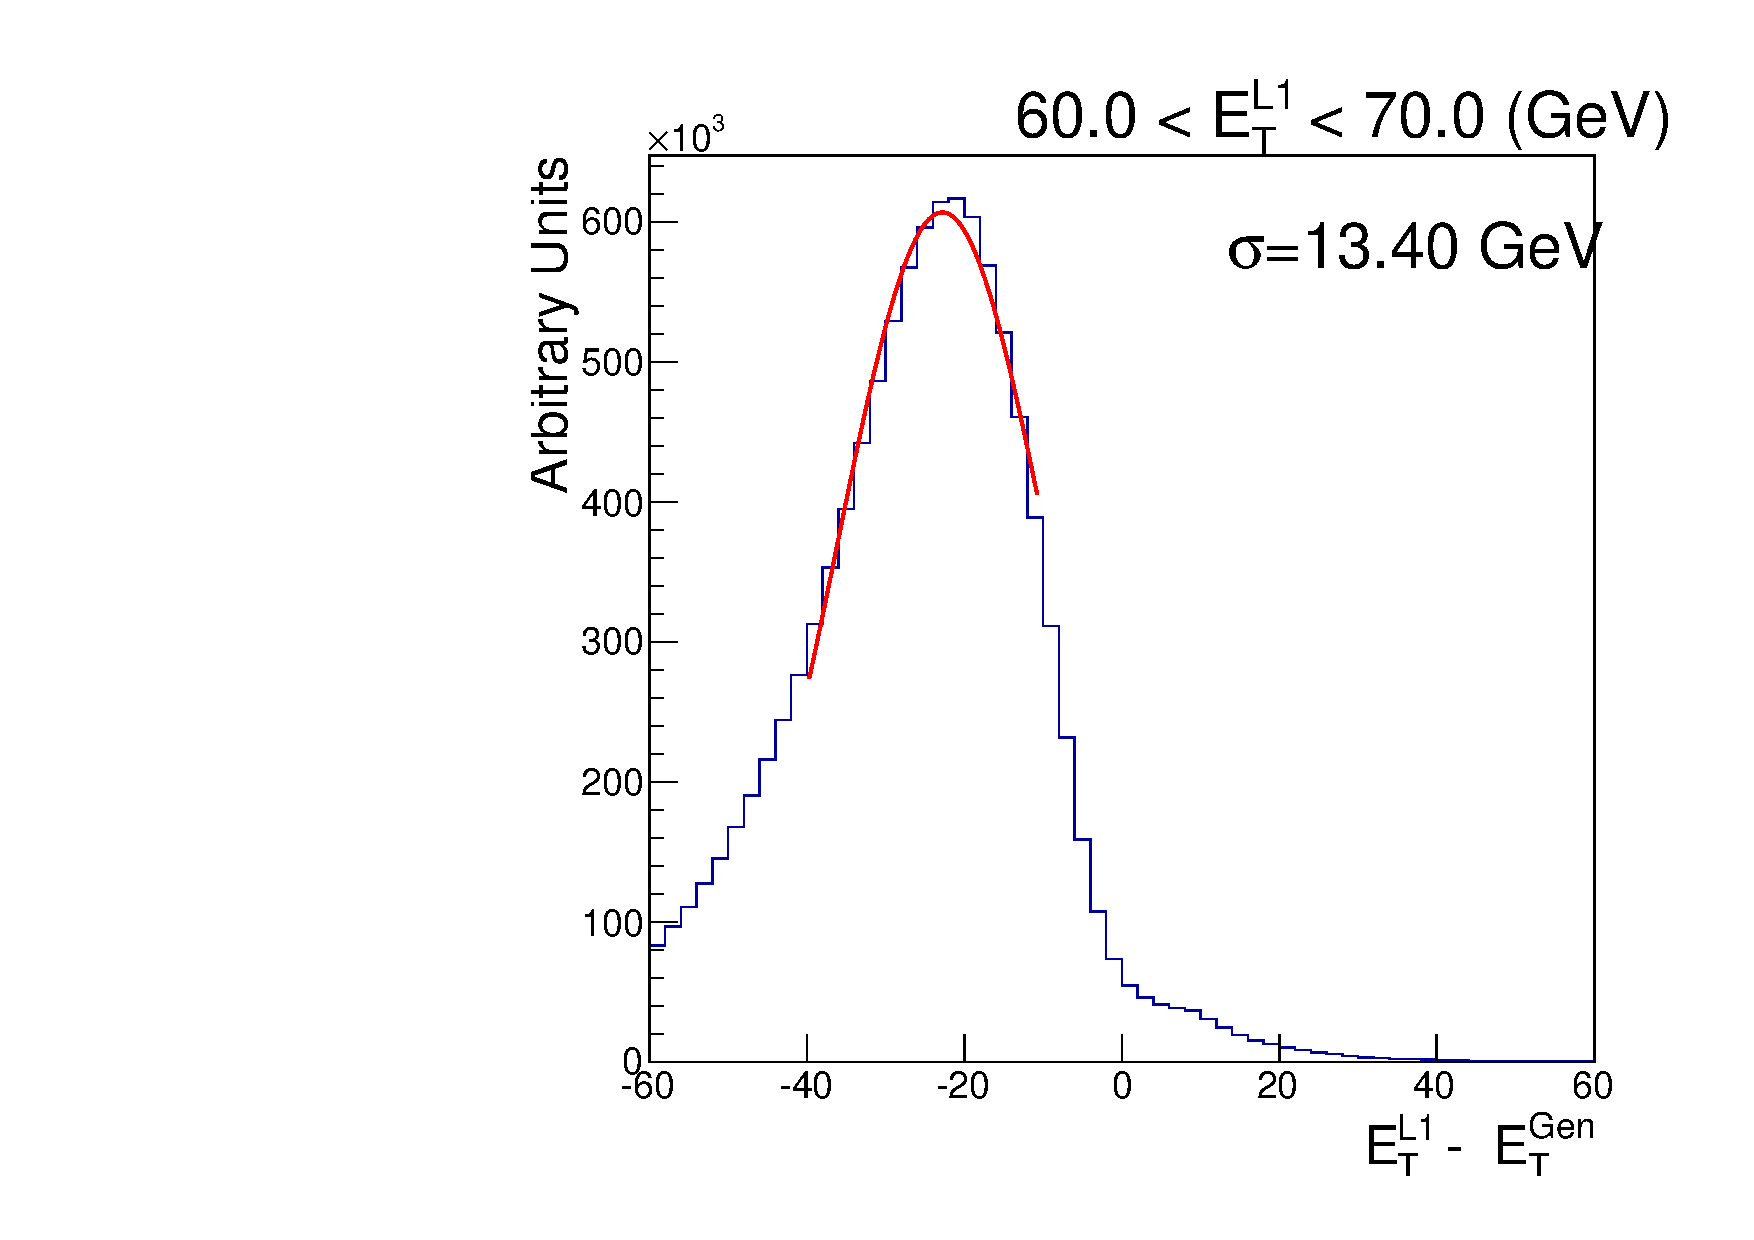
\includegraphics[width=0.32\textwidth]{detector/l1jet/gaussfits//ptBin_8_PtAll_u.pdf}
          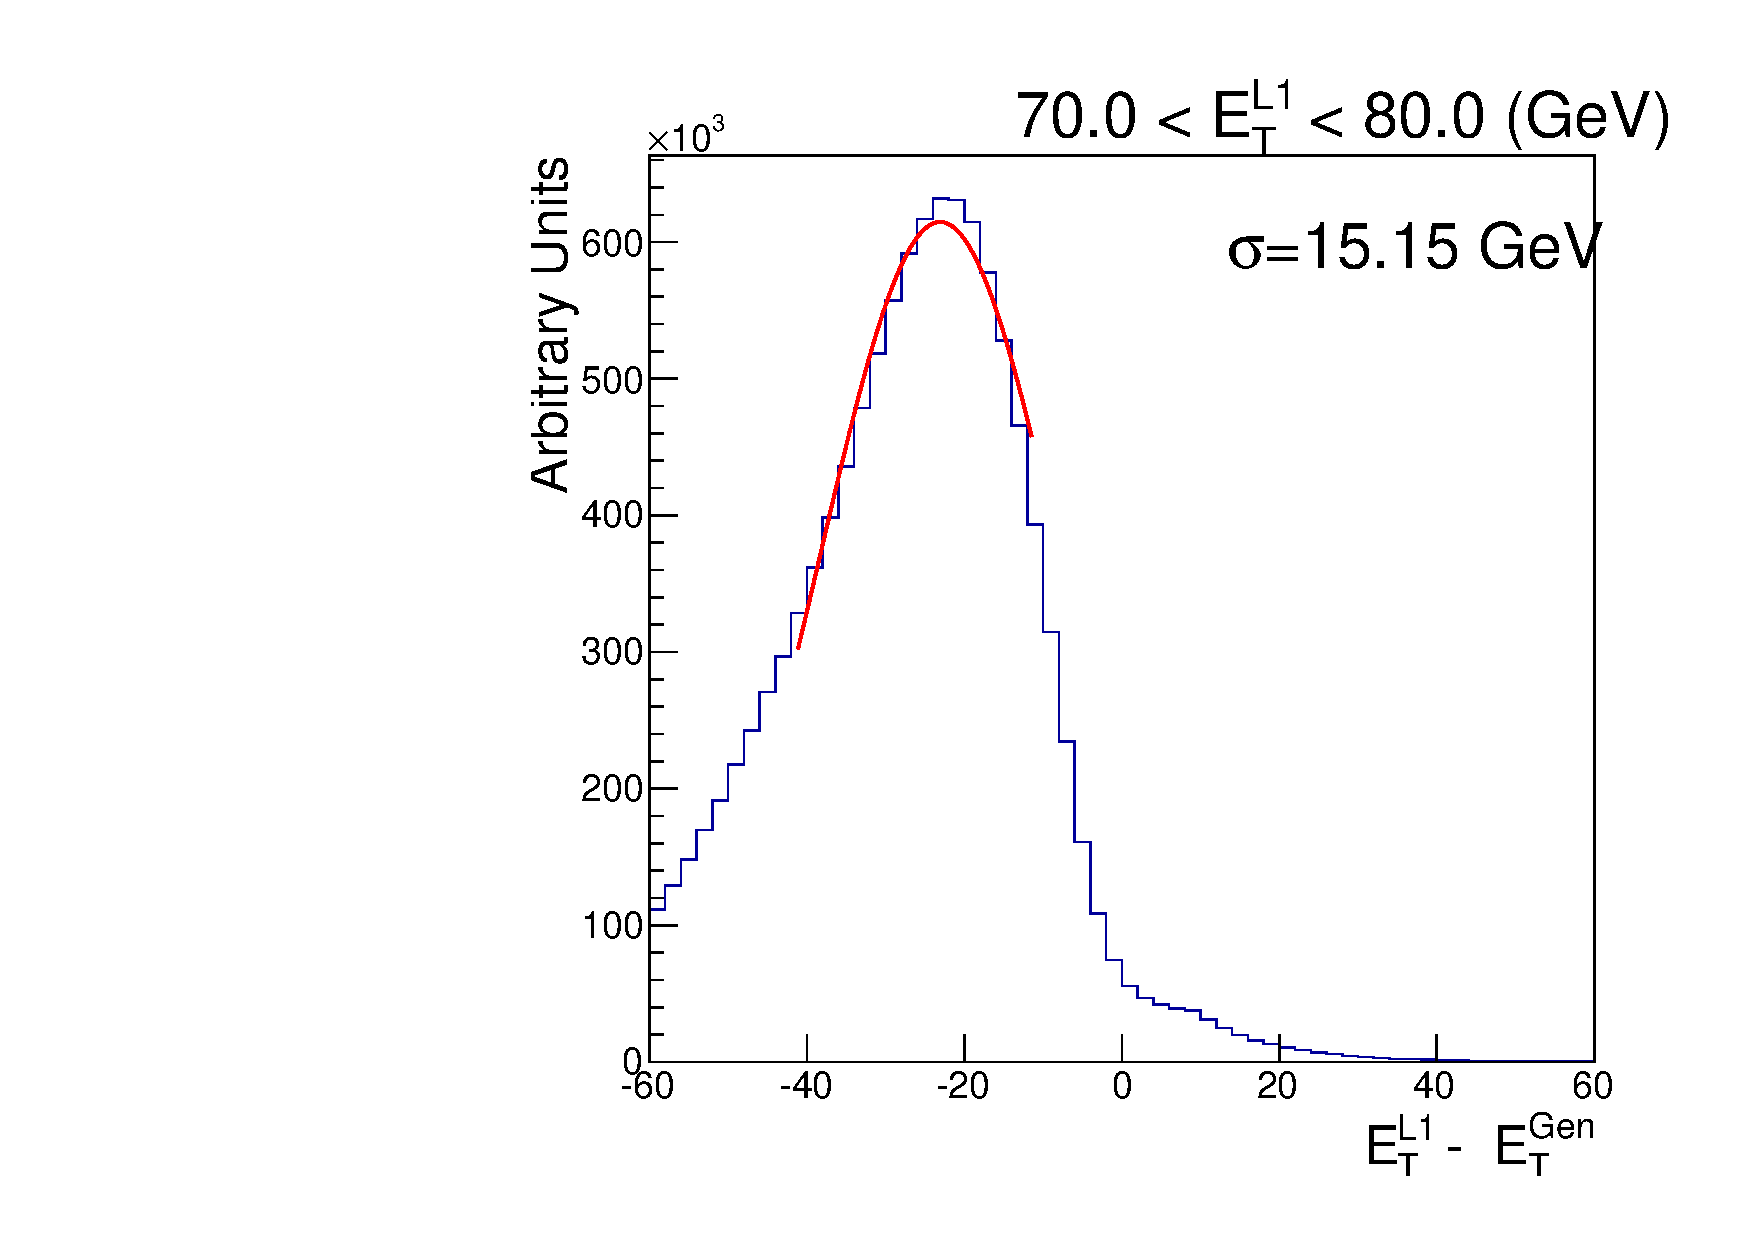
\includegraphics[width=0.32\textwidth]{detector/l1jet/gaussfits//ptBin_9_PtAll_u.pdf}\\
          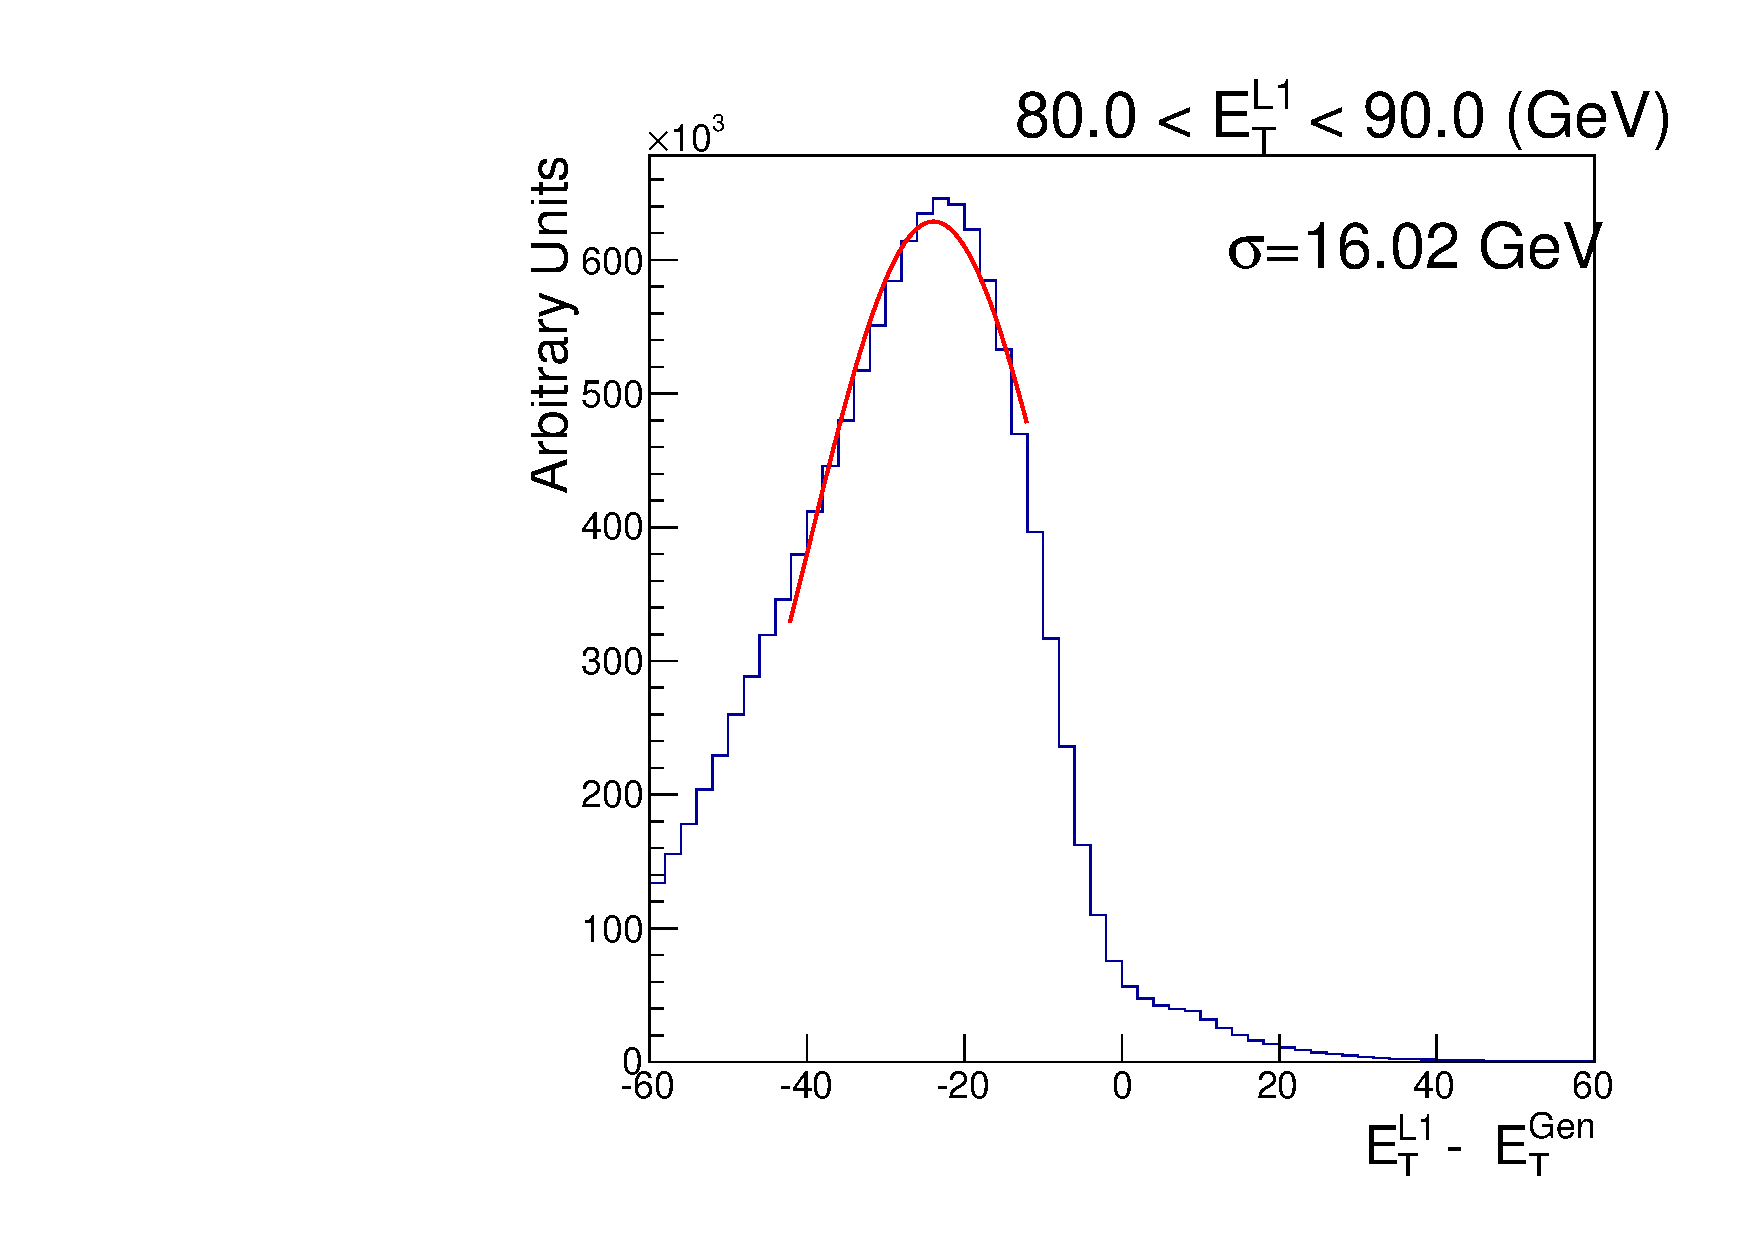
\includegraphics[width=0.32\textwidth]{detector/l1jet/gaussfits//ptBin_10_PtAll_u.pdf}
          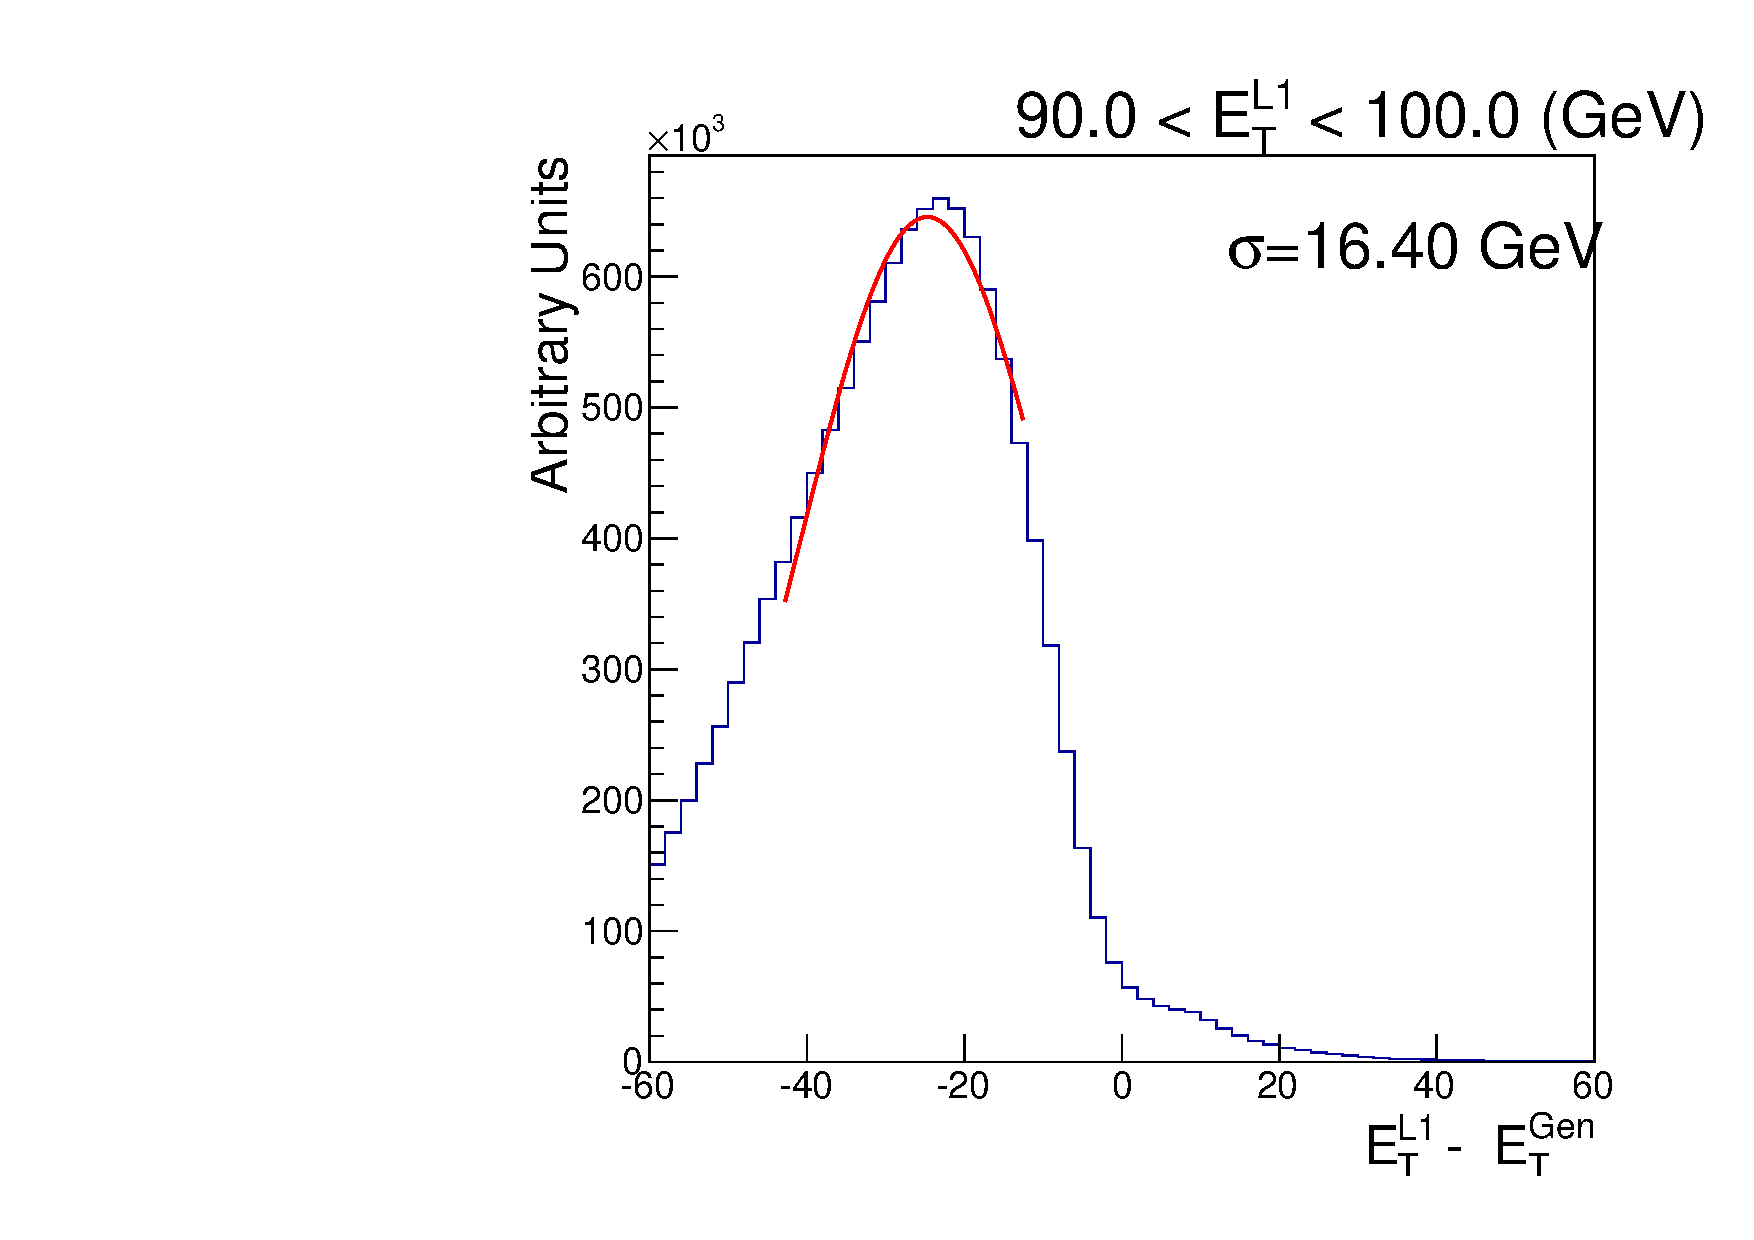
\includegraphics[width=0.32\textwidth]{detector/l1jet/gaussfits//ptBin_11_PtAll_u.pdf}
          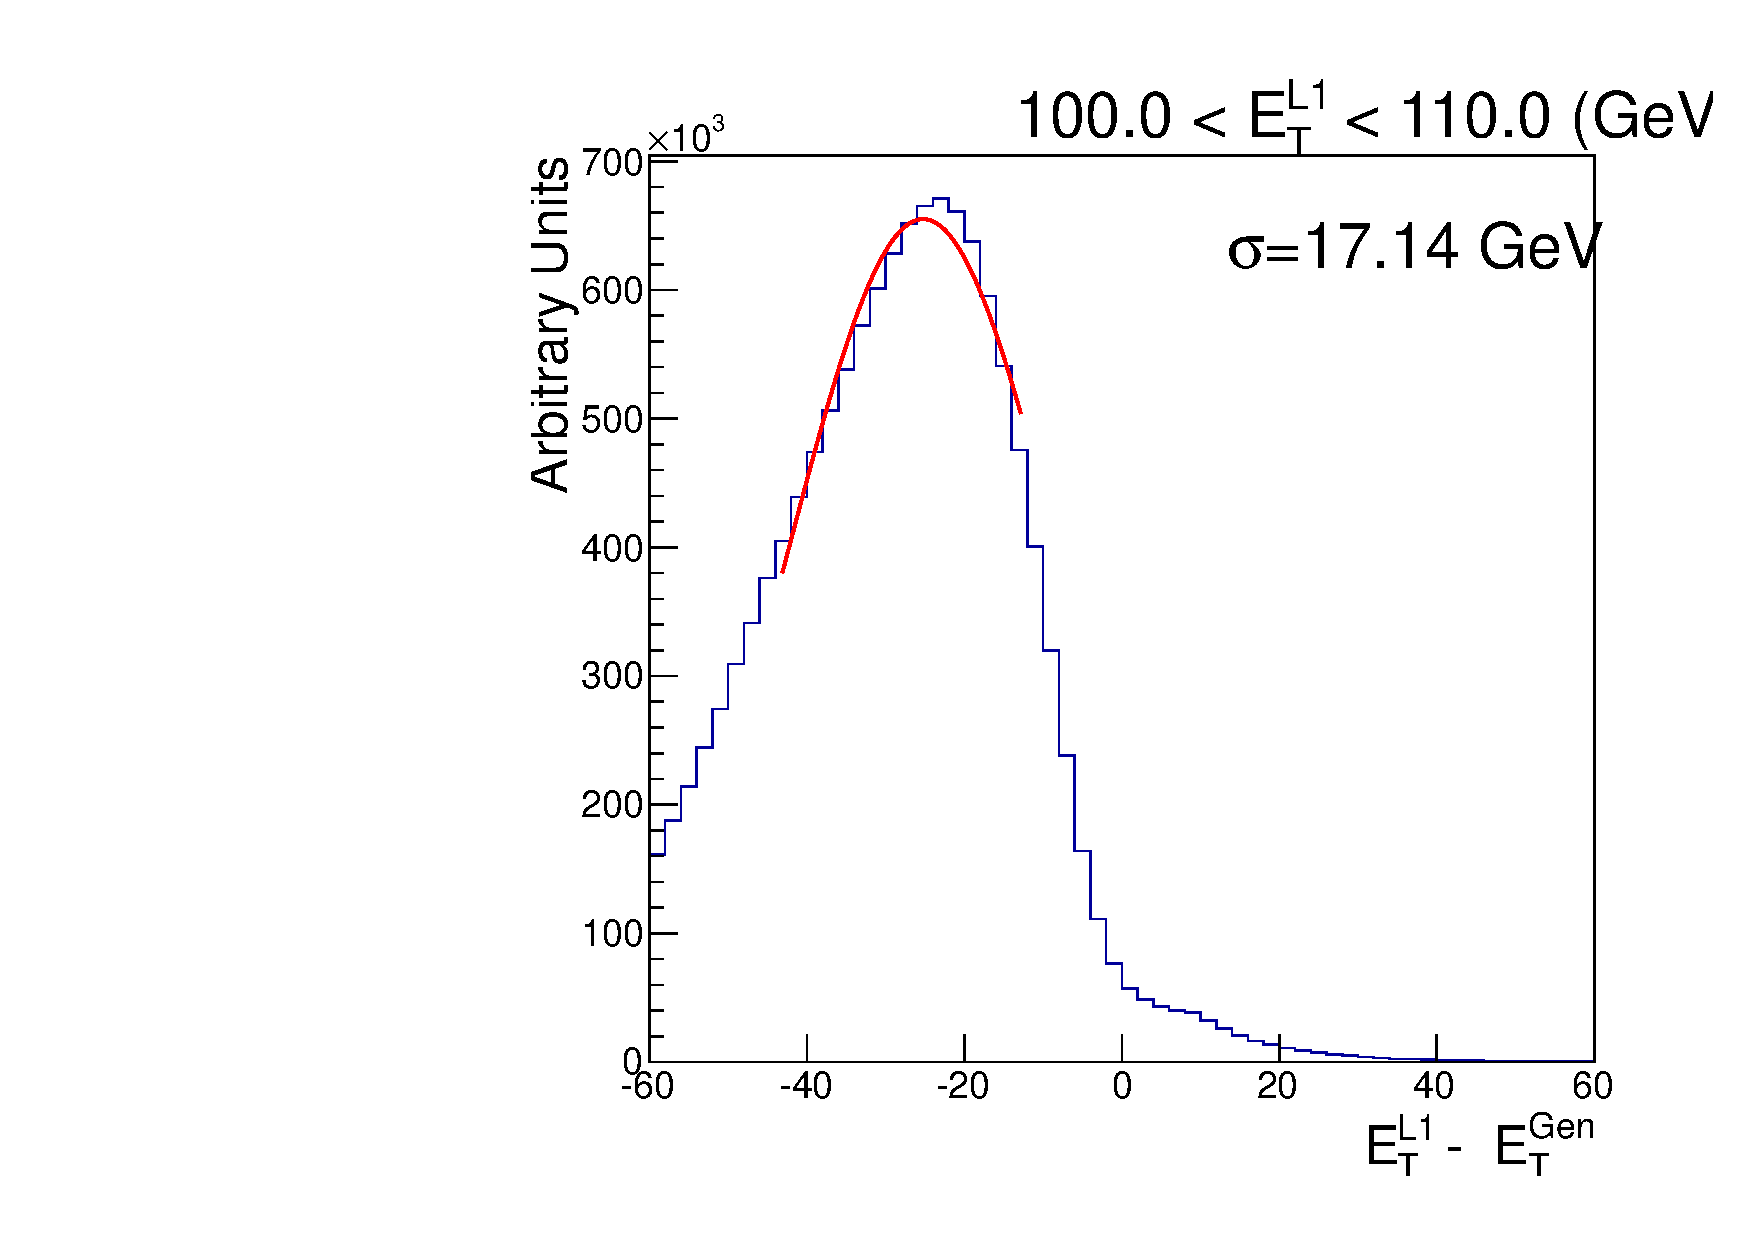
\includegraphics[width=0.32\textwidth]{detector/l1jet/gaussfits//ptBin_12_PtAll_u.pdf}
    \caption{Part two of the distributions of $\Lonept-\Genpt$ in bins of $\Lonept$ of the uncorrected MC jets. 
	The fitted Gaussian is used to extract the resolution as a function of $\Lonept$.}
    \label{fig:mcresfits_u_p2}
\end{figure}
\begin{figure}[h!]
    \centering
          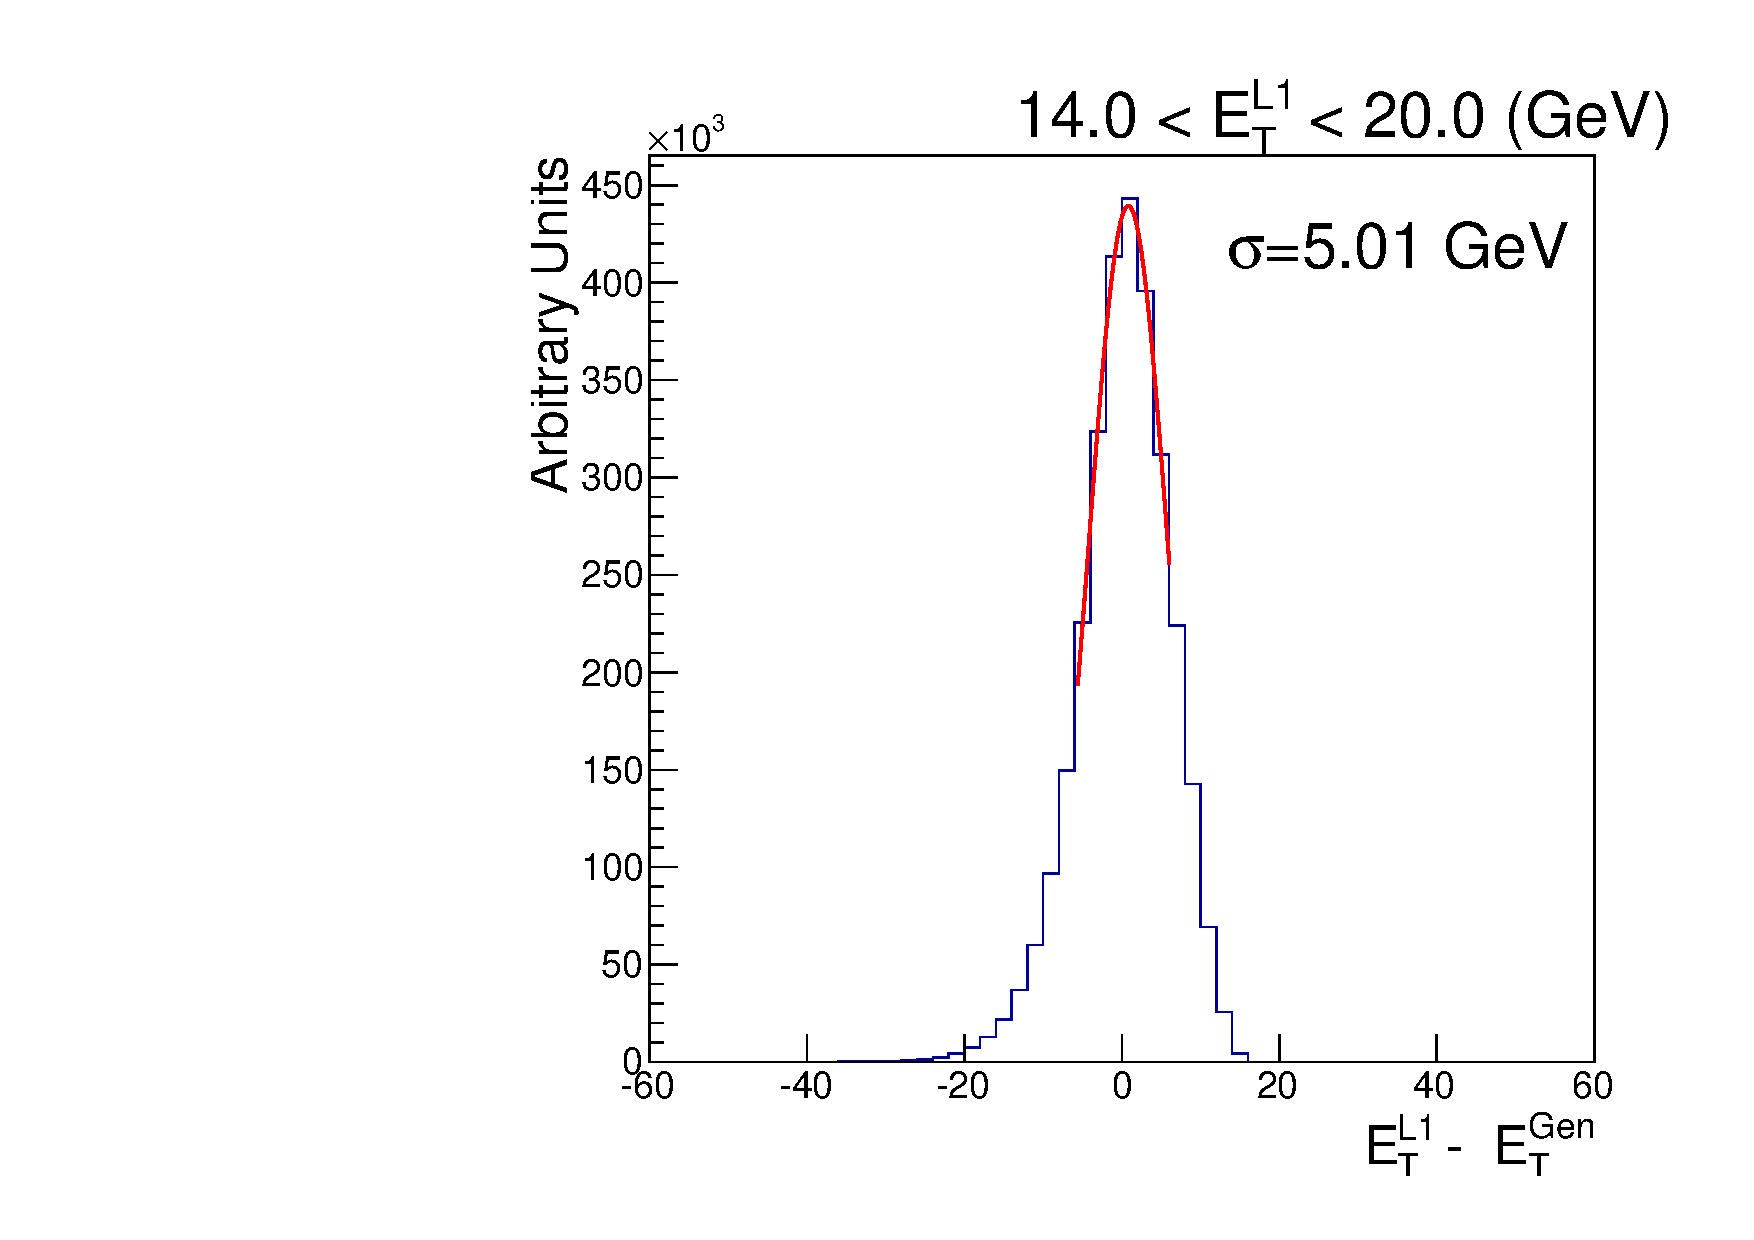
\includegraphics[width=0.32\textwidth]{detector/l1jet/gaussfits//ptBin_0_PtAll_pf.pdf}
          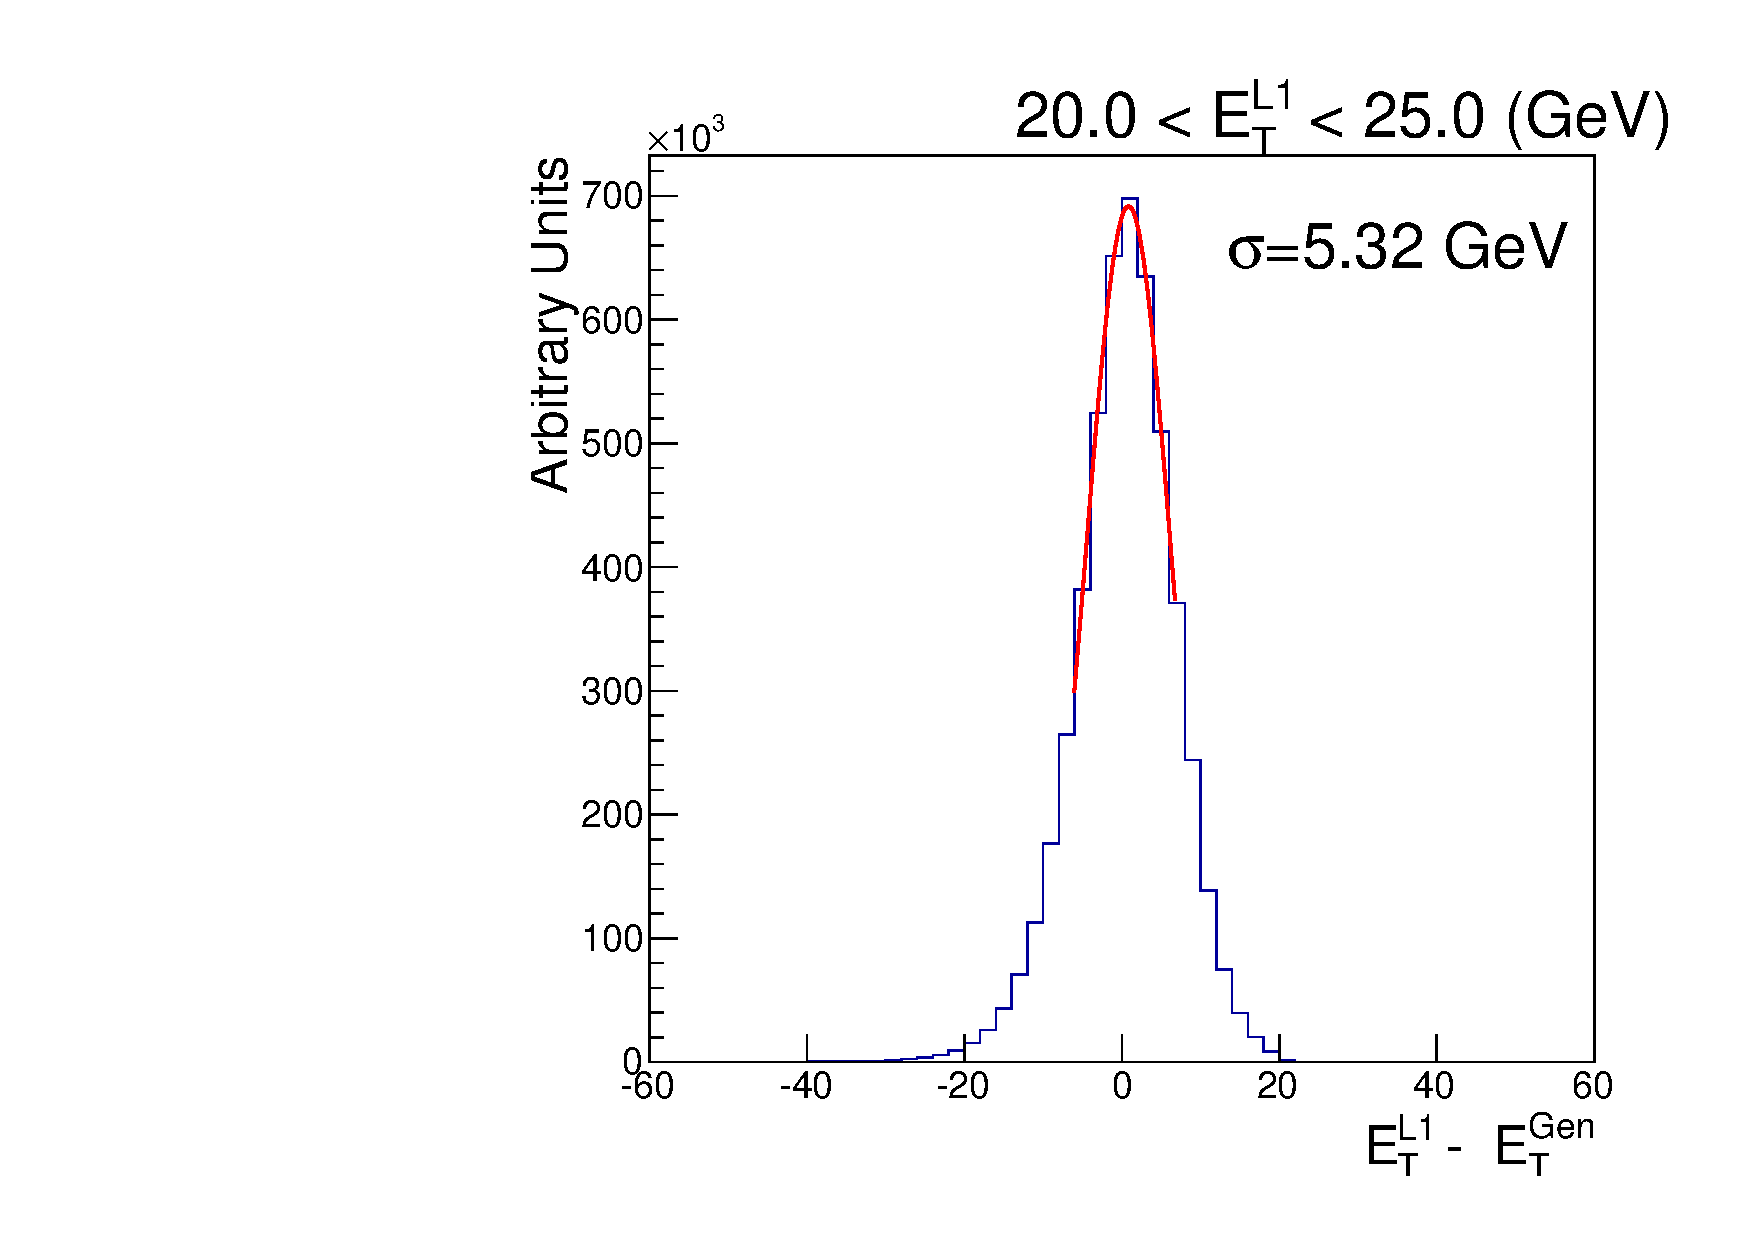
\includegraphics[width=0.32\textwidth]{detector/l1jet/gaussfits//ptBin_1_PtAll_pf.pdf}
          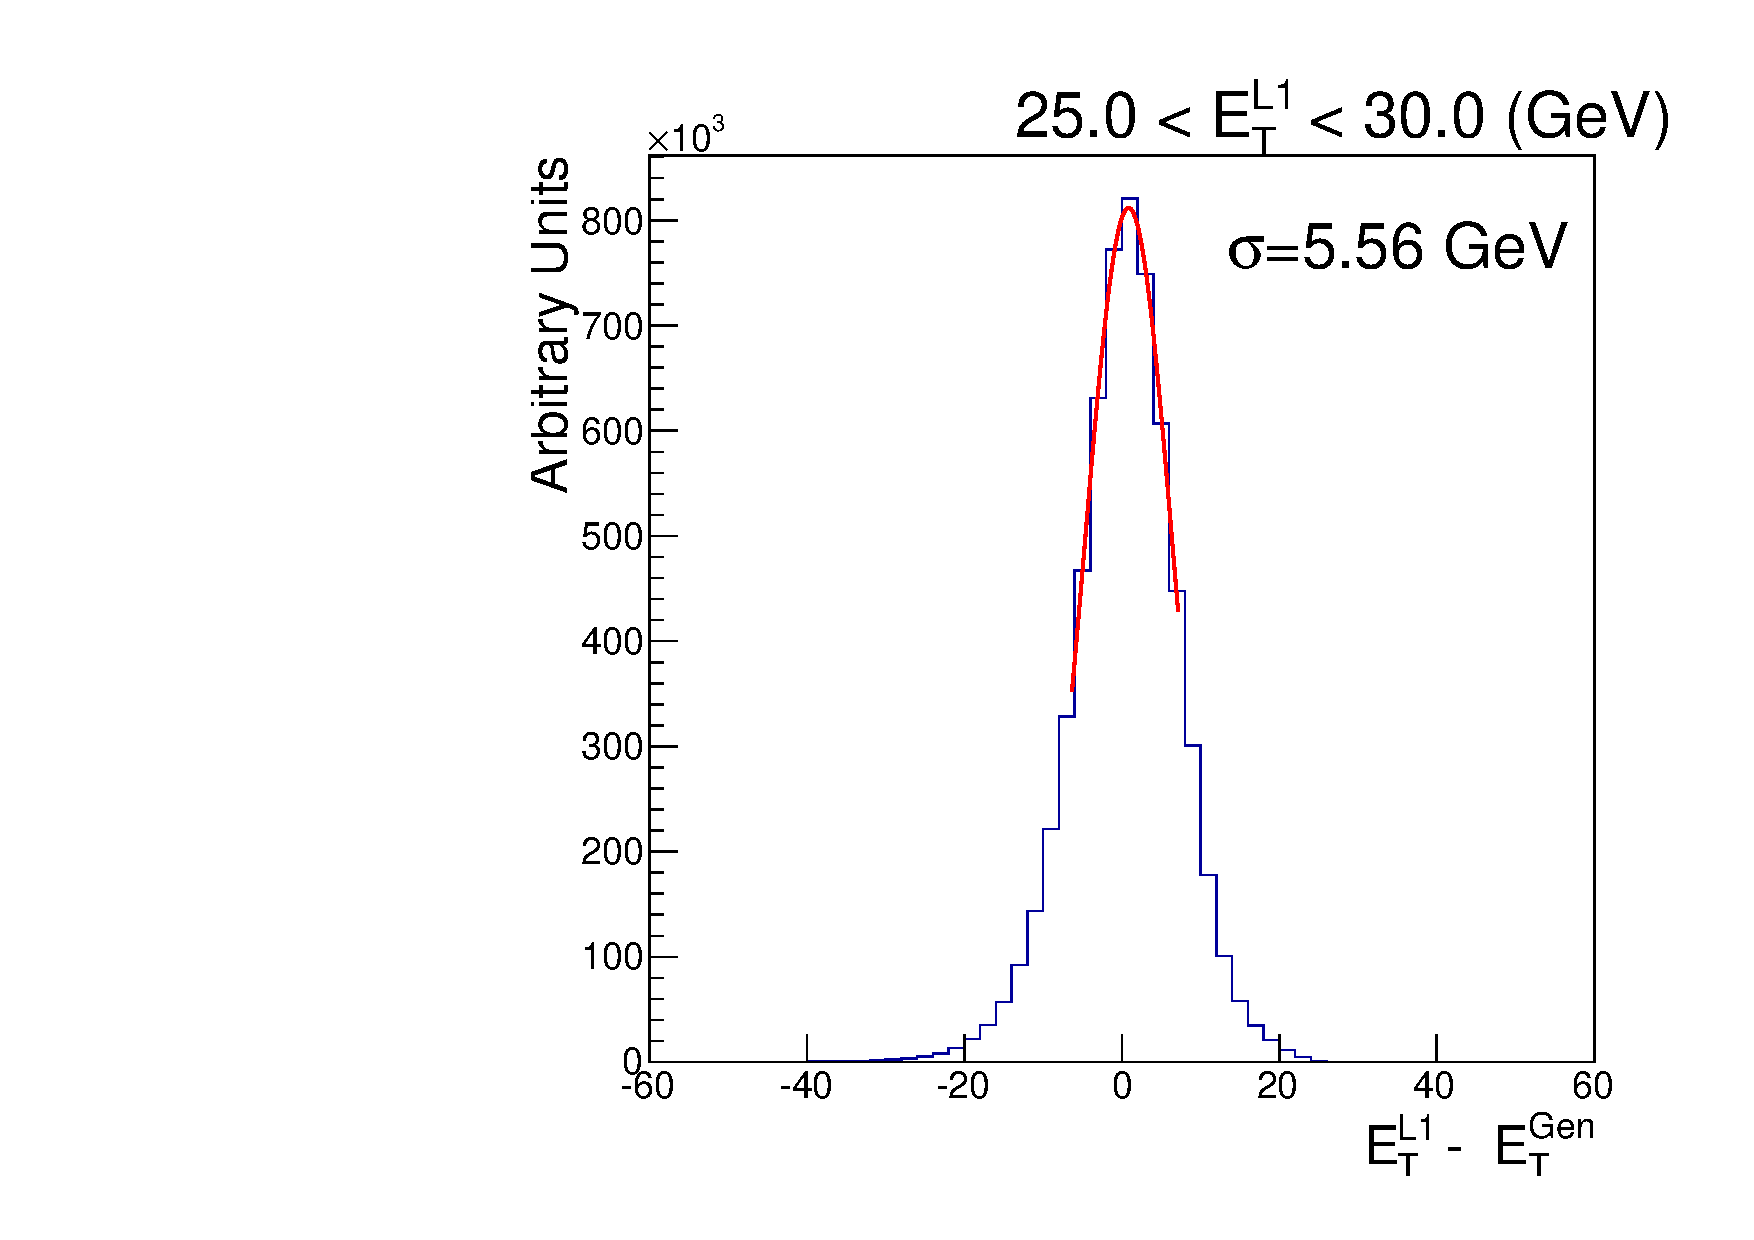
\includegraphics[width=0.32\textwidth]{detector/l1jet/gaussfits//ptBin_2_PtAll_pf.pdf}\\
          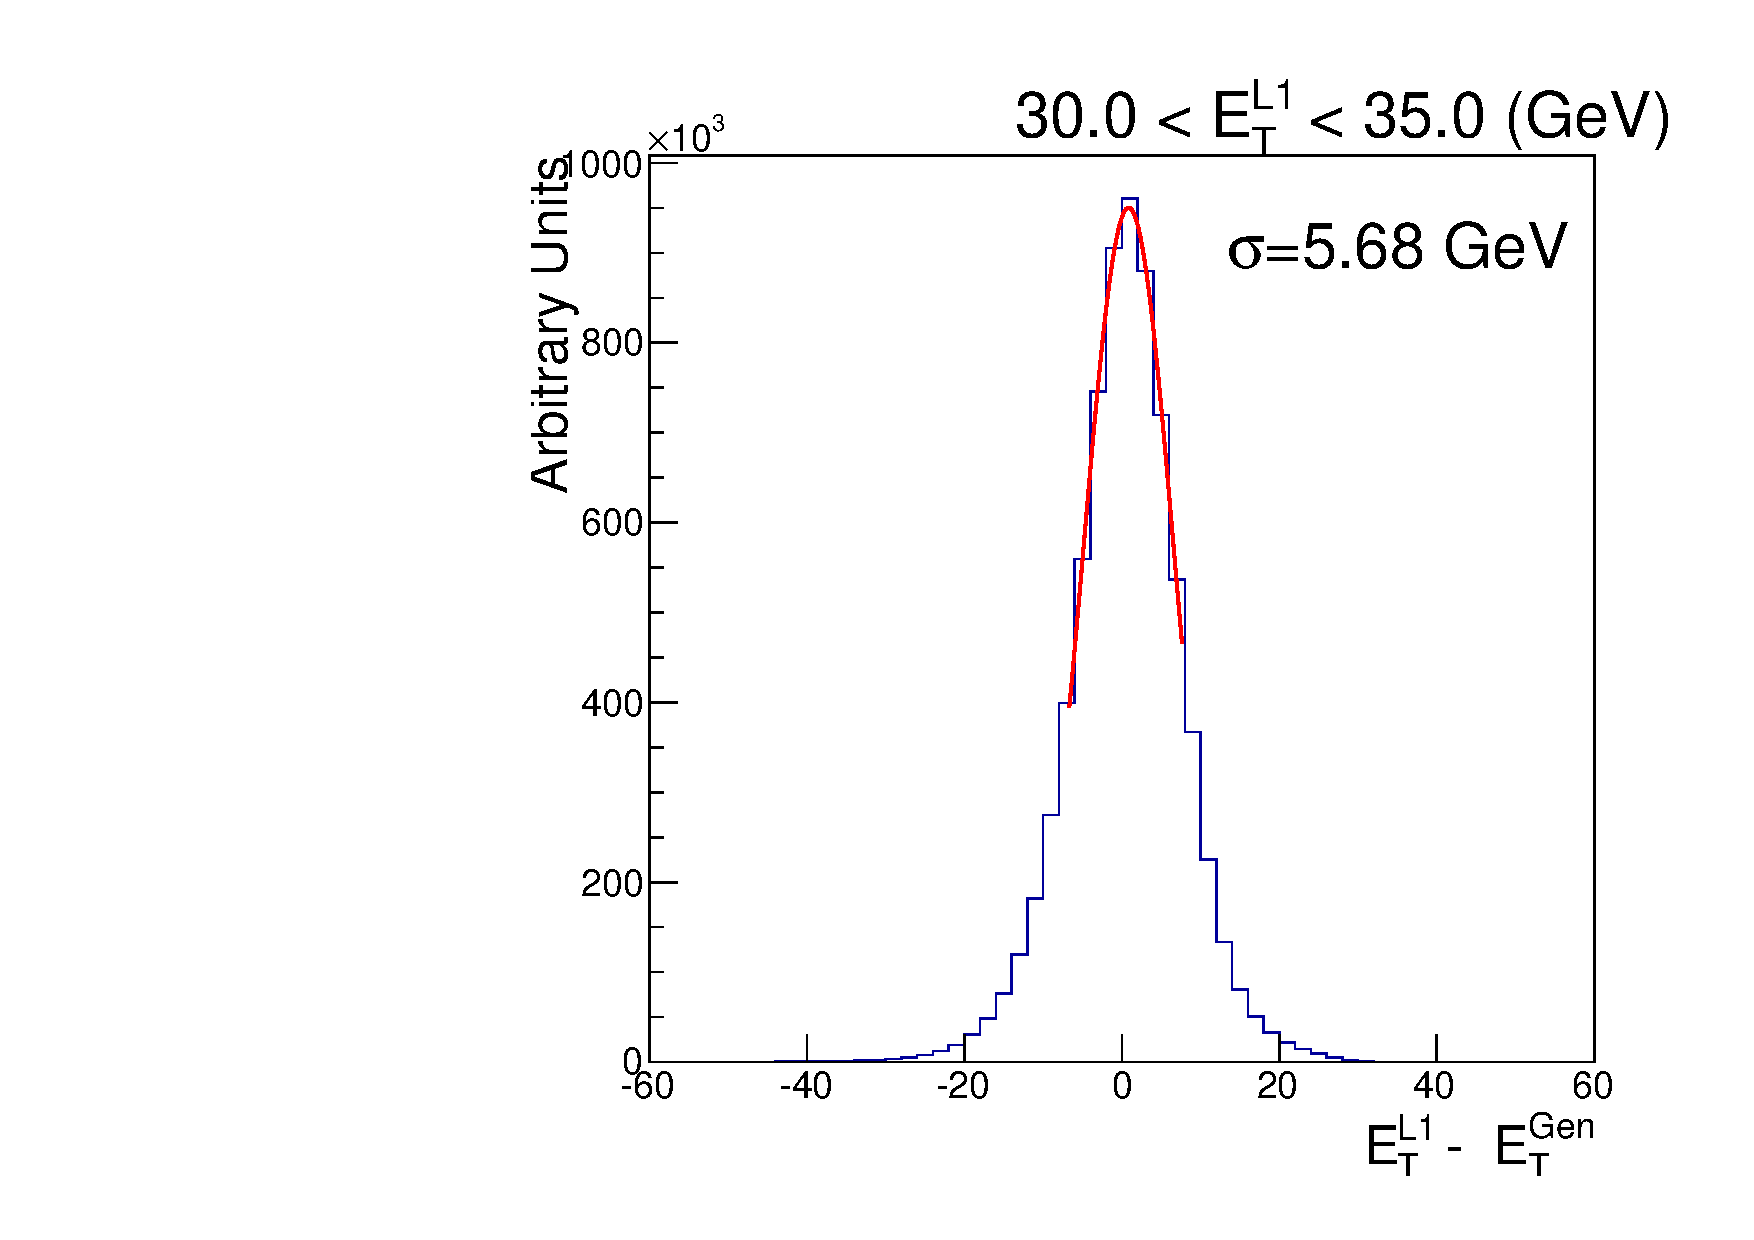
\includegraphics[width=0.32\textwidth]{detector/l1jet/gaussfits//ptBin_3_PtAll_pf.pdf}
          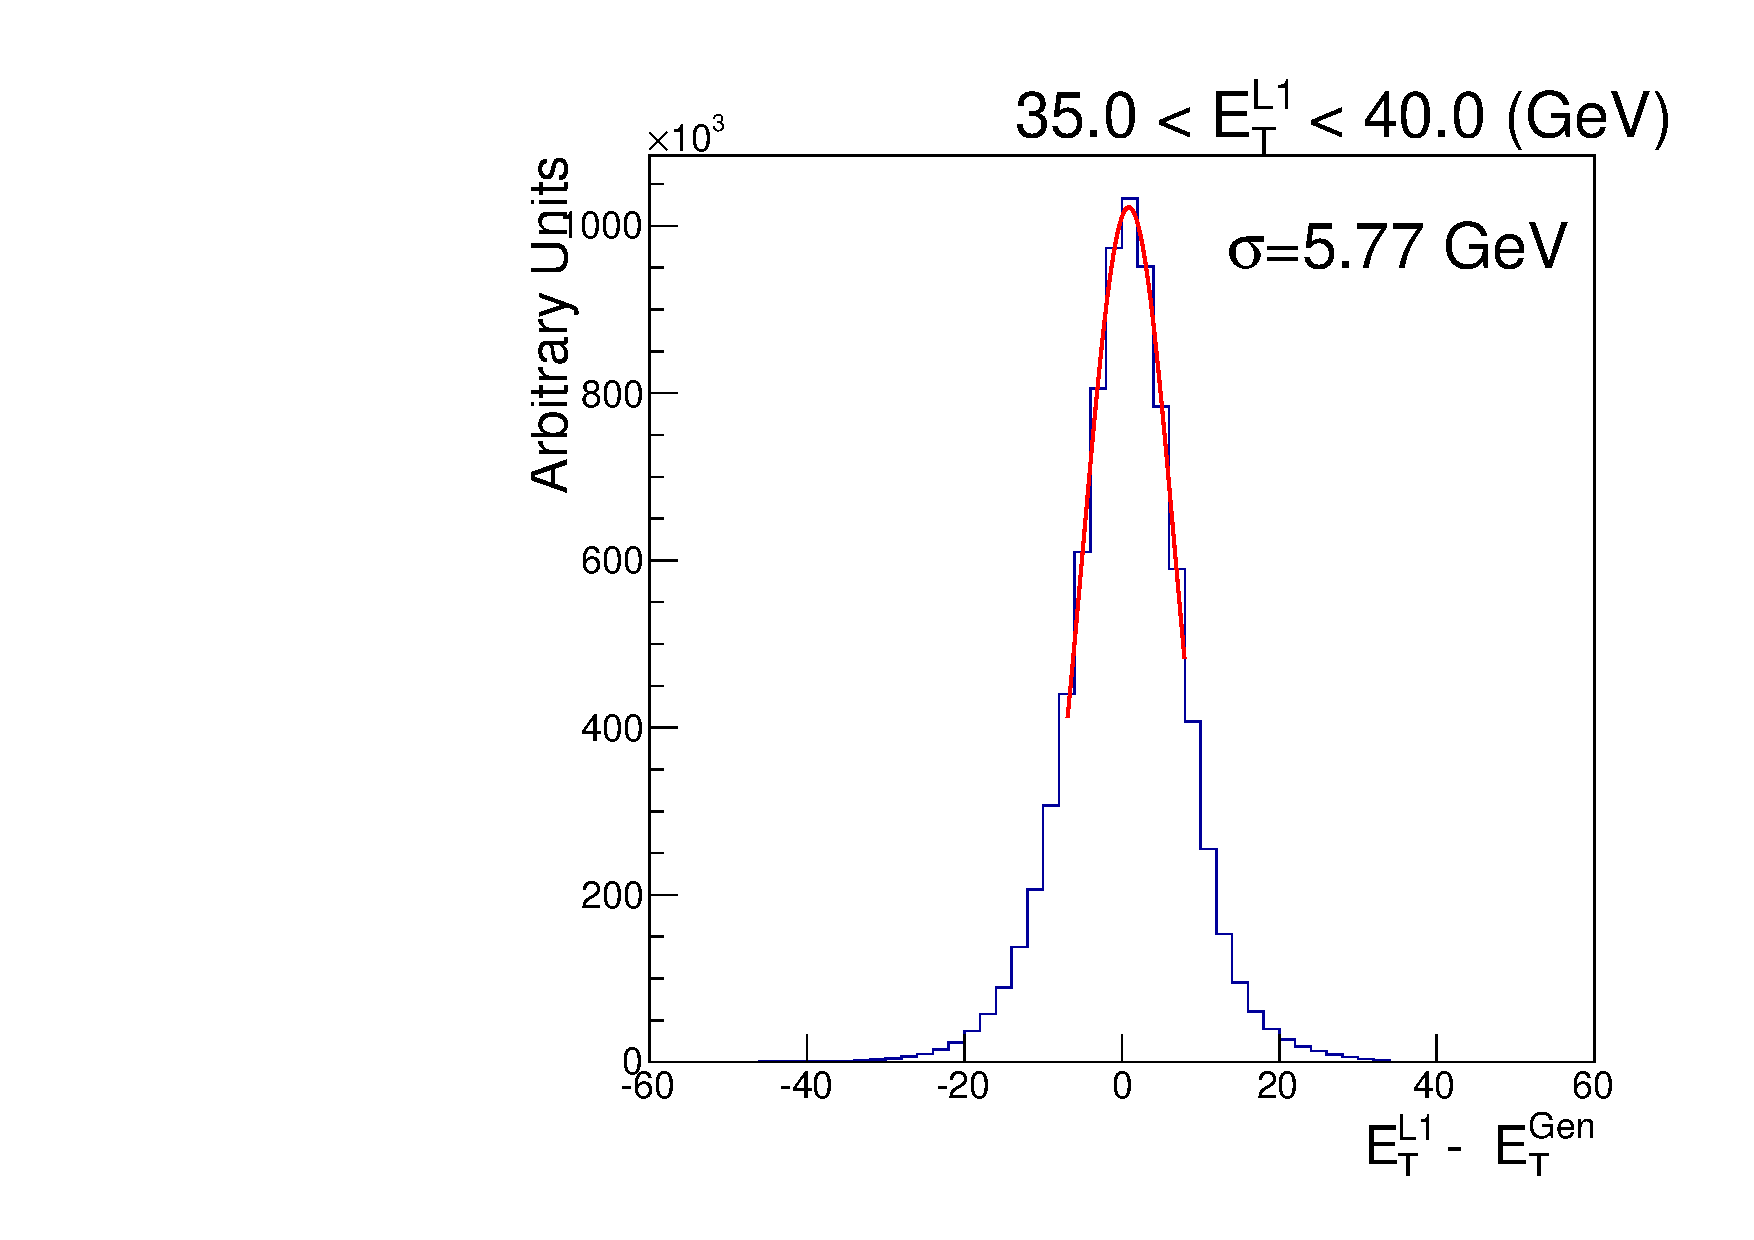
\includegraphics[width=0.32\textwidth]{detector/l1jet/gaussfits//ptBin_4_PtAll_pf.pdf}
          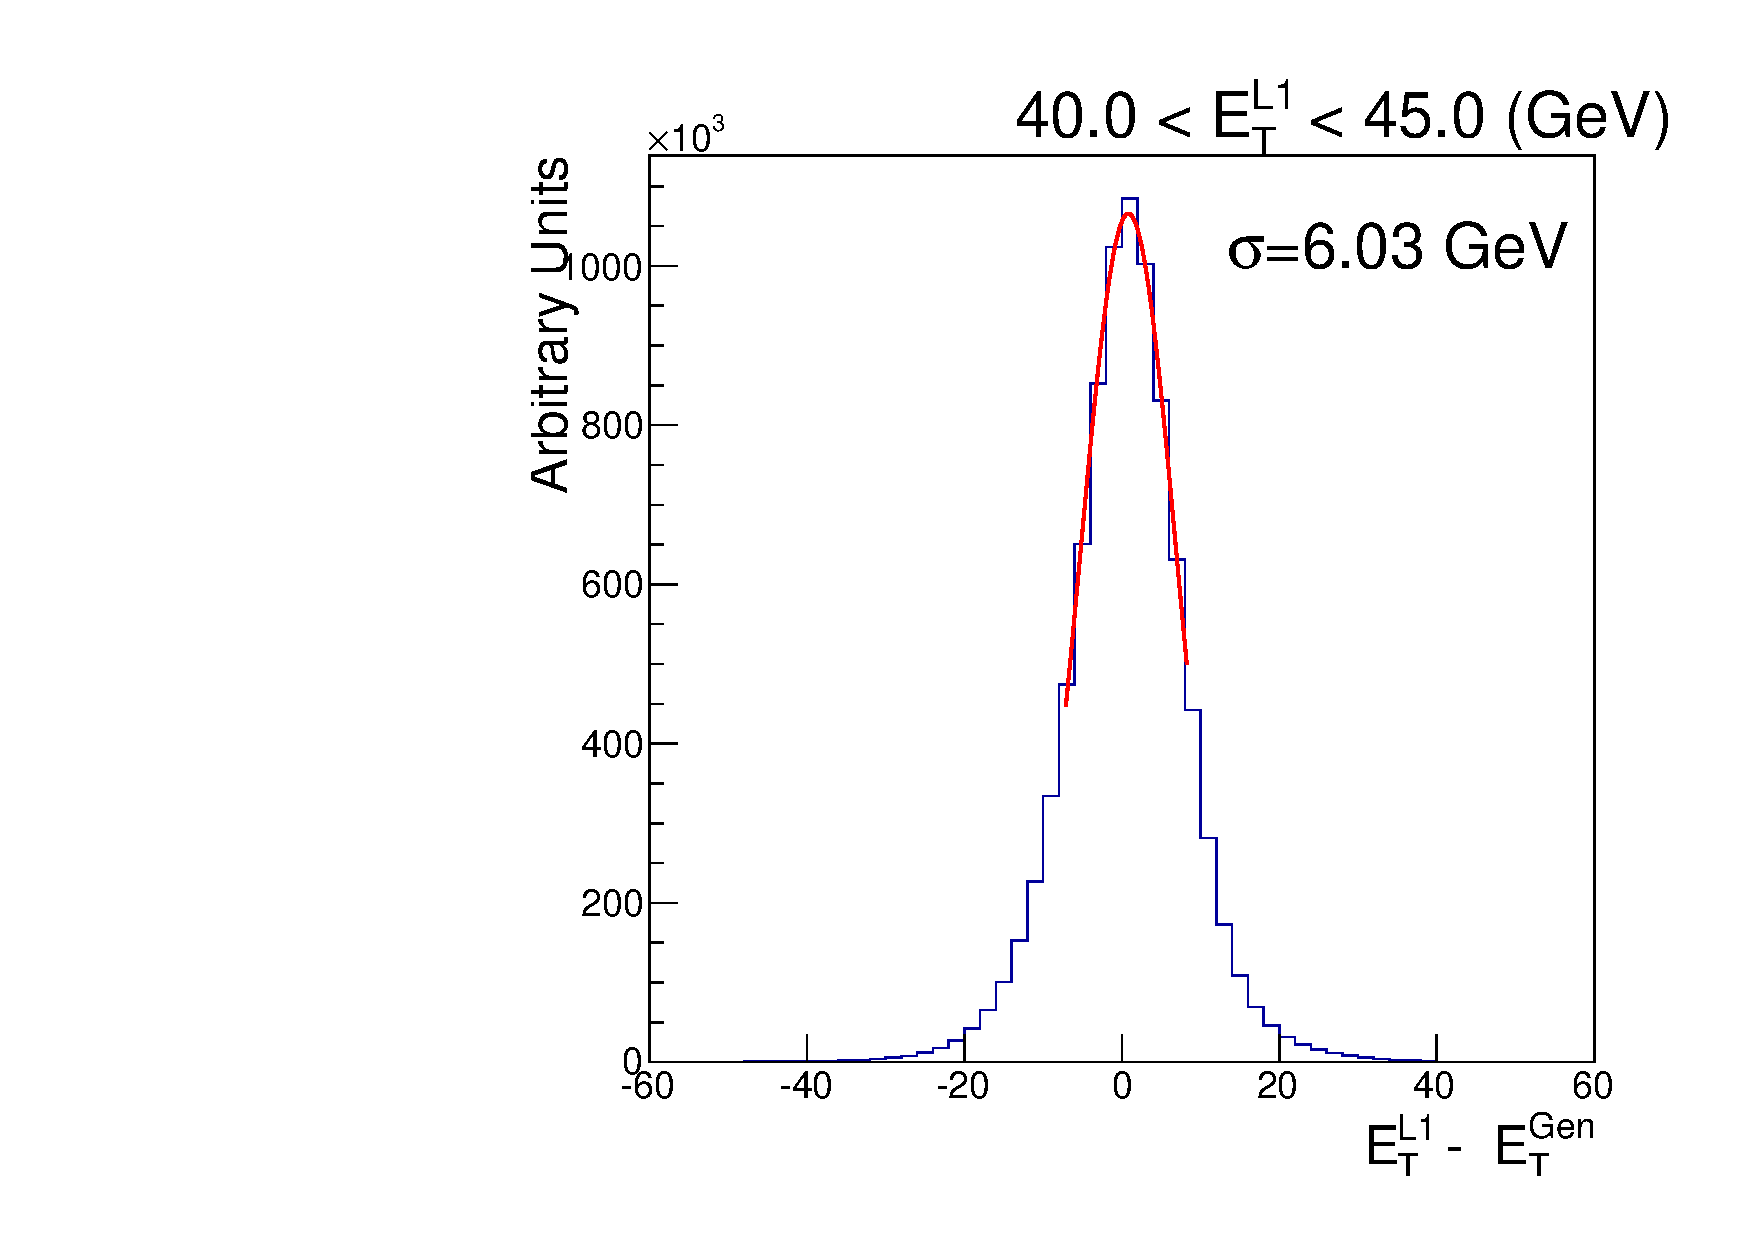
\includegraphics[width=0.32\textwidth]{detector/l1jet/gaussfits//ptBin_5_PtAll_pf.pdf}\\
          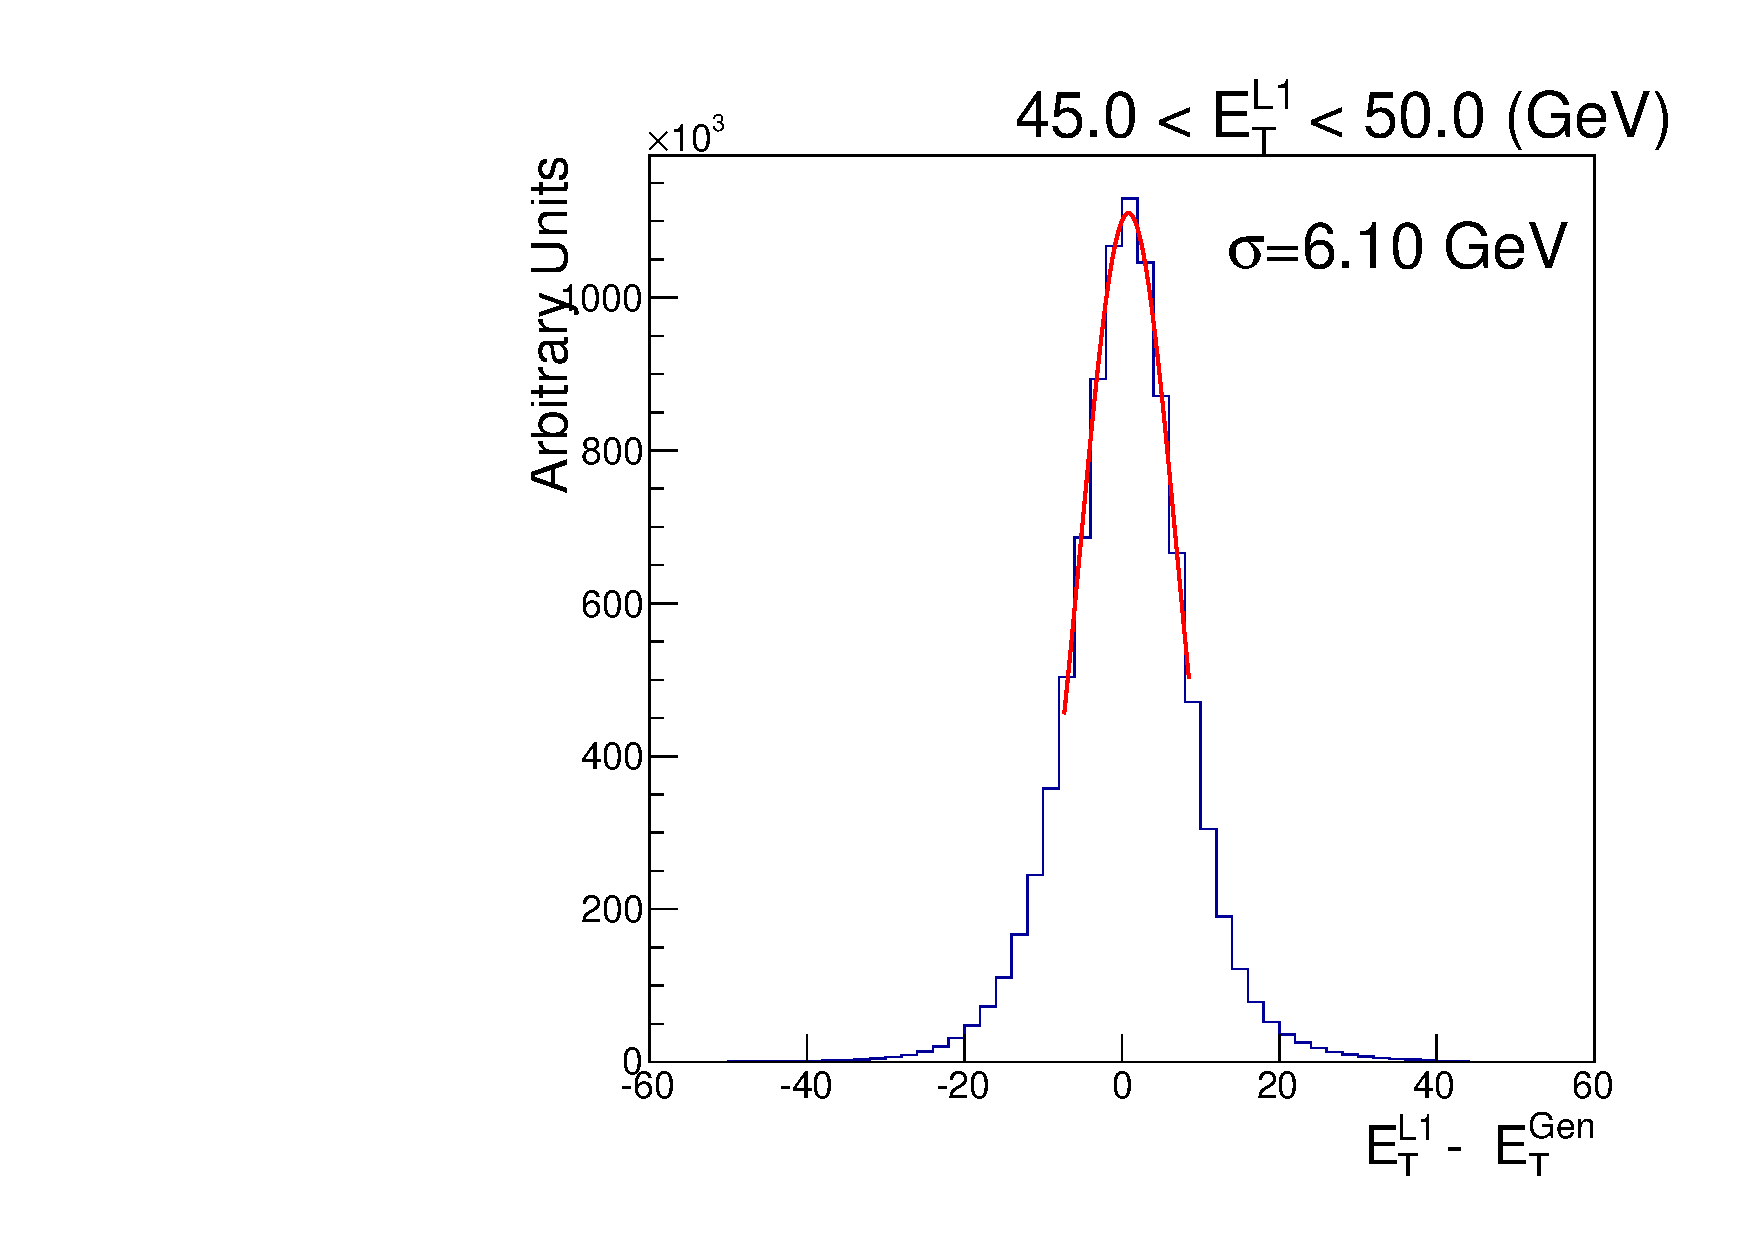
\includegraphics[width=0.32\textwidth]{detector/l1jet/gaussfits//ptBin_6_PtAll_pf.pdf}
    \caption{Part one of the distributions of $\Lonept-\Genpt$ in bins of $\Lonept$ of the corrected MC jets. 
	The fitted Gaussian is used to extract the resolution as a function of $\Lonept$.}
    \label{fig:mcresfits_pf_p1}
\end{figure}
 
\begin{figure}[h!]
    \centering
          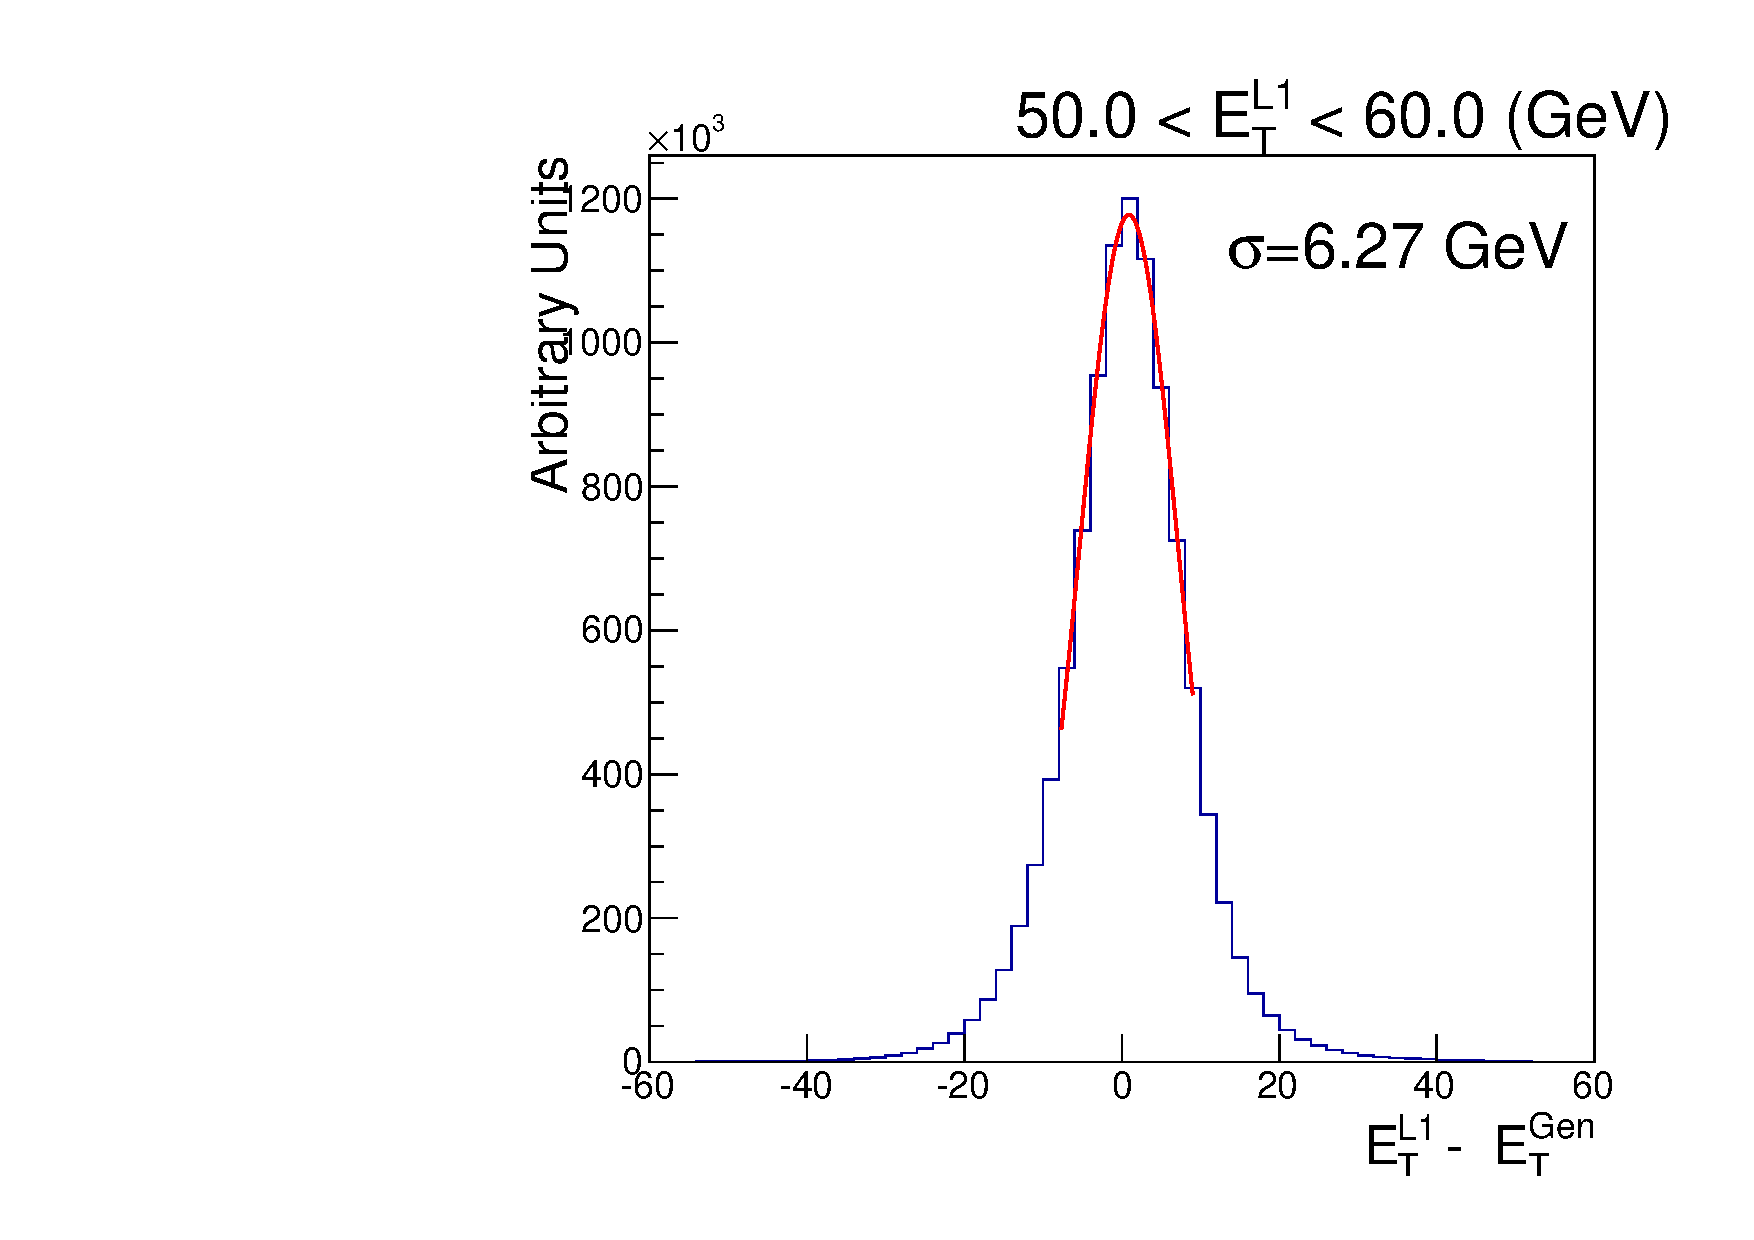
\includegraphics[width=0.32\textwidth]{detector/l1jet/gaussfits//ptBin_7_PtAll_pf.pdf}
          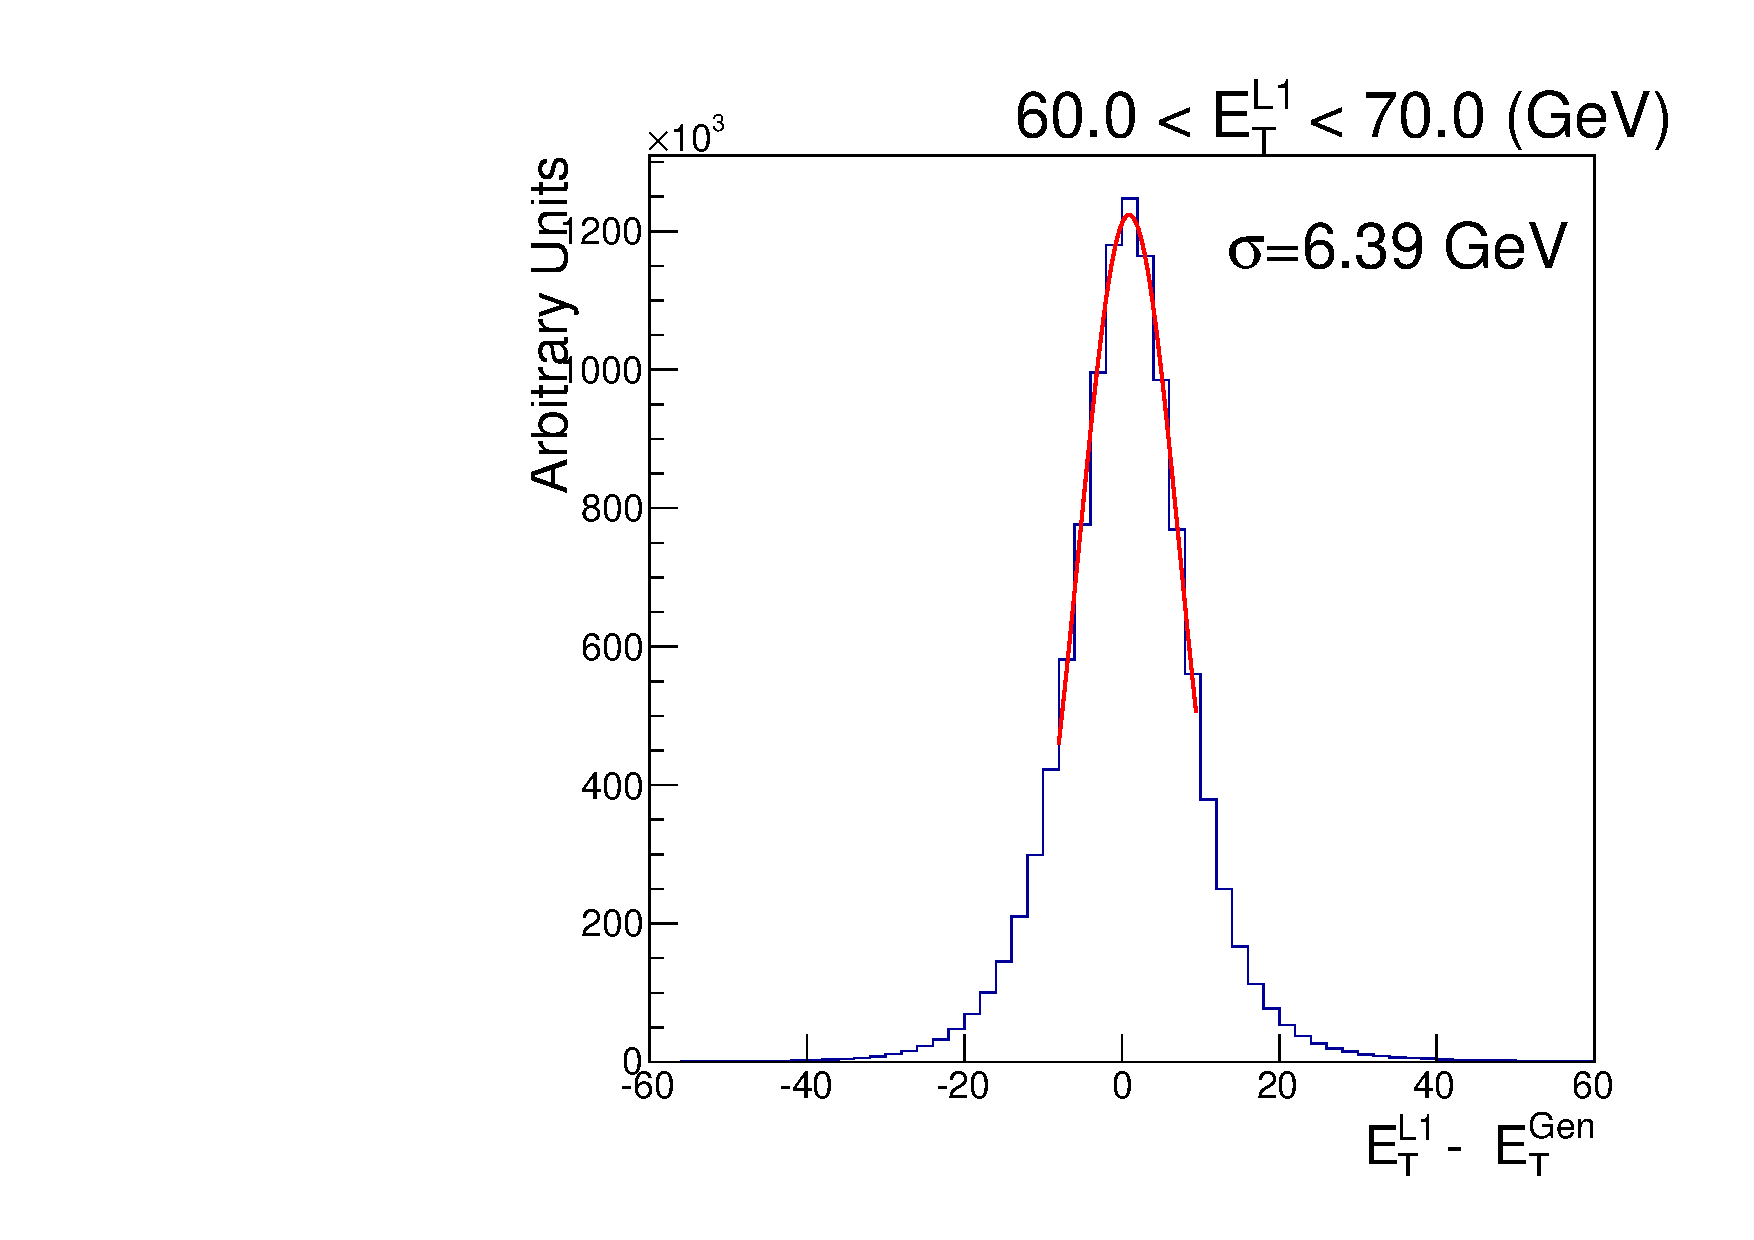
\includegraphics[width=0.32\textwidth]{detector/l1jet/gaussfits//ptBin_8_PtAll_pf.pdf}
          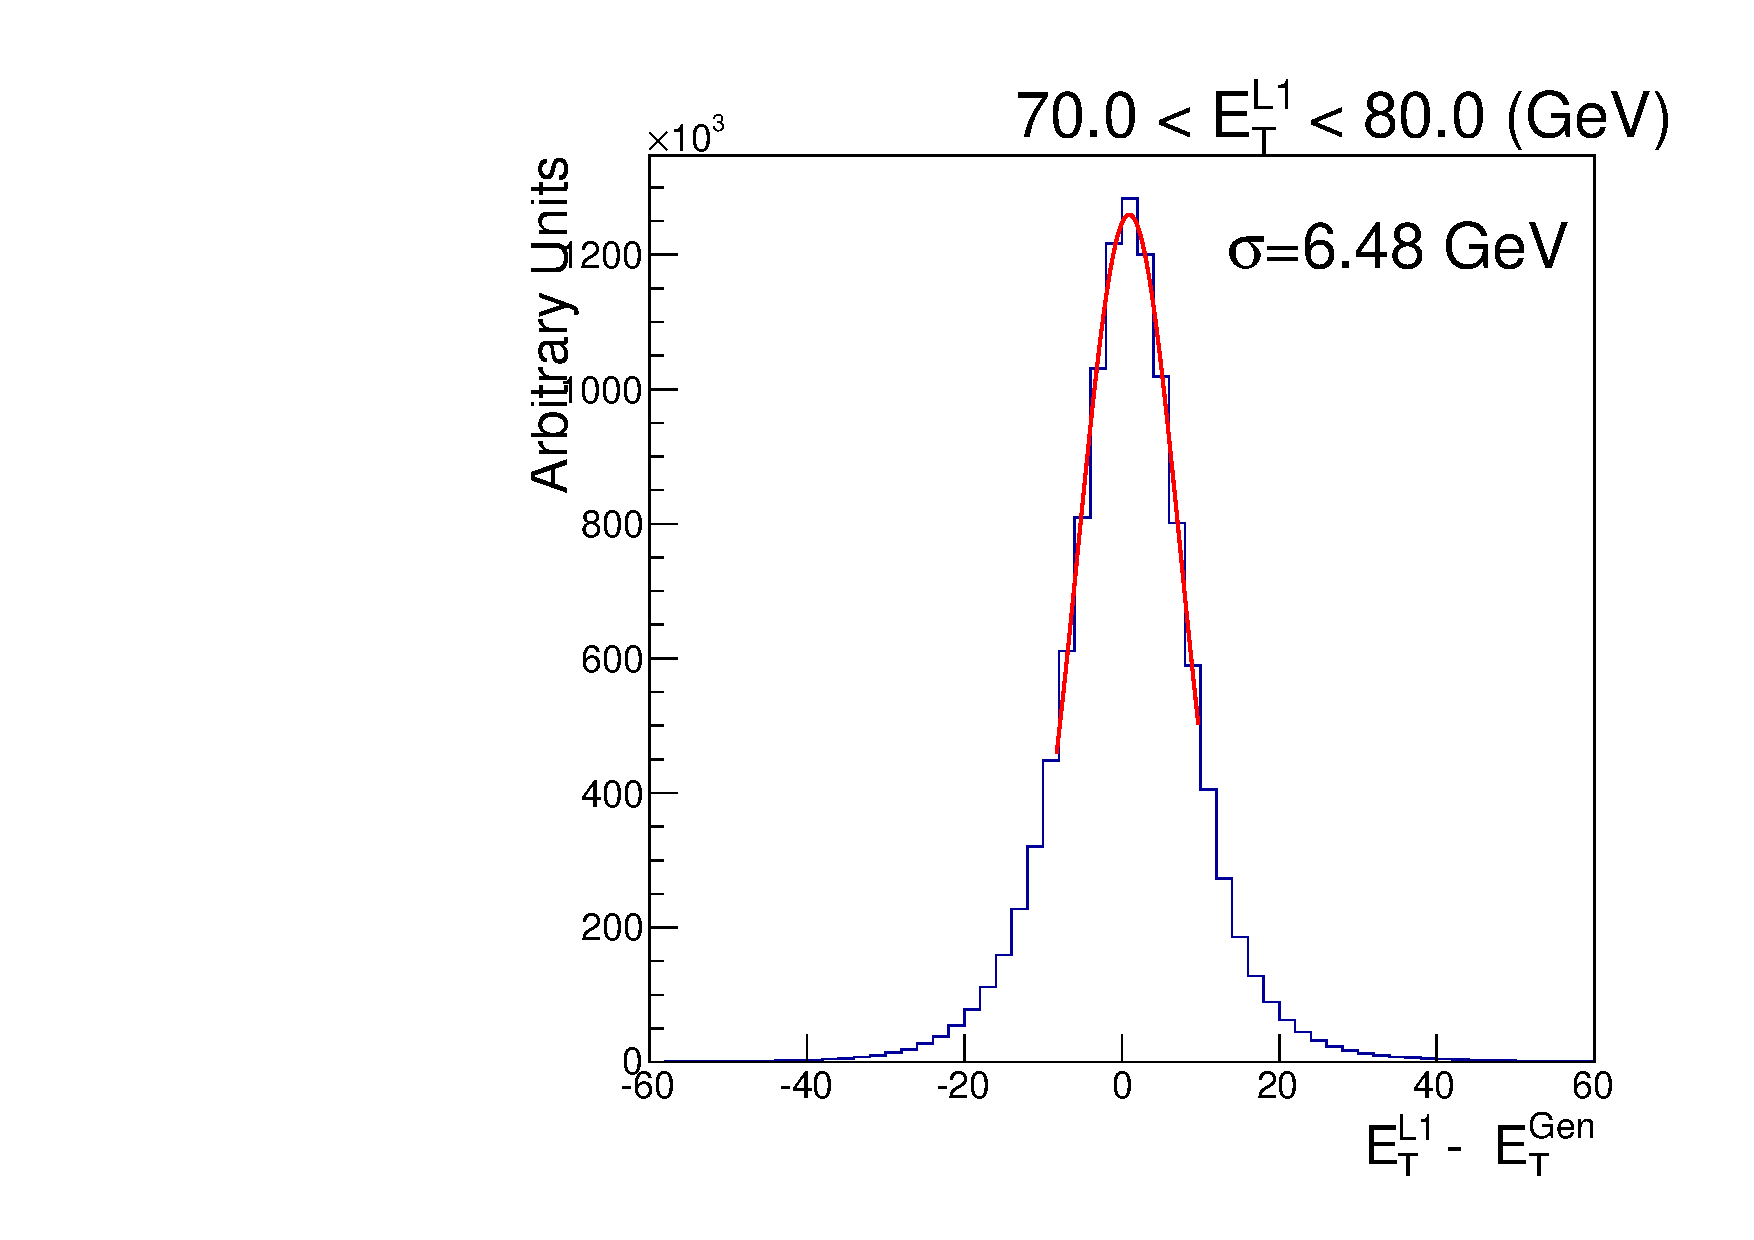
\includegraphics[width=0.32\textwidth]{detector/l1jet/gaussfits//ptBin_9_PtAll_pf.pdf}\\
          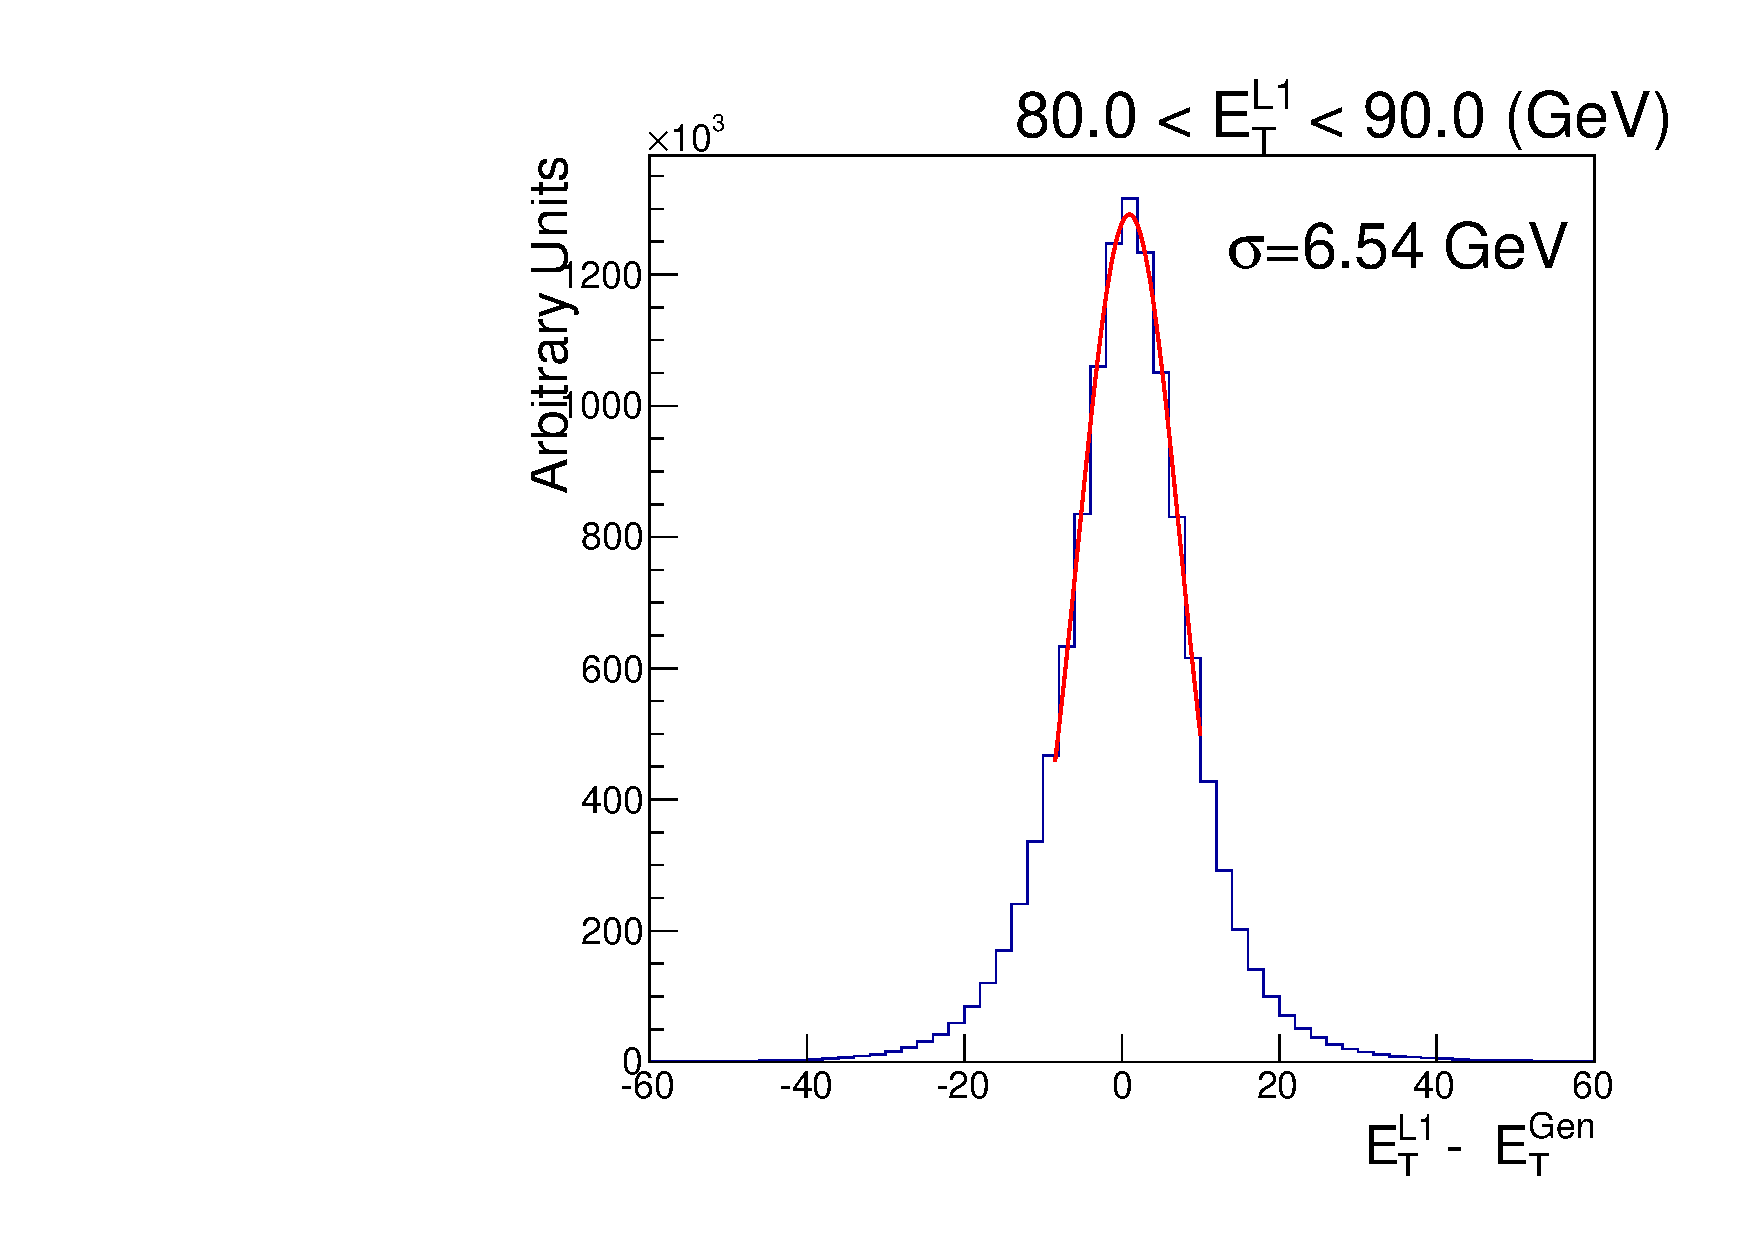
\includegraphics[width=0.32\textwidth]{detector/l1jet/gaussfits//ptBin_10_PtAll_pf.pdf}
          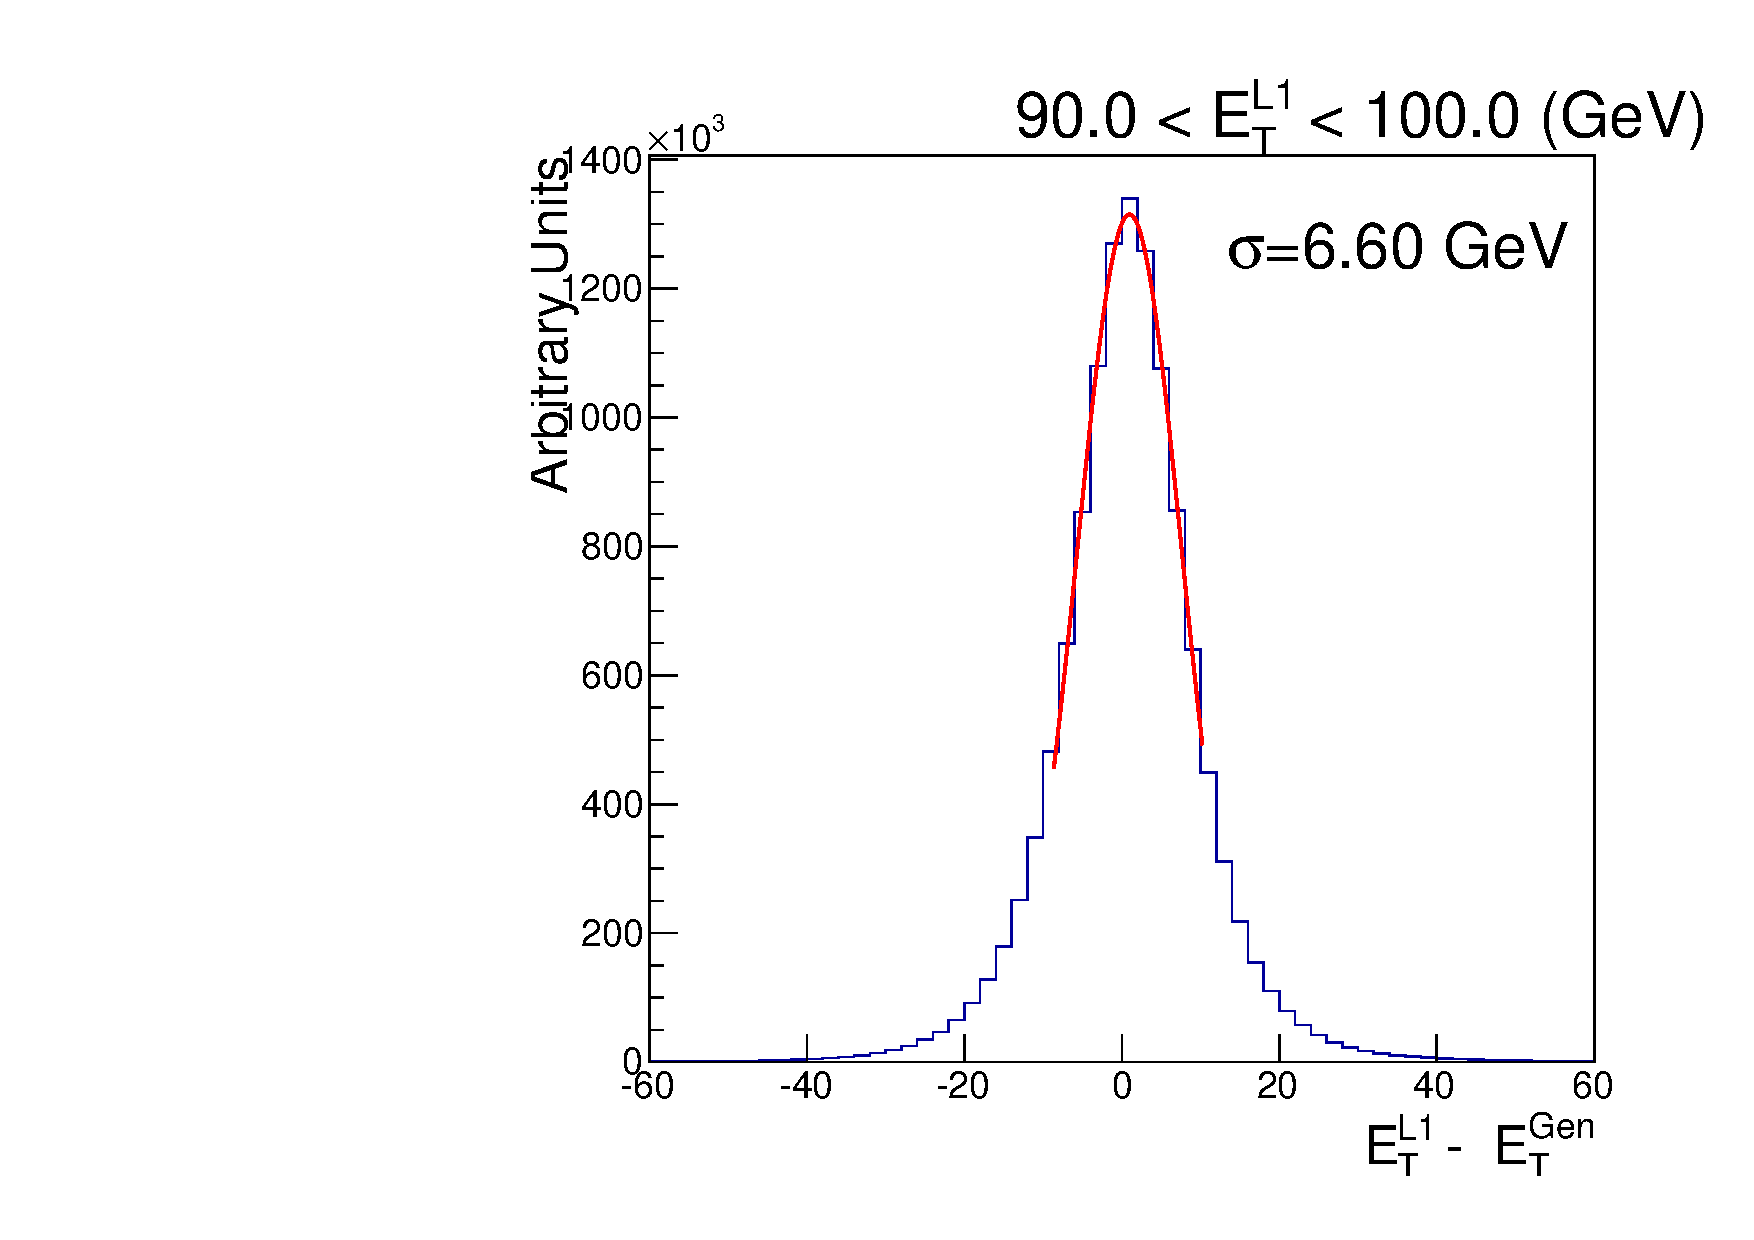
\includegraphics[width=0.32\textwidth]{detector/l1jet/gaussfits//ptBin_11_PtAll_pf.pdf}
          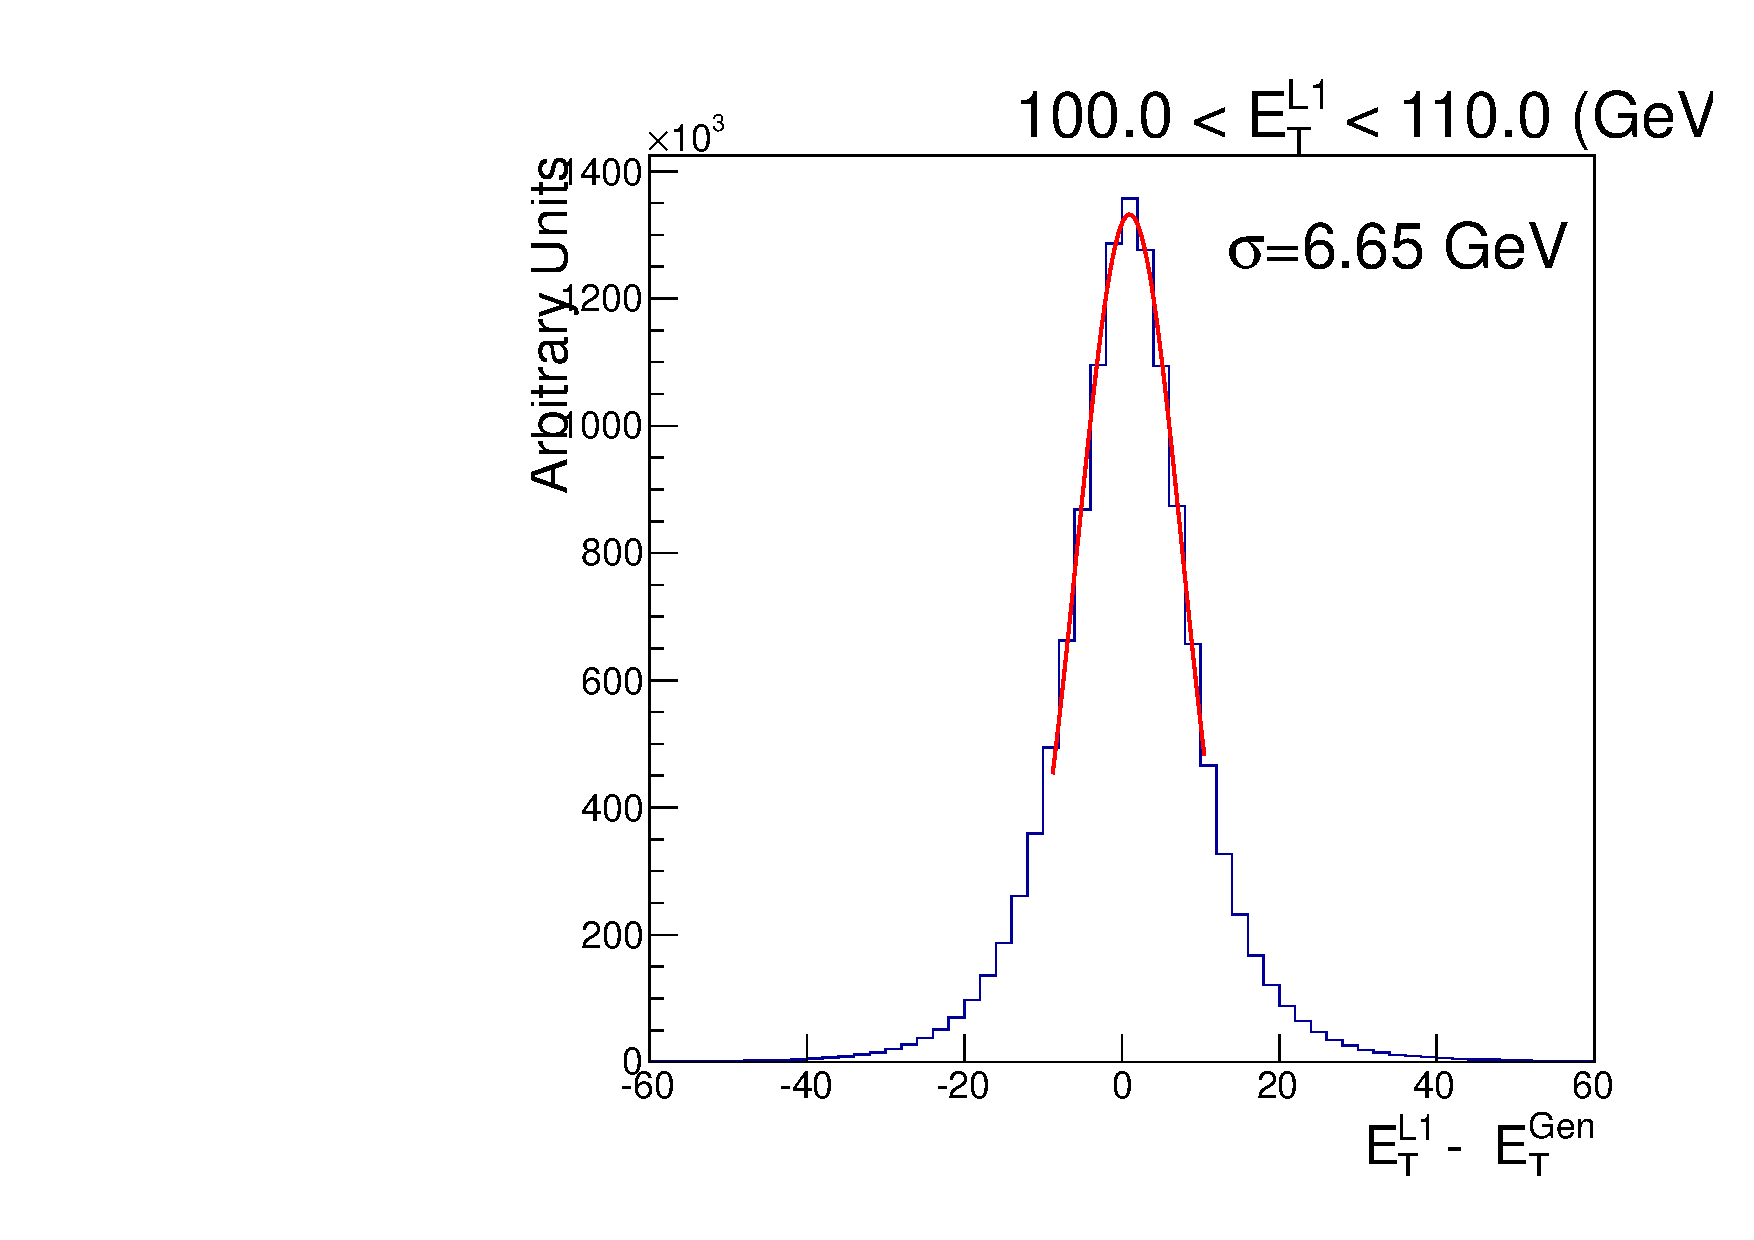
\includegraphics[width=0.32\textwidth]{detector/l1jet/gaussfits//ptBin_12_PtAll_pf.pdf}
    \caption{Part two of the distributions of $\Lonept-\Genpt$ in bins of $\Lonept$ of the corrected MC jets. 
	The fitted Gaussian is used to extract the resolution as a function of $\Lonept$.}
    \label{fig:mcresfits_pf_p2}
\end{figure}


